\chapter{PENGUJIAN DAN ANALISIS}
\label{chap:pengujiananalisis}

\section{Alat dan Bahan}
\label{sec:alatdanbahan}

\subsection{Perangkat Pelatihan Model \emph{Machine Learning}}

Pelatihan model dilakukan pada perangkat komputer dengan spesifikasi sebagai berikut:

\begin{table}[htbp]
  \centering
  \caption{Spesifikasi perangkat \emph{laptop} untuk pelatihan model}
  \label{tab:training_laptop_specs}
  \begin{tabular}{|l|l|}
  \hline
  \textbf{Prosesor} & Intel® Core™ i5-1235U \\
  \hline
  \textbf{GPU} & NVIDIA Geforce MX550 GDDR6 (2GB VRAM) \\
  \hline
  \textbf{RAM} & 16GB DDR4 \\
  \hline
  \textbf{Penyimpanan} & 512GB SSD M.2 PCIe \\
  \hline
  \textbf{Sistem Operasi} & Linux Ubuntu 22.04 Jammy Jellyfish \\
  \hline
  \textbf{Framework} & Tensorflow 2.15 \& PyTorch 2.3.0 \\
  \hline
  \textbf{Lingkungan Pengembangan} & Python 3.10.12 \\
  \hline
  \end{tabular}
\end{table}
Model yang digunakan adalah SSD MobileNetV2 yang dilatih menggunakan dataset kendaraan hasil anotasi sendiri dan milik dari penelitian Prismadika Yuniar \parencite*{prismadika2023}. Proses pelatihan dilakukan selama 30 dan 50 \emph{epoch} dengan batch size 16, learning rate 0.01, dan \emph{scheduler} antara CosineAnnealingLR dan MultiStepLR. Dataset terdiri dari masing-masing 165 dan 200 gambar kendaraan sebelum augmentasi, yang dibagi menjadi data latih (80\%) dan data validasi (20\%).

\subsection{\emph{Edge Device} untuk \emph{Inference}}

Untuk menjalankan sistem deteksi secara \emph{real-time}, model hasil pelatihan dikonversi dari format PyTorch Tensor (.pt) ke ONNX (.onnx) dengan tujuan untuk diimplementasikan pada perangkat edge. Pengujian dilakukan pada perangkat \emph{edge} yang memiliki spesifikasi sebagai berikut:

\subsubsection{Perangkat 1: NVIDIA Jetson Nano 4GB}

Perangkat pertama yang digunakan adalah NVIDIA Jetson Nano 4GB yang merupakan sistem berbasis ARM yang dirancang untuk aplikasi \emph{edge computing} dengan kemampuan grafis yang optimal. Jetson Nano memiliki GPU Maxwell dengan 128 CUDA \emph{cores} yang memungkinkan pemrosesan model \emph{deep learning} secara efisien. Kamera yang digunakan pada pengujian ini adalah Logitech C920 HD Pro USB \emph{Webcam} yang dapat memberikan kualitas video 1080p pada 30 FPS, cukup untuk pengolahan deteksi kendaraan secara \emph{real-time}. Tabel \ref{tab:jetson_nano_specs} menunjukkan spesifikasi perangkat Jetson Nano yang digunakan dalam penelitian ini.

\begin{table}[htbp]
  \centering
  \caption{Spesifikasi perangkat \emph{edge} pertama untuk \emph{inference}}
  \label{tab:jetson_nano_specs}
  \begin{tabular}{|l|l|}
  \hline
  \textbf{Perangkat} & NVIDIA Jetson Nano 4GB \\
  \hline
  \textbf{CPU} & Quad-core ARM Cortex-A57 MPCore processor \\
  \hline
  \textbf{GPU} & NVIDIA Maxwell 128 NVIDIA CUDA® \emph{cores} \\
  \hline
  \textbf{RAM} & 4 GB 64-bit LPDDR4, 1600MHz 25.6 GB/s \\
  \hline
  \textbf{Penyimpanan} & 16 GB eMMC 5.1 \\
  \hline
  \textbf{Sistem Operasi} & Linux Ubuntu 18.04 Bionic Beaver \\
  \hline
  \textbf{Kamera} & Logitech C920 HD Pro USB Webcam \\
  \hline
  \textbf{Lingkungan Pengembangan} & Python 3.6.9 \\
  \hline
  \end{tabular}
\end{table}

\subsubsection{Perangkat 2: Beelink Gemini T34}

Selain menggunakan Jetson Nano, perangkat kedua yang digunakan dalam pengujian adalah Beelink Gemini T34, sebuah mini PC dengan arsitektur x86 sebagai pembanding dengan Jetson Nano. Beelink Gemini T34 dilengkapi dengan prosesor Intel Celeron N3450 Quad-core untuk inferensi model \emph{deep learning}. Perangkat ini cocok untuk pengolahan data video, sehingga memudahkan implementasi model pada sistem gerbang tol. Tabel \ref{tab:beelink_t34_specs} menunjukkan spesifikasi perangkat Beelink Gemini T34 yang digunakan dalam penelitian ini.

\begin{table}[htbp]
  \centering
  \caption{Spesifikasi perangkat \emph{edge} kedua untuk \emph{inference}}
  \label{tab:beelink_t34_specs}
  \begin{tabular}{|l|l|}
  \hline
  \textbf{Perangkat} & Beelink Gemini T34 \\
  \hline
  \textbf{CPU} & Intel Celeron N3450 Quad-core \\
  \hline
  \textbf{GPU} & - \\
  \hline
  \textbf{RAM} & 8 GB DDR3L \\
  \hline
  \textbf{Penyimpanan} & 256 GB SSD M.2 SATA \\
  \hline
  \textbf{Sistem Operasi} & Linux Ubuntu 20.04 Focal Fossa \\
  \hline
  \textbf{Kamera} & Logitech C920 HD Pro USB Webcam \\
  \hline
  \textbf{Lingkungan Pengembangan} & Python 3.8.10 \\
  \hline
  \end{tabular}
\end{table}

Dengan penggunaan dua perangkat ini, yaitu NVIDIA Jetson Nano yang lebih fokus pada aplikasi \emph{edge} dengan akselerasi GPU untuk \emph{deep learning}, serta Beelink Gemini T34 yang menawarkan solusi berbasis prosesor Intel untuk komputasi ringan, pengujian dilakukan untuk melihat perbandingan performa dan kecocokan setiap perangkat untuk aplikasi deteksi kendaraan \emph{overdimensi}.

\subsection{Spesifikasi \emph{Server Cloud}}

Untuk mendukung pengolahan \emph{backend} dan pengelolaan data dari perangkat \emph{edge}, sistem ini menggunakan \emph{Virtual Private Server} (VPS) yang dihosting di \emph{cloud}. VPS ini digunakan untuk menjalankan layanan \emph{backend} seperti manajemen \emph{database}, penyimpanan data kendaraan yang terdeteksi, serta komunikasi antara perangkat \emph{edge} dan server \emph{cloud}. Tabel \ref{tab:cloud_server_specs} menunjukkan spesifikasi VPS yang digunakan dalam penelitian ini.

\begin{table}[htbp]
  \centering
  \caption{Spesifikasi \emph{Server Cloud} untuk Hosting \emph{Backend}}
  \label{tab:cloud_server_specs}
  \begin{tabular}{|l|l|}
  \hline
  \textbf{Provider} & Biznet Gio \\
  \hline
  \textbf{Tipe VPS} & Neo Lite \\
  \hline
  \textbf{CPU} & 1 vCPU (Intel Xeon) \\
  \hline
  \textbf{RAM} & 2 GB \\
  \hline
  \textbf{Penyimpanan} & 60 GB SSD \\
  \hline
  \textbf{Sistem Operasi} & Ubuntu 22.04 LTS \\
  \hline
  \textbf{IP Address} & Static Public IP \\
  \hline
  \textbf{Lingkungan Pengembangan} & Node.js v20.19.1  \\
  \hline
  \end{tabular}
\end{table}

\subsection{Lingkungan Pengujian}

Lingkungan pengujian alat dilakukan di Gerbang Tol Dupak 2, Genting Kalianak, Asem Rowo, Surabaya, Jawa Timur. Pengujian dilakukan pada hari Senin, 28 April 2025, Kamis 1 Mei 2025, dan Jumat 2 Mei 2025. Masing-masing hari pengujian dilakukan pada pukul 08:00 - 12:00 WIB. 

Perangkat kamera ditempatkan pada ketinggian 1 meter dari permukaan jalan dibantu dengan tripod dengan sudut kemiringan 45 derajat ke arah lajur kendaraan. Posisi ini dipilih untuk memastikan penangkapan gambar yang optimal dari bagian depan kendaraan yang melintasi gerbang tol. Jarak pengambilan gambar dari perangkat kamera ke objek kendaraan sekitar 2 meter. Gambar \ref{fig:testing_environment} menunjukkan setup perangkat pada lokasi pengujian.

% Tambahkan gambar setup pengujian
\begin{figure}[htbp]
  \centering
  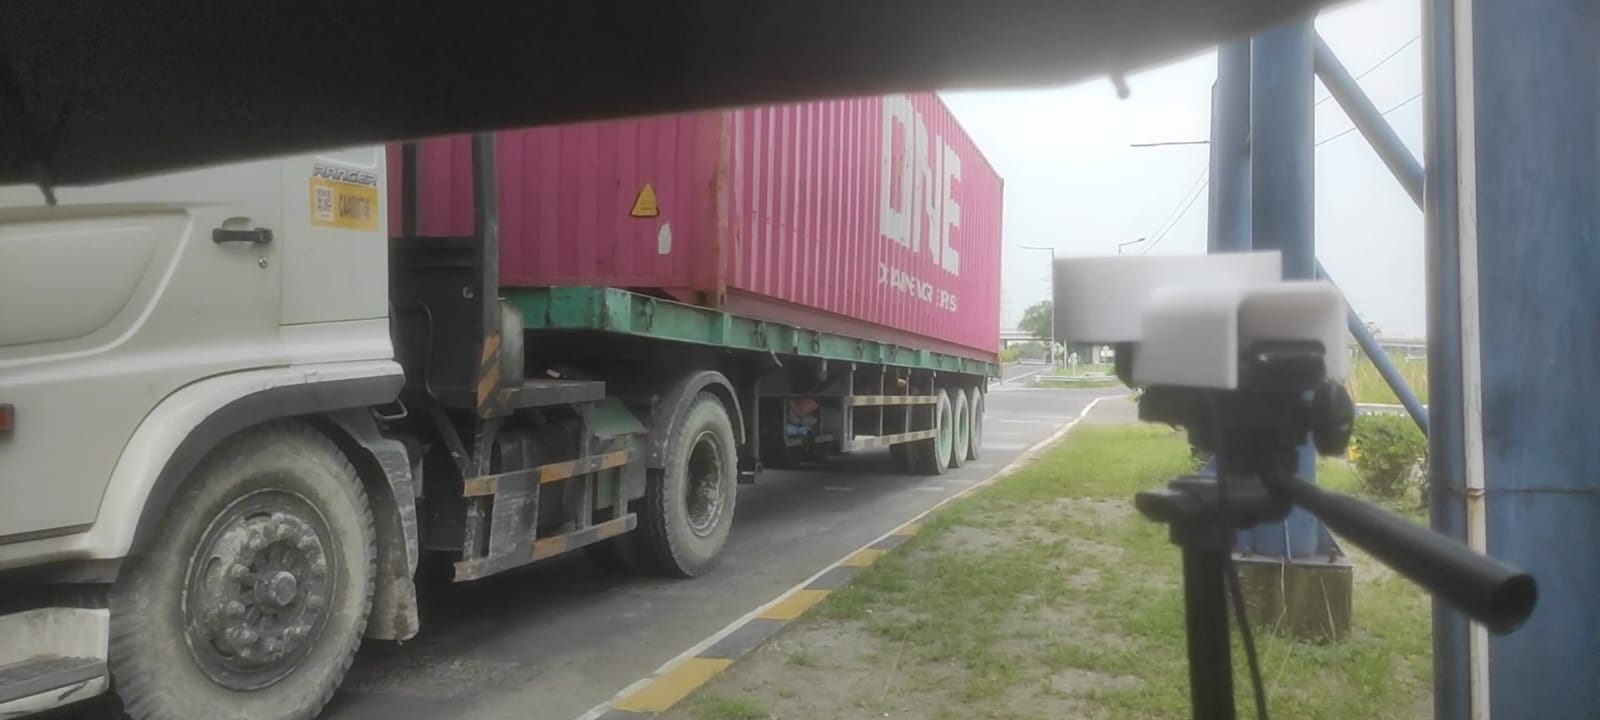
\includegraphics[width=0.84\textwidth]{gambar/bab4-test-dupak-kamera.jpeg}
  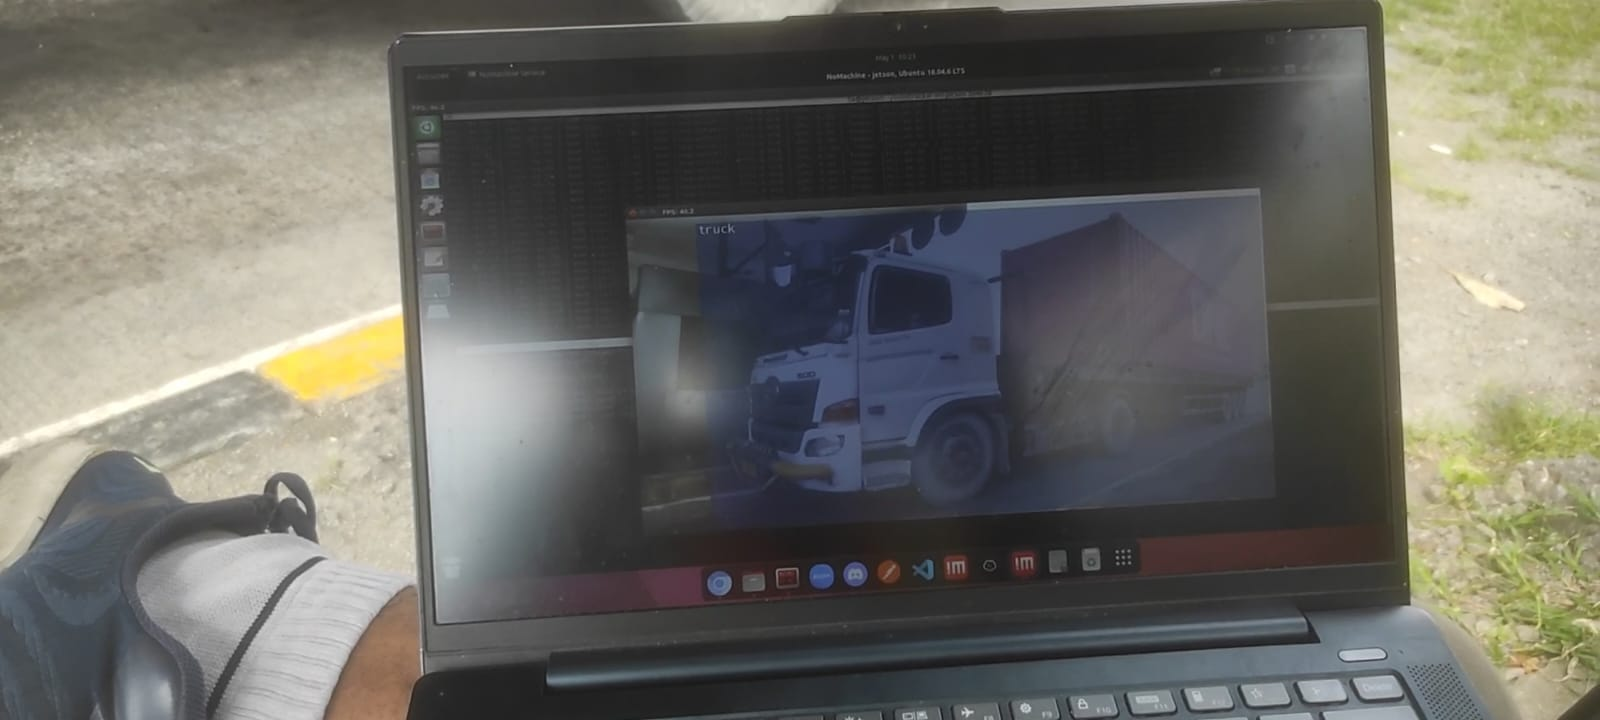
\includegraphics[width=0.84\textwidth]{gambar/bab4-test-dupak-monitor.jpeg}
  \caption{Setup perangkat pada lokasi pengujian di Gerbang Tol Dupak 2}
  \label{fig:testing_environment}
\end{figure}

Lalu lintas kendaraan selama pengujian tercatat rata-rata 120-150 kendaraan per jam dengan variasi jenis kendaraan meliputi mobil penumpang (55\%), truk ringan (25\%), truk sedang (15\%), dan kendaraan berat (5\%). Perangkat \emph{edge} ditempatkan di pinggir gerbang tol dengan koneksi internet berkecepatan 3-5 Mbps menggunakan \emph{hotspot} dari \emph{handphone} untuk transmisi data ke \emph{server cloud}. Pengaturan lingkungan pengujian ini dirancang untuk mensimulasikan kondisi nyata implementasi sistem di lapangan dengan mempertimbangkan berbagai faktor seperti posisi kamera, aliran lalu lintas, dan keterbatasan konektivitas yang mungkin dihadapi pada implementasi aktual. Hasil yang diperoleh dari pengujian dalam lingkungan ini diharapkan dapat memberikan gambaran yang akurat tentang performa sistem dalam kondisi operasional yang sebenarnya. 

\section{Model SSD-MobileNetV2}
\label{sec:model_ssd_mobilenetv2}

\subsection{Analisis Hasil Latih Model}

Hasil pelatihan model SSD-MobileNetV2 pada dataset kendaraan dianalisis berdasarkan beberapa metrik evaluasi yang umum digunakan dalam deteksi objek. Model dilatih dengan konfigurasi 16 batch size, learning rate 0.01, dan 4 konfigurasi berbeda, yaitu:

\begin{itemize}[nolistsep]
  \item 30 \emph{epoch} dan \emph{scheduler} CosineAnnealingLR
  \item 30 \emph{epoch} dan \emph{scheduler} MultiStepLR
  \item 50 \emph{epoch} dan \emph{scheduler} CosineAnnealingLR
  \item 50 \emph{epoch} dan \emph{scheduler} MultiStepLR
\end{itemize}\

Selama proses pelatihan, berbagai metrik dipantau untuk menganalisis konvergensi model, meliputi \emph{accuracy}, \emph{precision}, \emph{recall}, \emph{F1 score}, \emph{regression loss}, \emph{classification loss}, dan \emph{total loss}. Grafik di bawah ini menunjukkan hasil pelatihan untuk masing-masing konfigurasi.

\begin{figure}[htbp]
  \centering
  \begin{subfigure}{0.45\textwidth}
    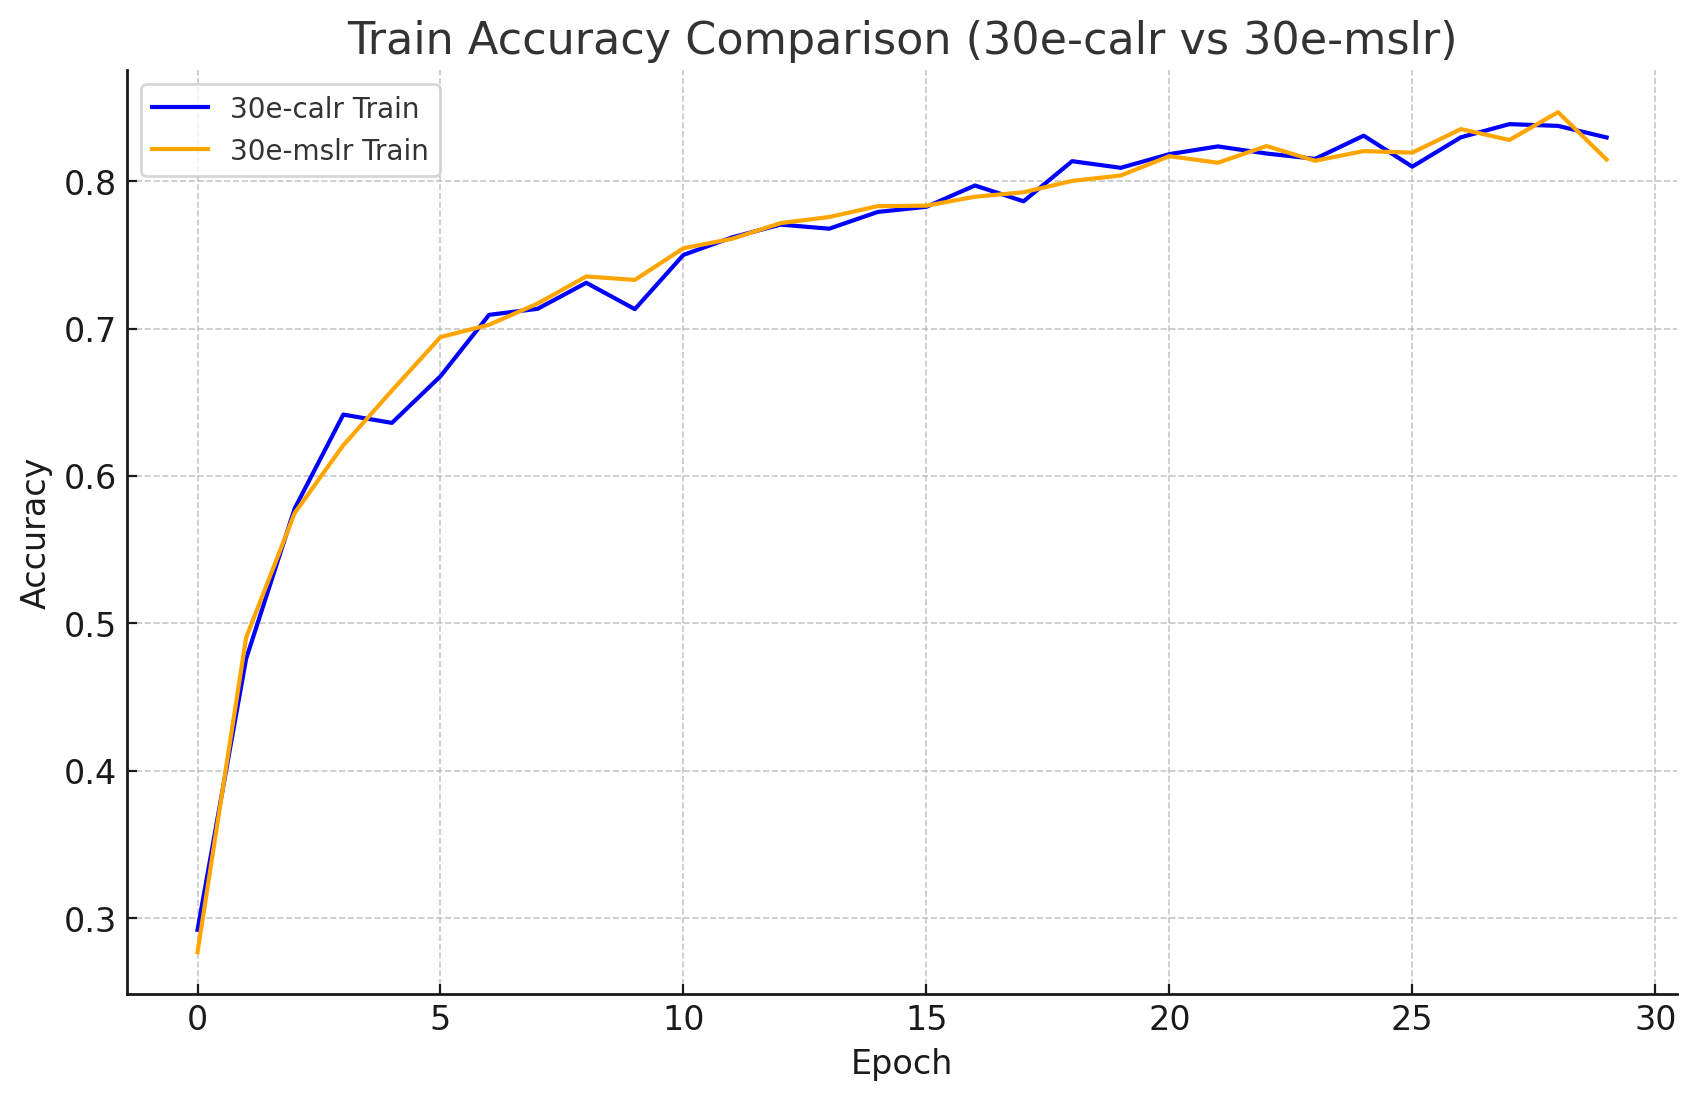
\includegraphics[width=\textwidth]{gambar/bab4-train-acc-30e.png}
    \caption{\emph{Accuracy} (\emph{training}) - 30 \emph{epoch}}
  \end{subfigure}
  \hfill
  \begin{subfigure}{0.45\textwidth}
    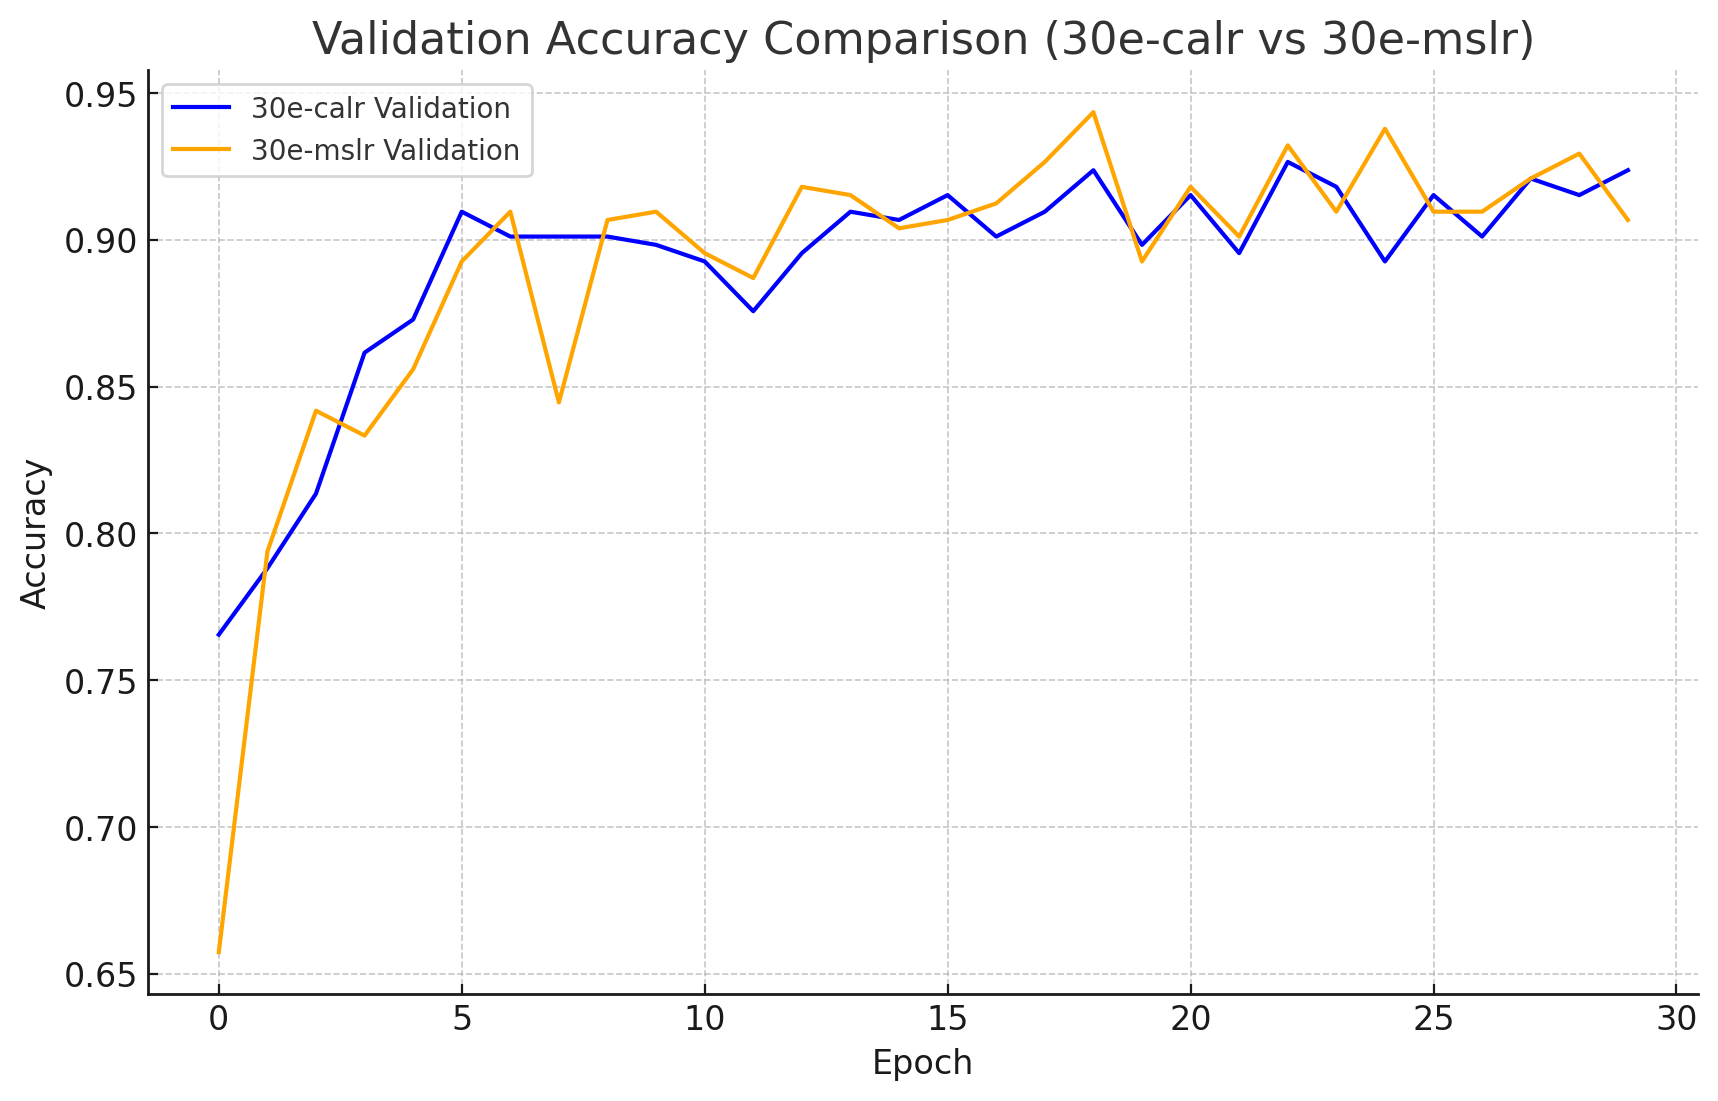
\includegraphics[width=\textwidth]{gambar/bab4-val-acc-30e.png}
    \caption{\emph{Accuracy} (\emph{validation}) - 30 \emph{epoch}}
  \end{subfigure}
  \begin{subfigure}{0.45\textwidth}
    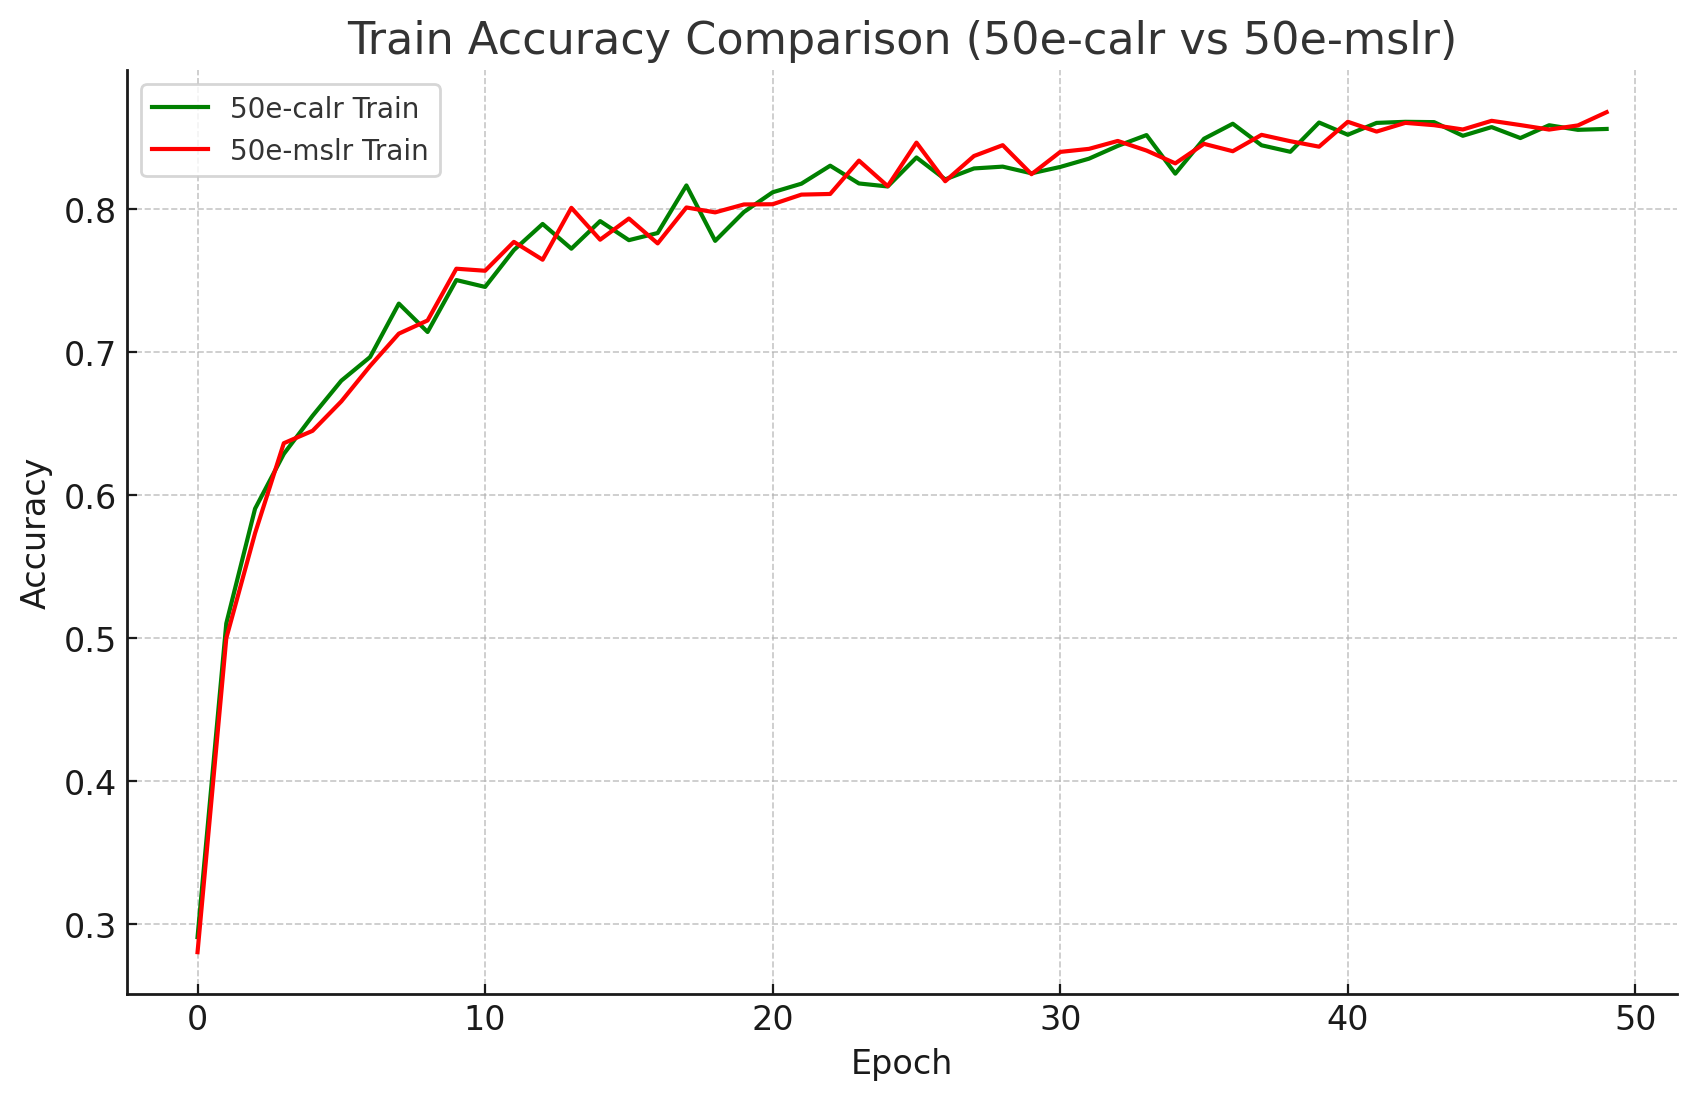
\includegraphics[width=\textwidth]{gambar/bab4-train-acc-50e.png}
    \caption{\emph{Accuracy} (\emph{training}) - 50 \emph{epoch}}
  \end{subfigure}
  \hfill
  \begin{subfigure}{0.45\textwidth}
    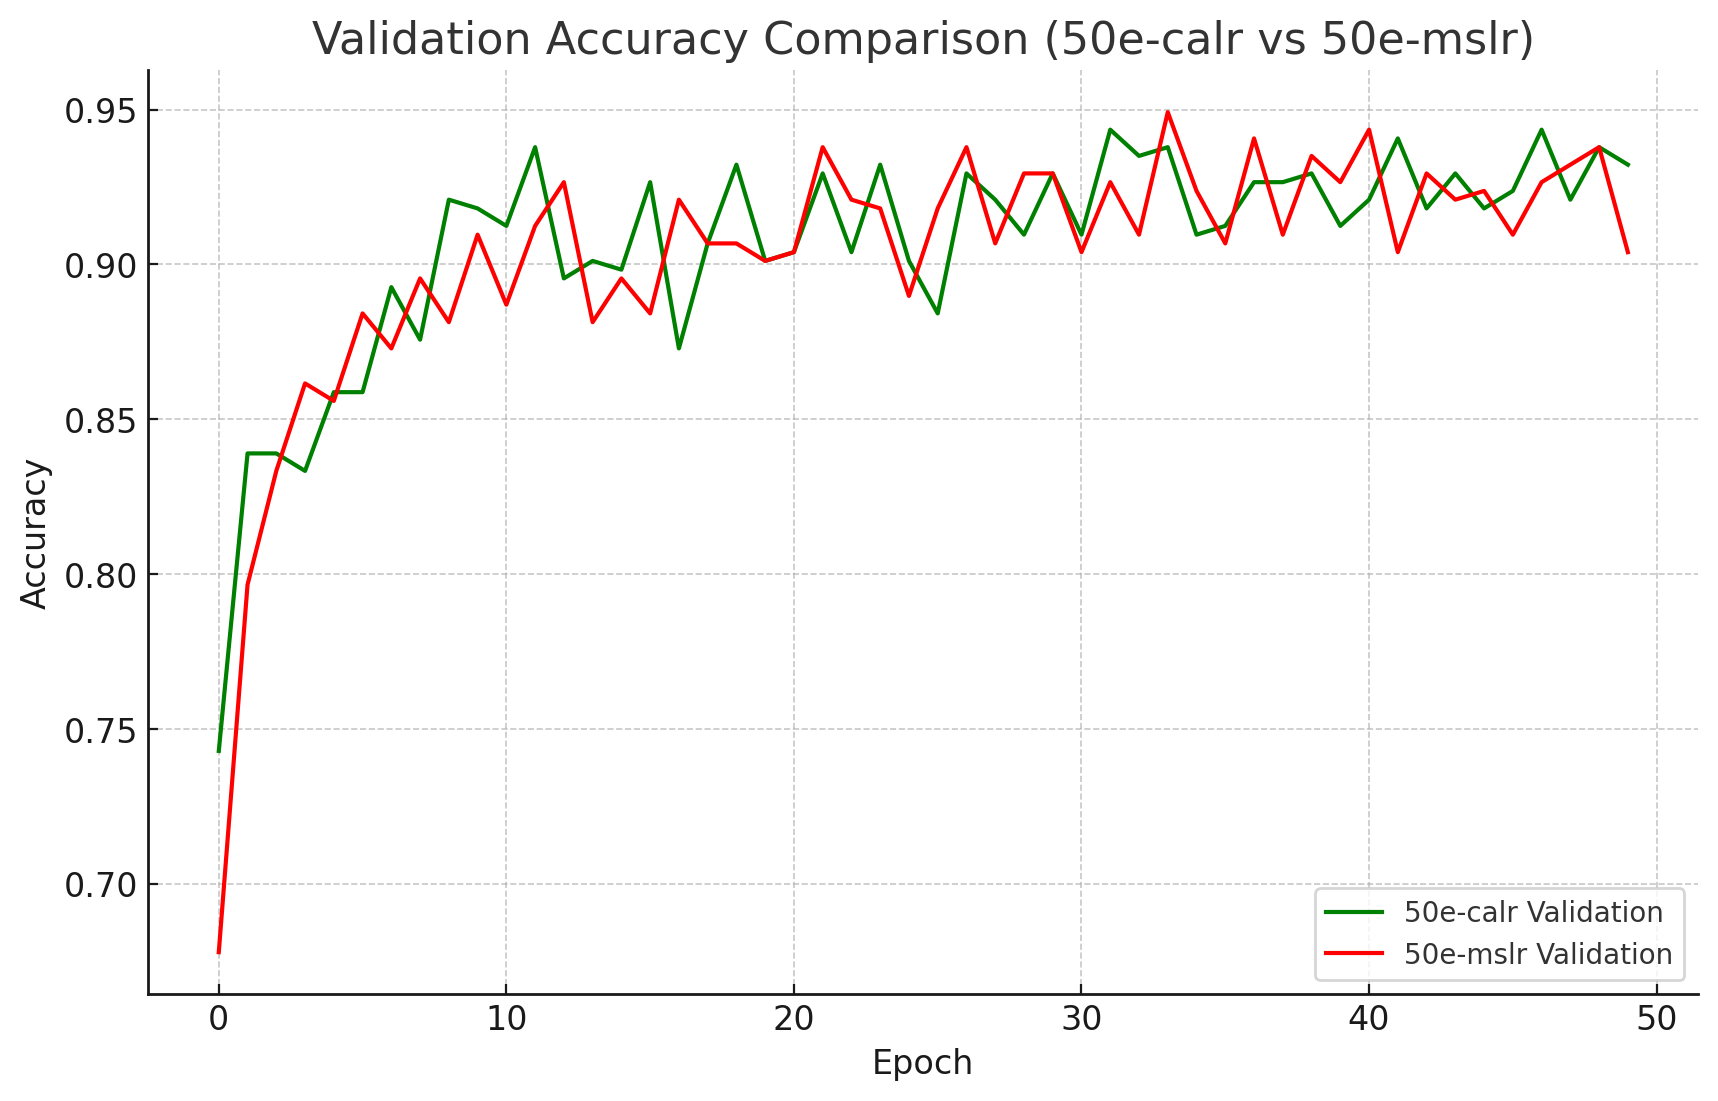
\includegraphics[width=\textwidth]{gambar/bab4-val-acc-50e.png}
    \caption{\emph{Accuracy} (\emph{validation}) - 50 \emph{epoch}}
  \end{subfigure}
  \caption{Kurva \emph{Accuracy} selama proses pelatihan model SSD-MobileNetV2}
  \label{fig:accuracy_curves}
\end{figure}

\begin{figure}[htbp]
  \centering
  \begin{subfigure}{0.45\textwidth}
    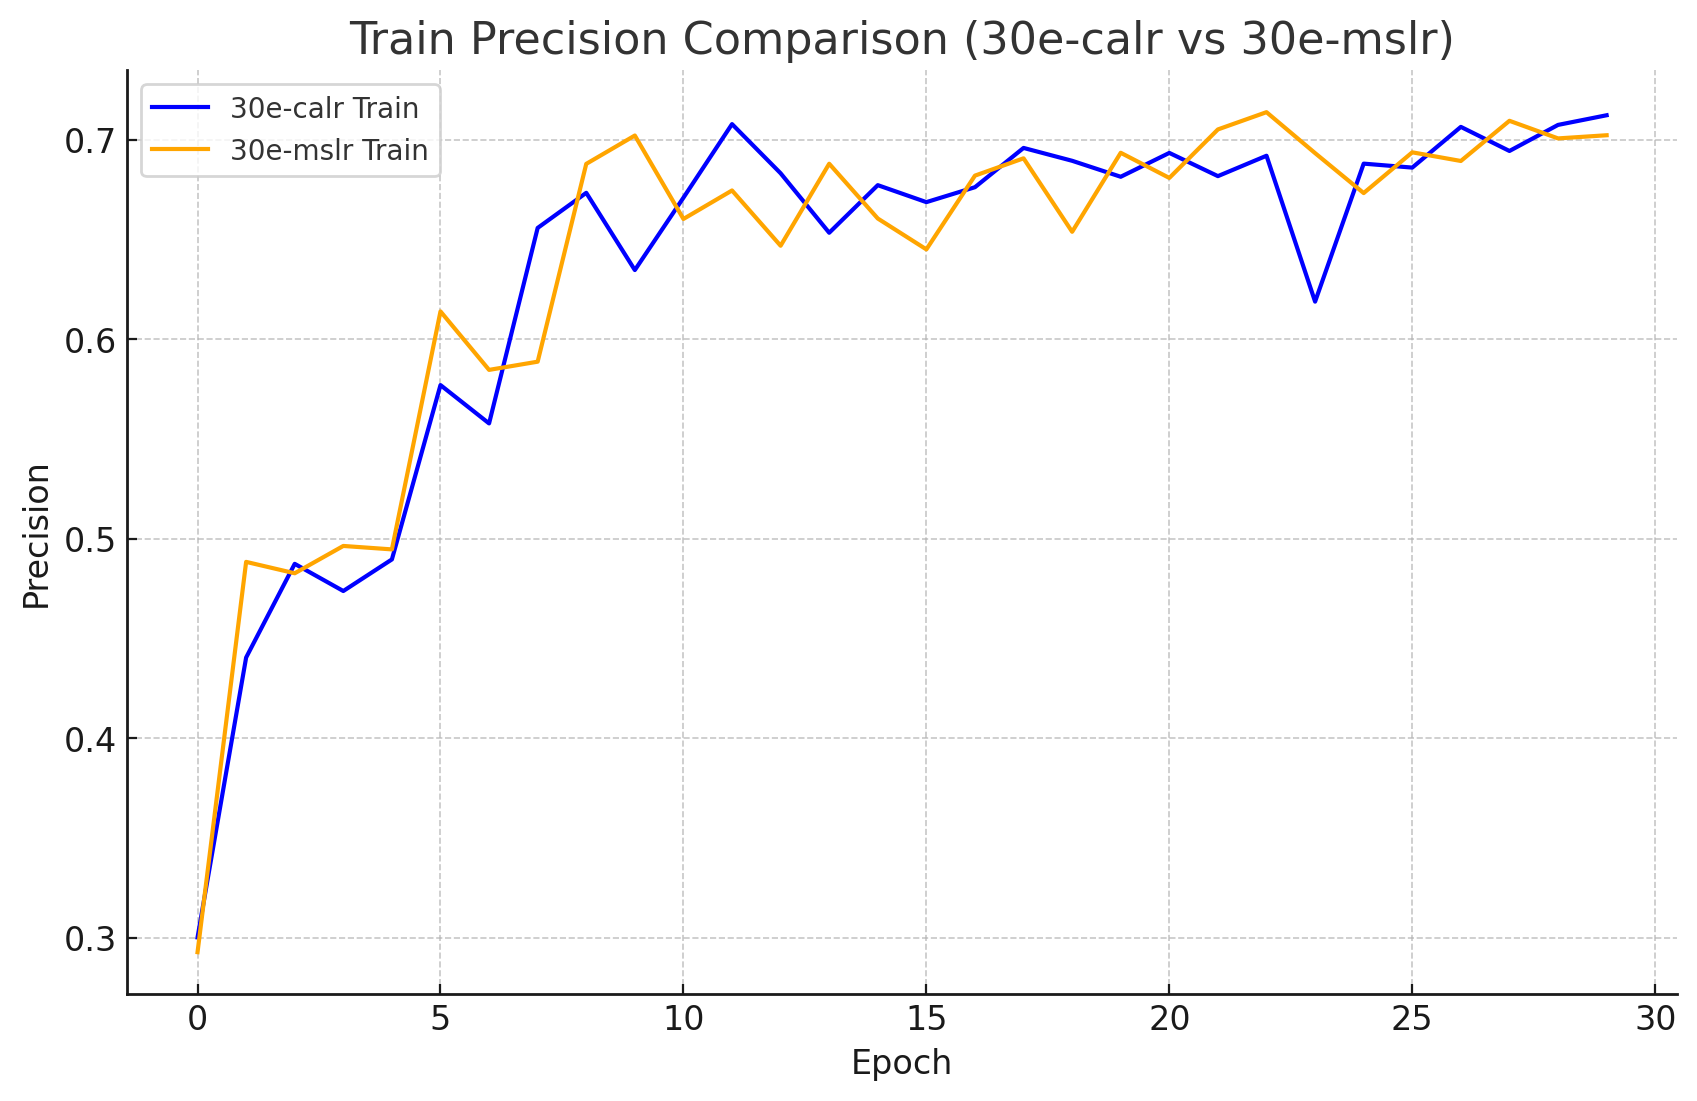
\includegraphics[width=\textwidth]{gambar/bab4-train-precision-30e.png}
    \caption{\emph{Precision} (\emph{training}) - 30 \emph{epoch}}
  \end{subfigure}
  \hfill
  \begin{subfigure}{0.45\textwidth}
    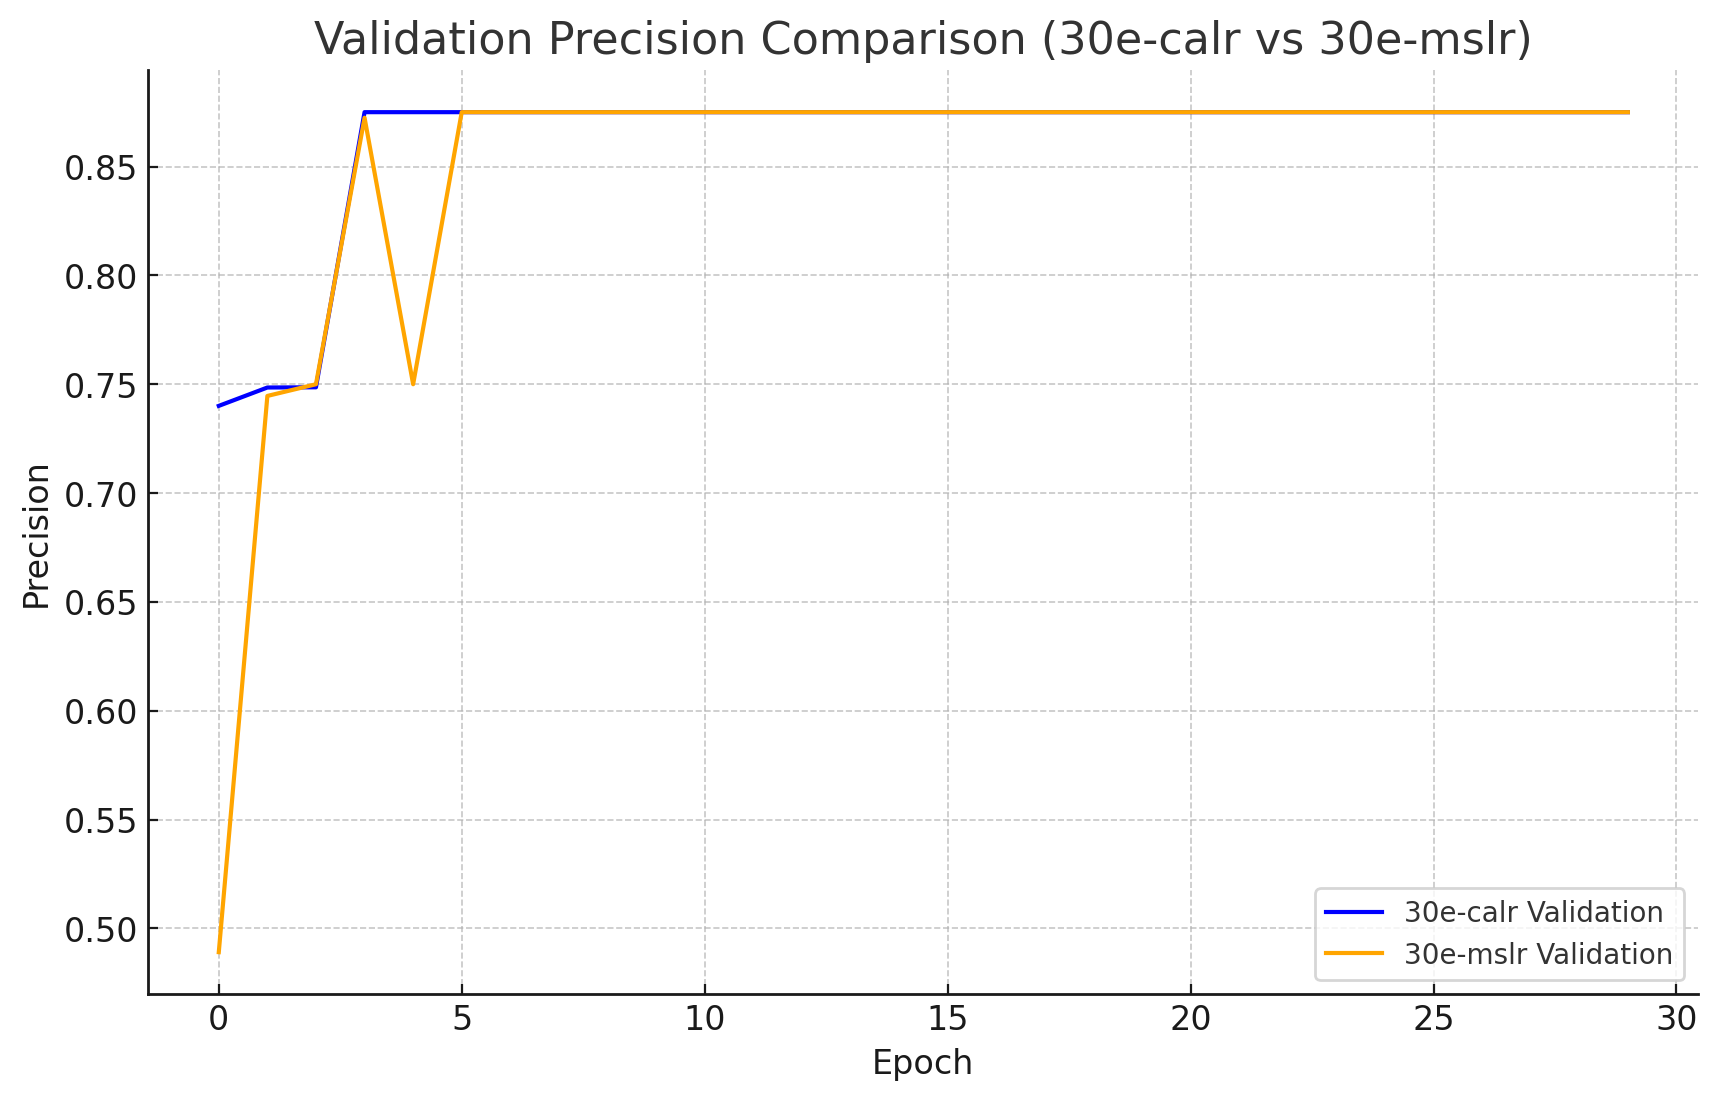
\includegraphics[width=\textwidth]{gambar/bab4-val-precision-30e.png}
    \caption{\emph{Precision} (\emph{validation}) - 30 \emph{epoch}}
  \end{subfigure}
  \hfill
  \begin{subfigure}{0.45\textwidth}
    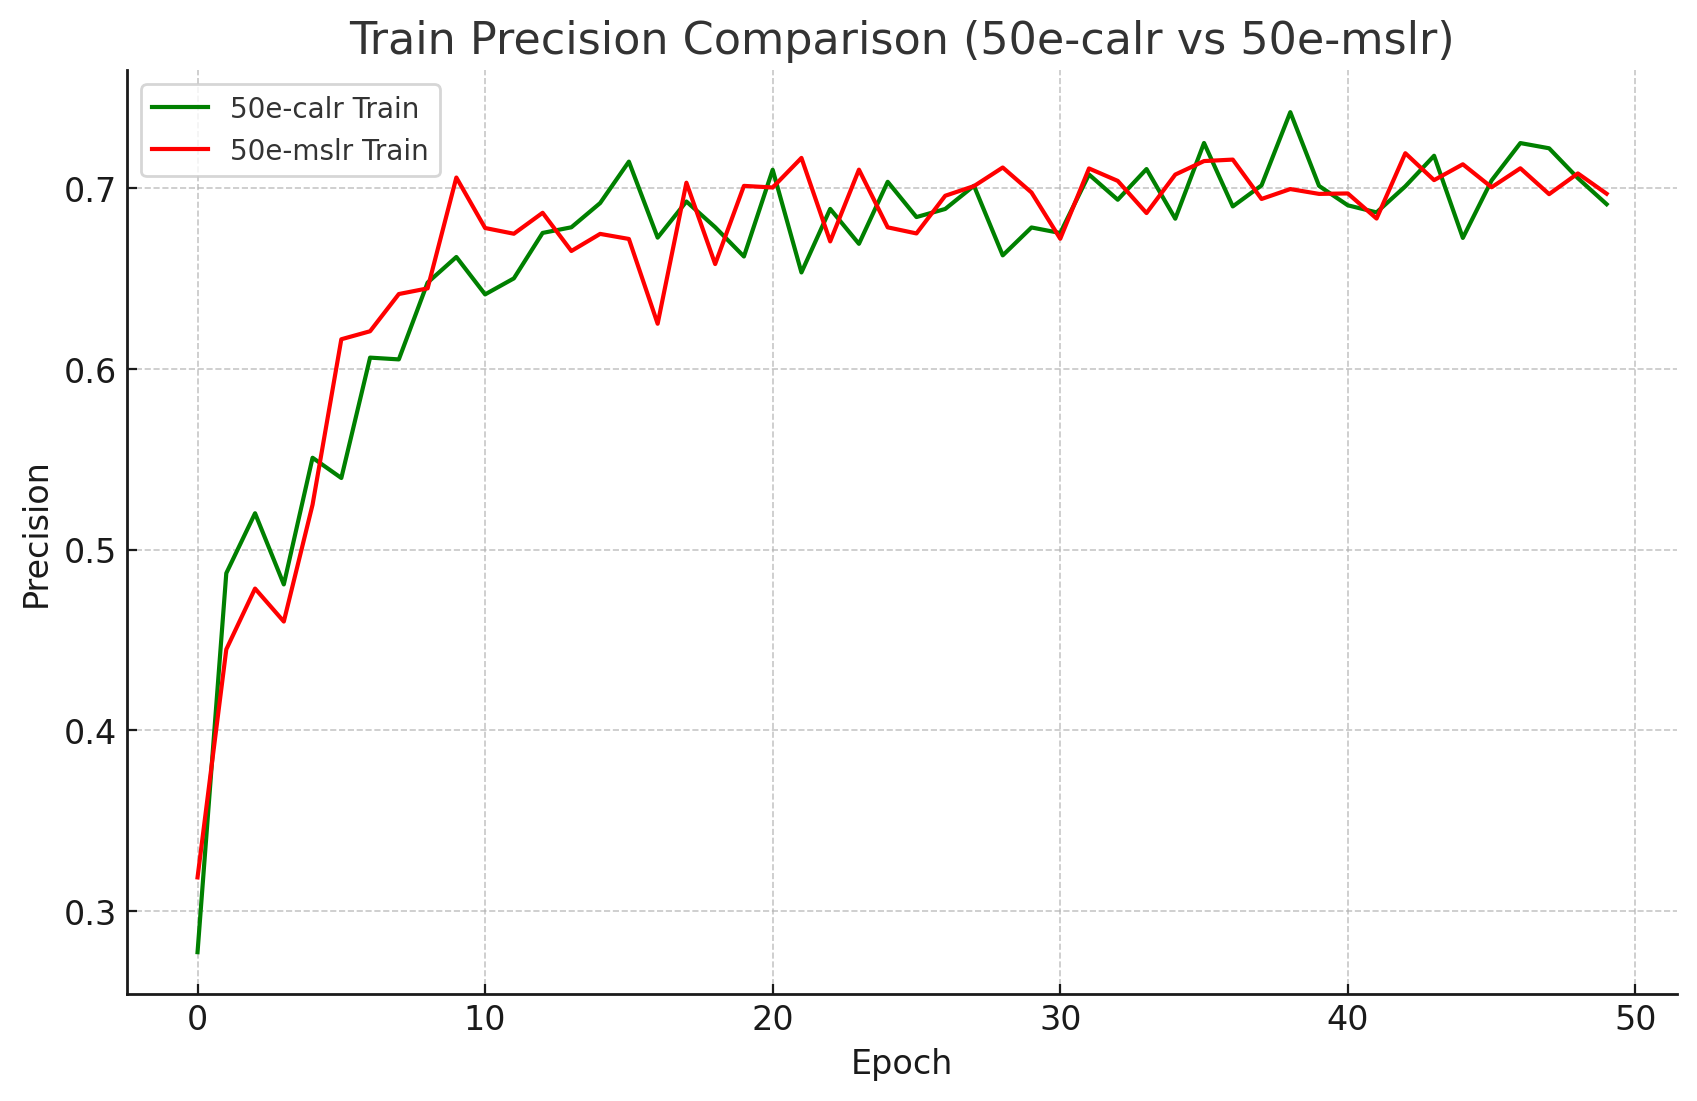
\includegraphics[width=\textwidth]{gambar/bab4-train-precision-50e.png}
    \caption{\emph{Precision} (\emph{training}) - 50 \emph{epoch}}
  \end{subfigure}
  \hfill
  \begin{subfigure}{0.45\textwidth}
    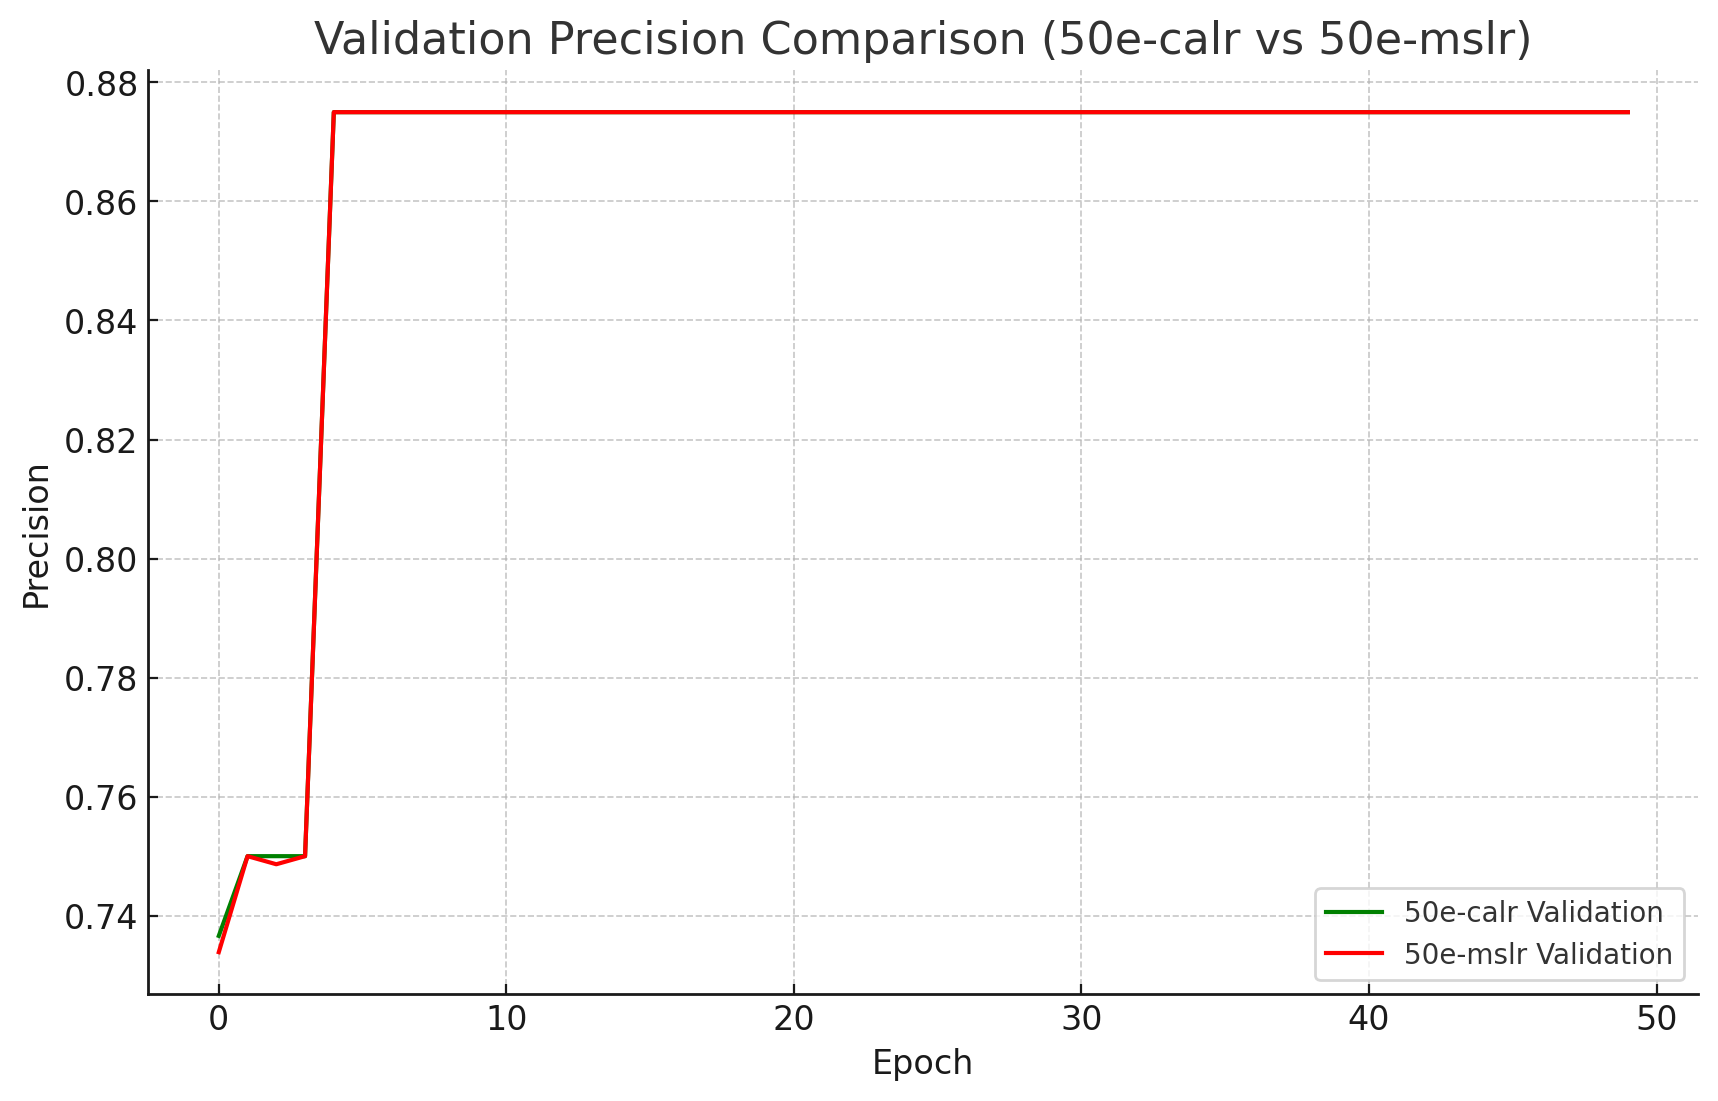
\includegraphics[width=\textwidth]{gambar/bab4-val-precision-50e.png}
    \caption{\emph{Precision} (\emph{validation}) - 50 \emph{epoch}}
  \end{subfigure}
  \caption{Kurva \emph{Precision} selama proses pelatihan model SSD-MobileNetV2}
  \label{fig:precision_curves}
\end{figure}

\begin{figure}[htbp]
  \centering
  \begin{subfigure}{0.45\textwidth}
    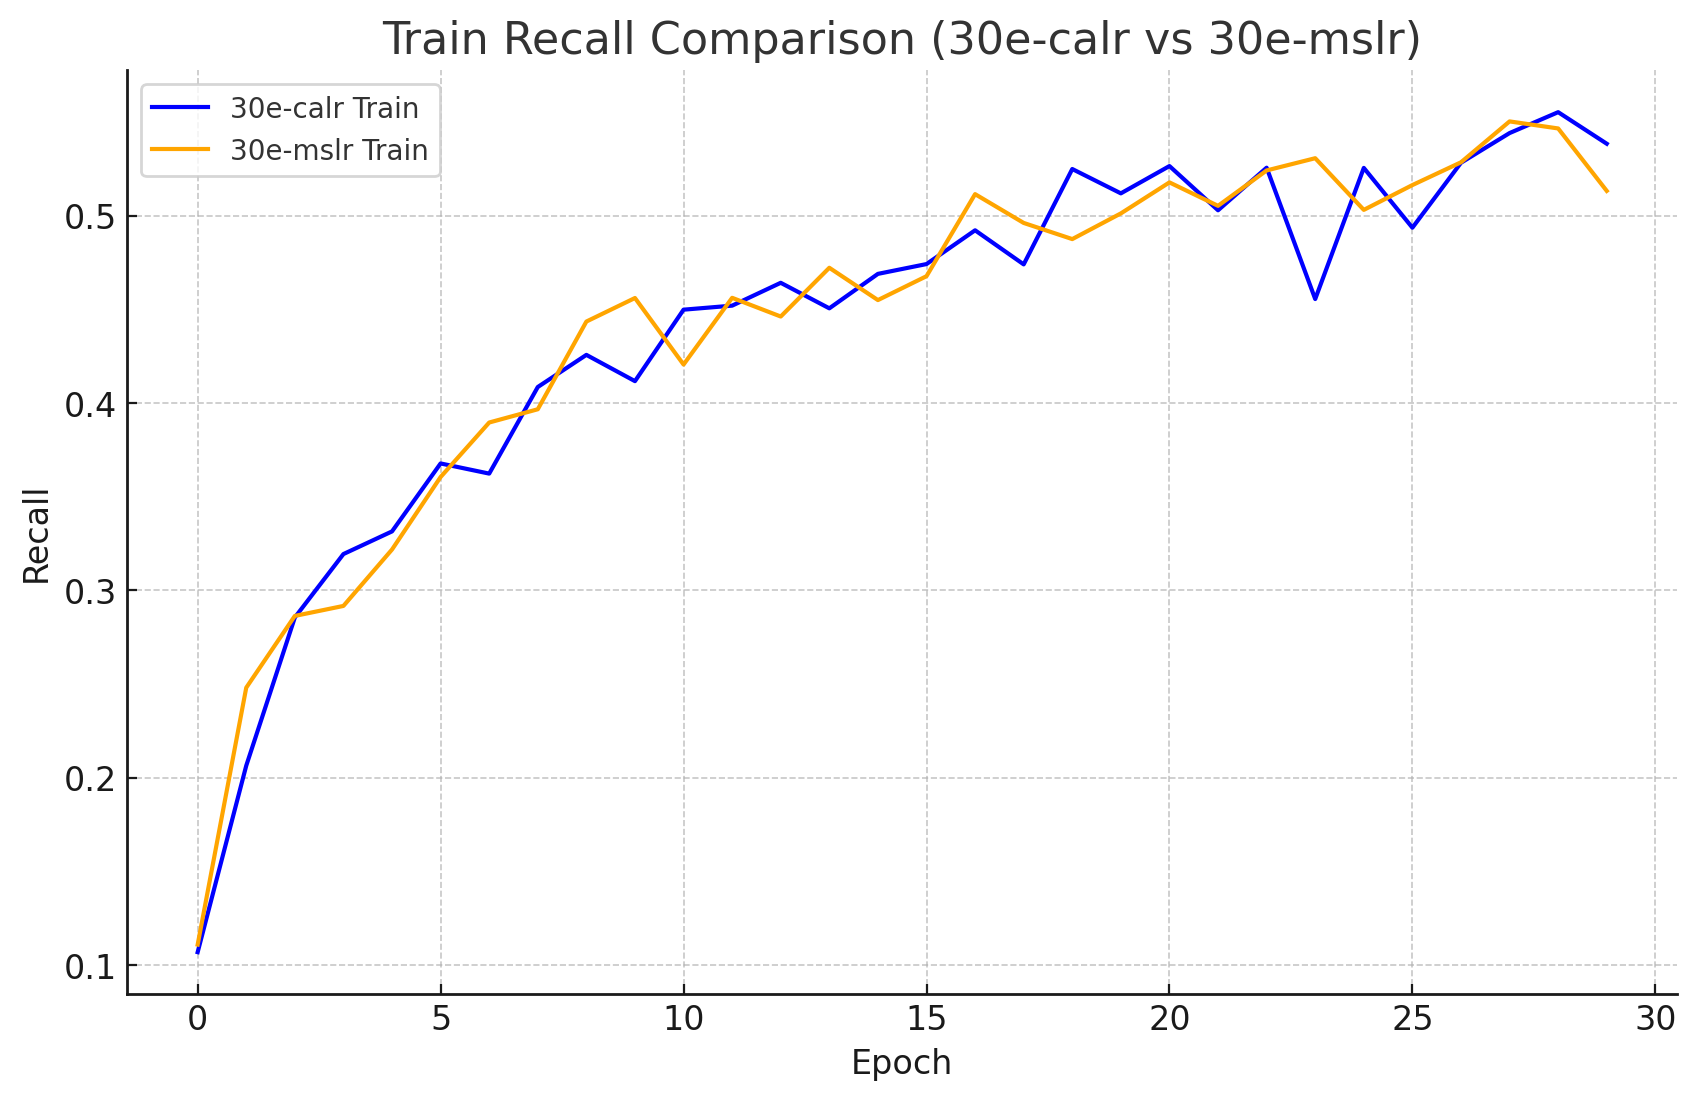
\includegraphics[width=\textwidth]{gambar/bab4-train-recall-30e.png}
    \caption{\emph{Recall} (\emph{training}) - 30 \emph{epoch}}
  \end{subfigure}
  \hfill
  \begin{subfigure}{0.45\textwidth}
    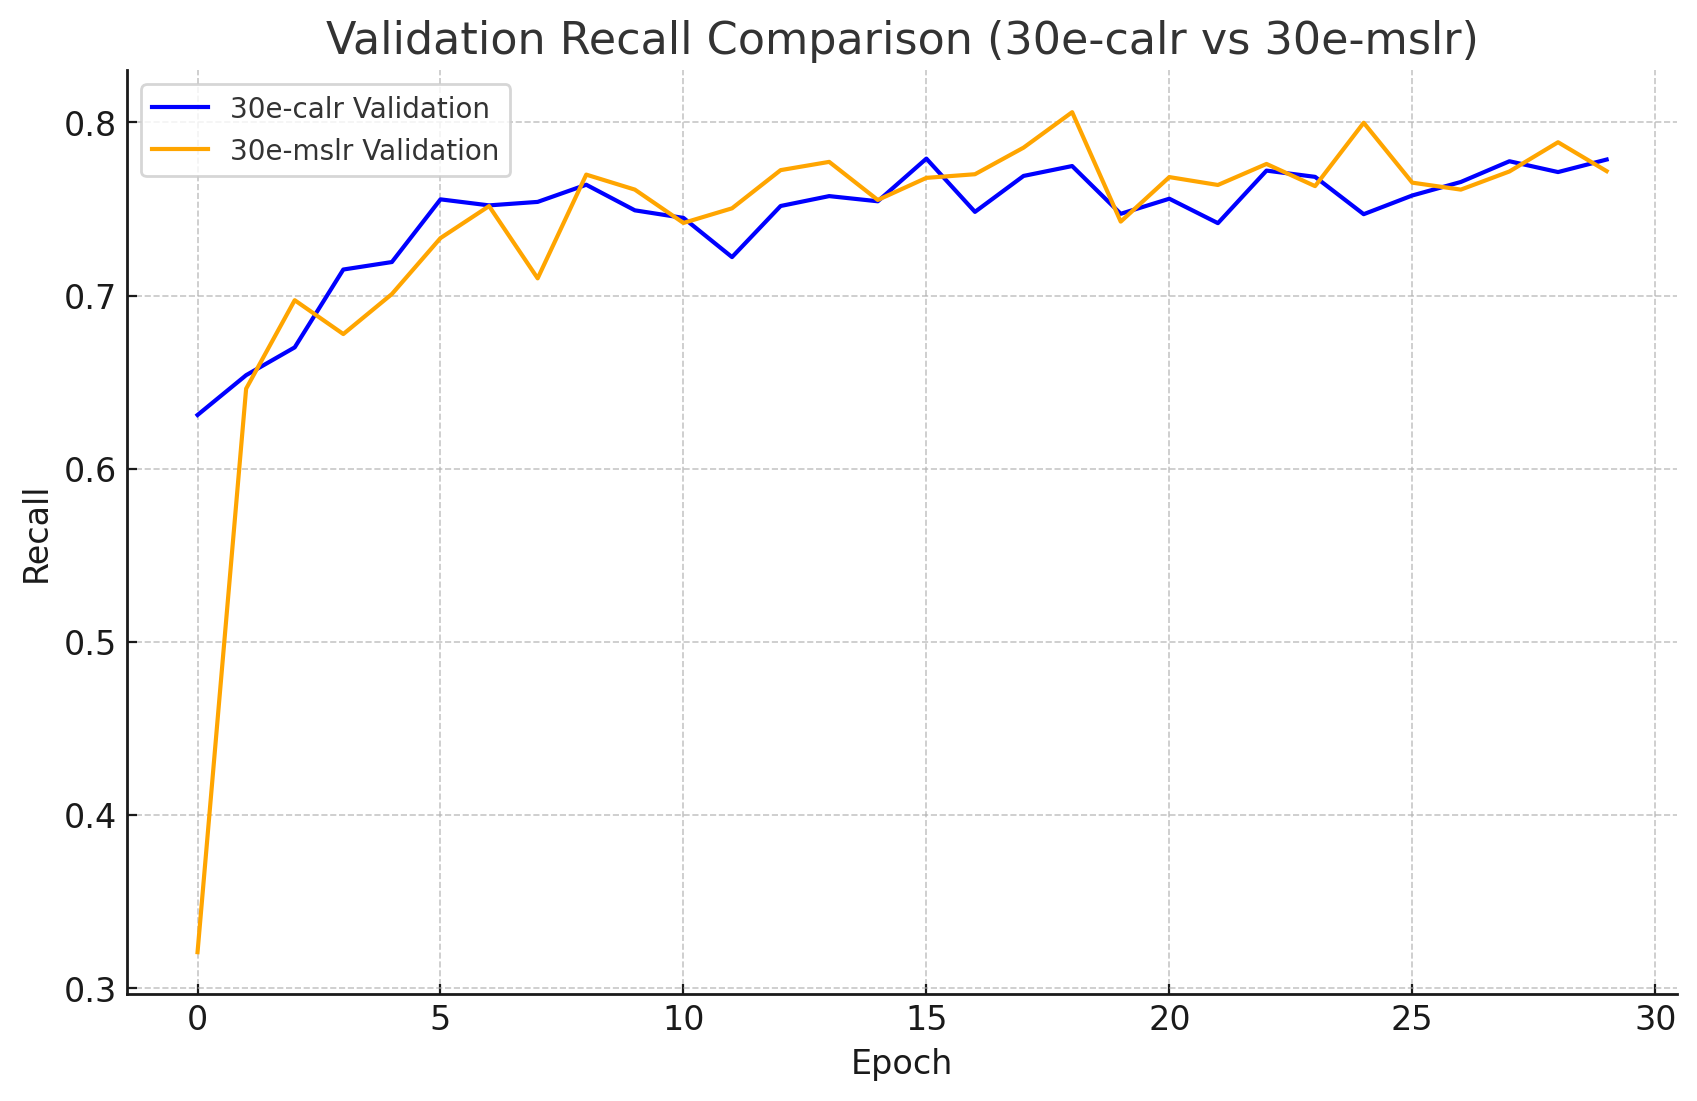
\includegraphics[width=\textwidth]{gambar/bab4-val-recall-30e.png}
    \caption{\emph{Recall} (\emph{validation}) - 30 \emph{epoch}}
  \end{subfigure}
  \hfill
  \begin{subfigure}{0.45\textwidth}
    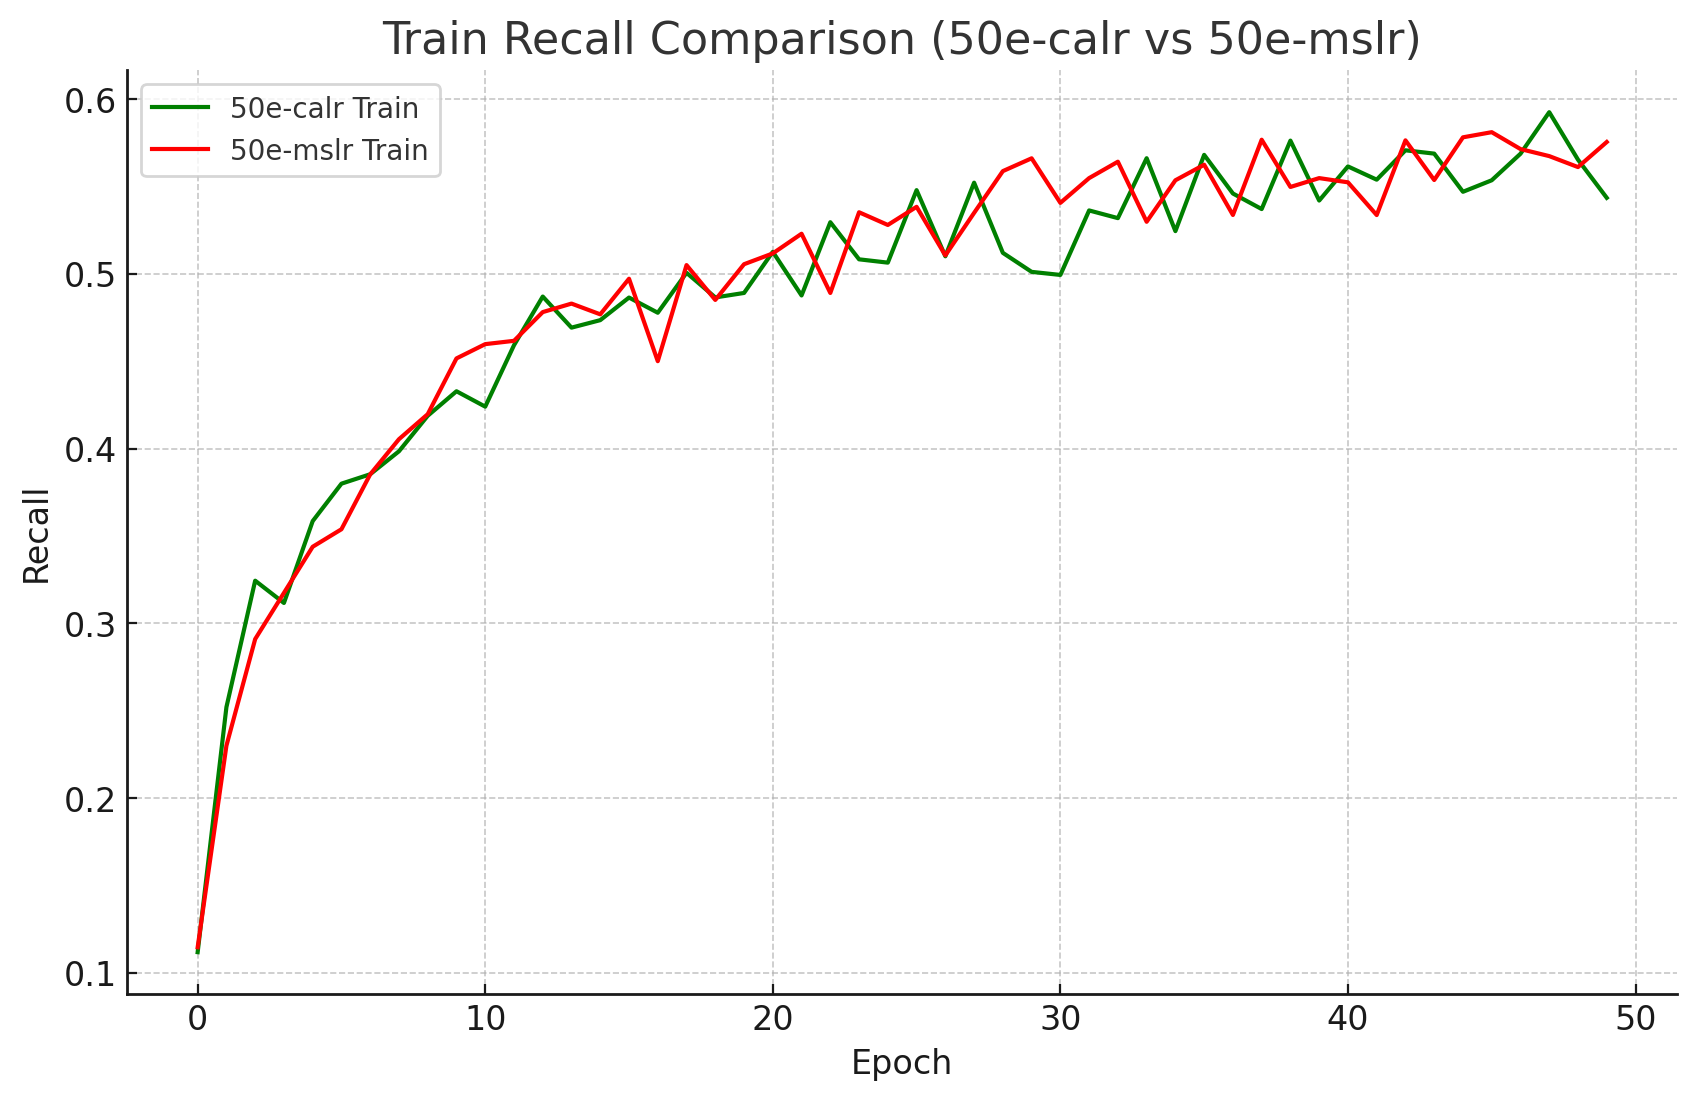
\includegraphics[width=\textwidth]{gambar/bab4-train-recall-50e.png}
    \caption{\emph{Recall} (\emph{training}) - 50 \emph{epoch}}
  \end{subfigure}
  \hfill
  \begin{subfigure}{0.45\textwidth}
    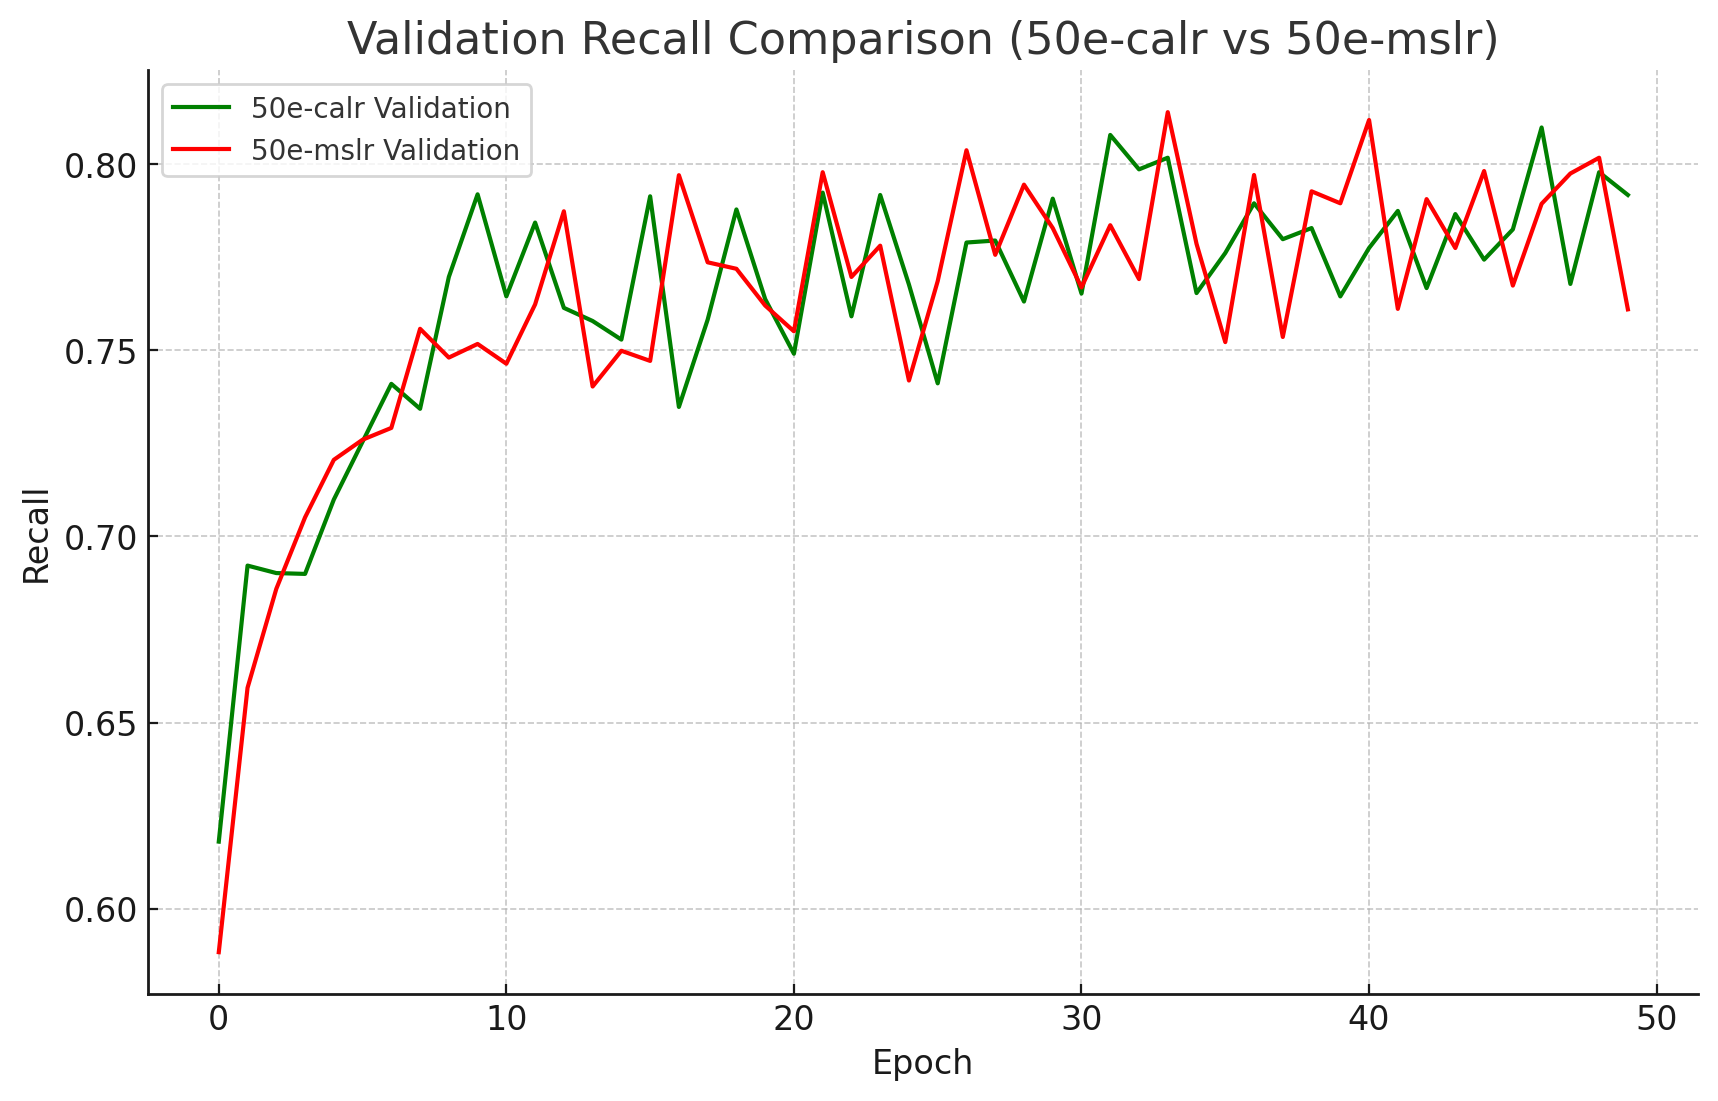
\includegraphics[width=\textwidth]{gambar/bab4-val-recall-50e.png}
    \caption{\emph{Recall} (\emph{validation}) - 50 \emph{epoch}}
  \end{subfigure}
  \caption{Kurva \emph{Recall} selama proses pelatihan model SSD-MobileNetV2}
  \label{fig:recall_curves}
\end{figure}

\begin{figure}[htbp]
  \centering
  \begin{subfigure}{0.45\textwidth}
    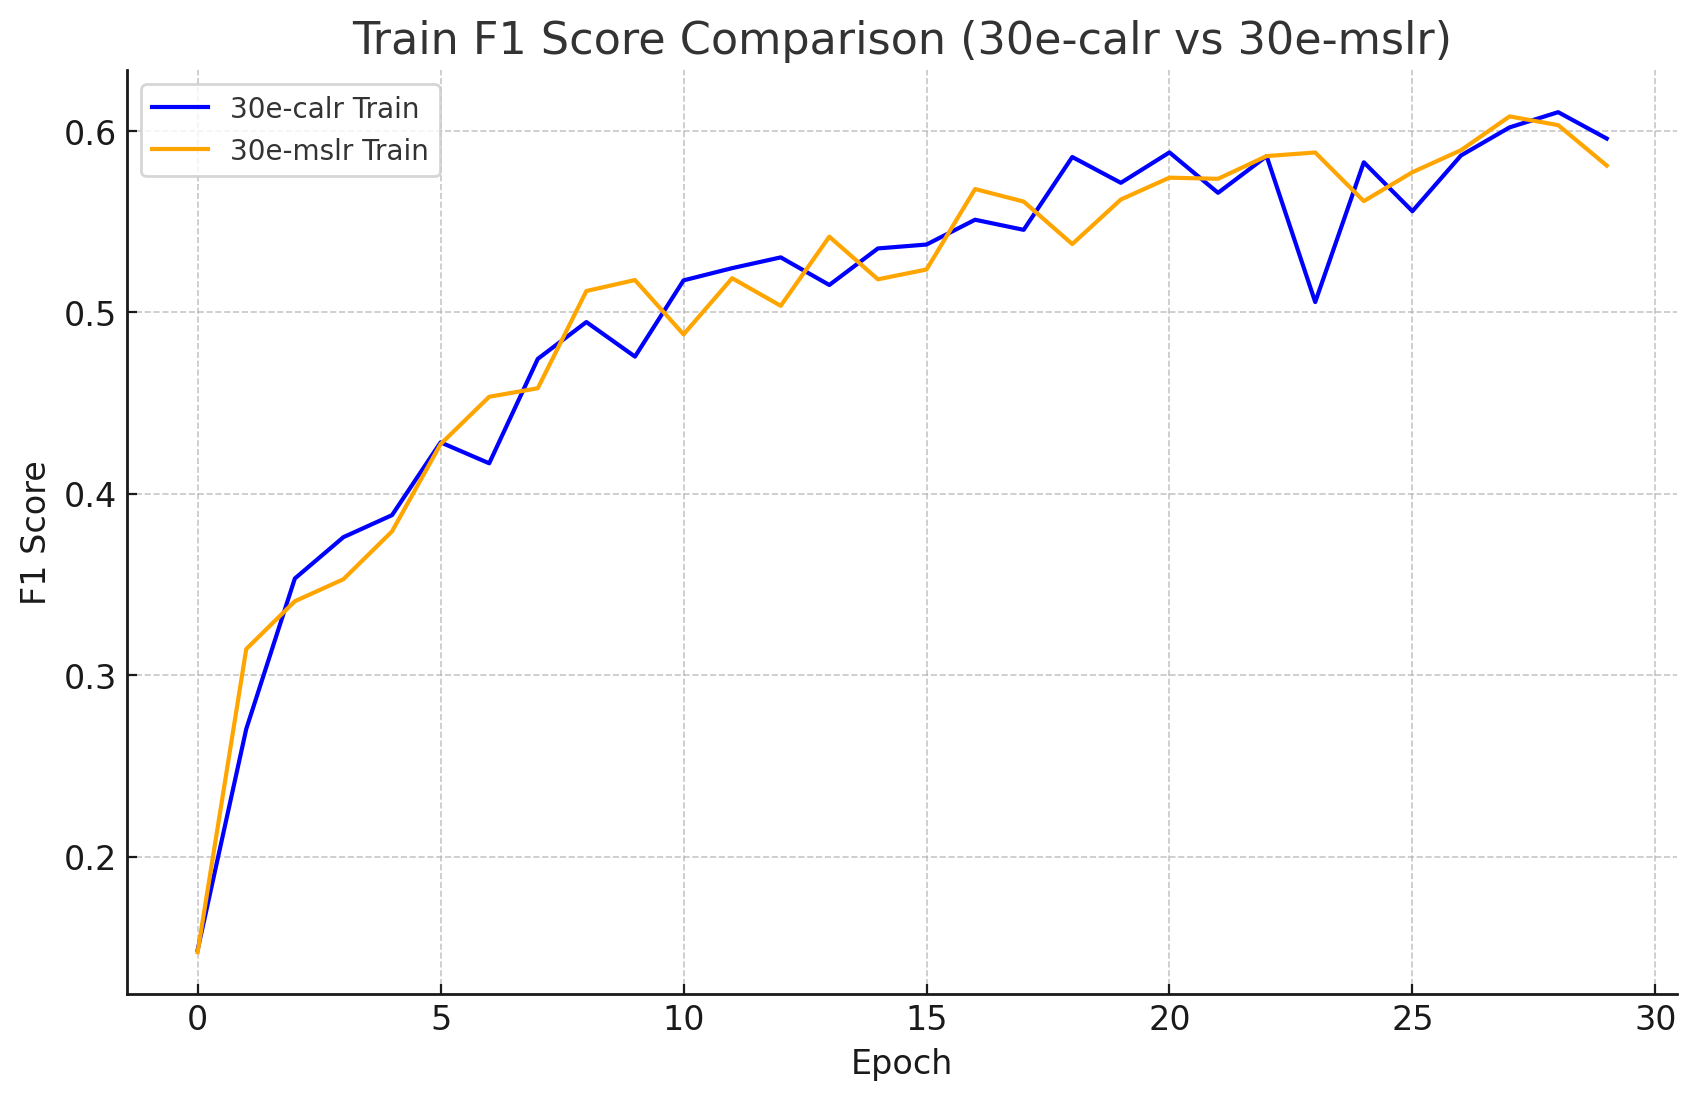
\includegraphics[width=\textwidth]{gambar/bab4-train-f1-score-30e.png}
    \caption{\emph{F1 Score} (\emph{training}) - 30 \emph{epoch}}
  \end{subfigure}
  \hfill
  \begin{subfigure}{0.45\textwidth}
    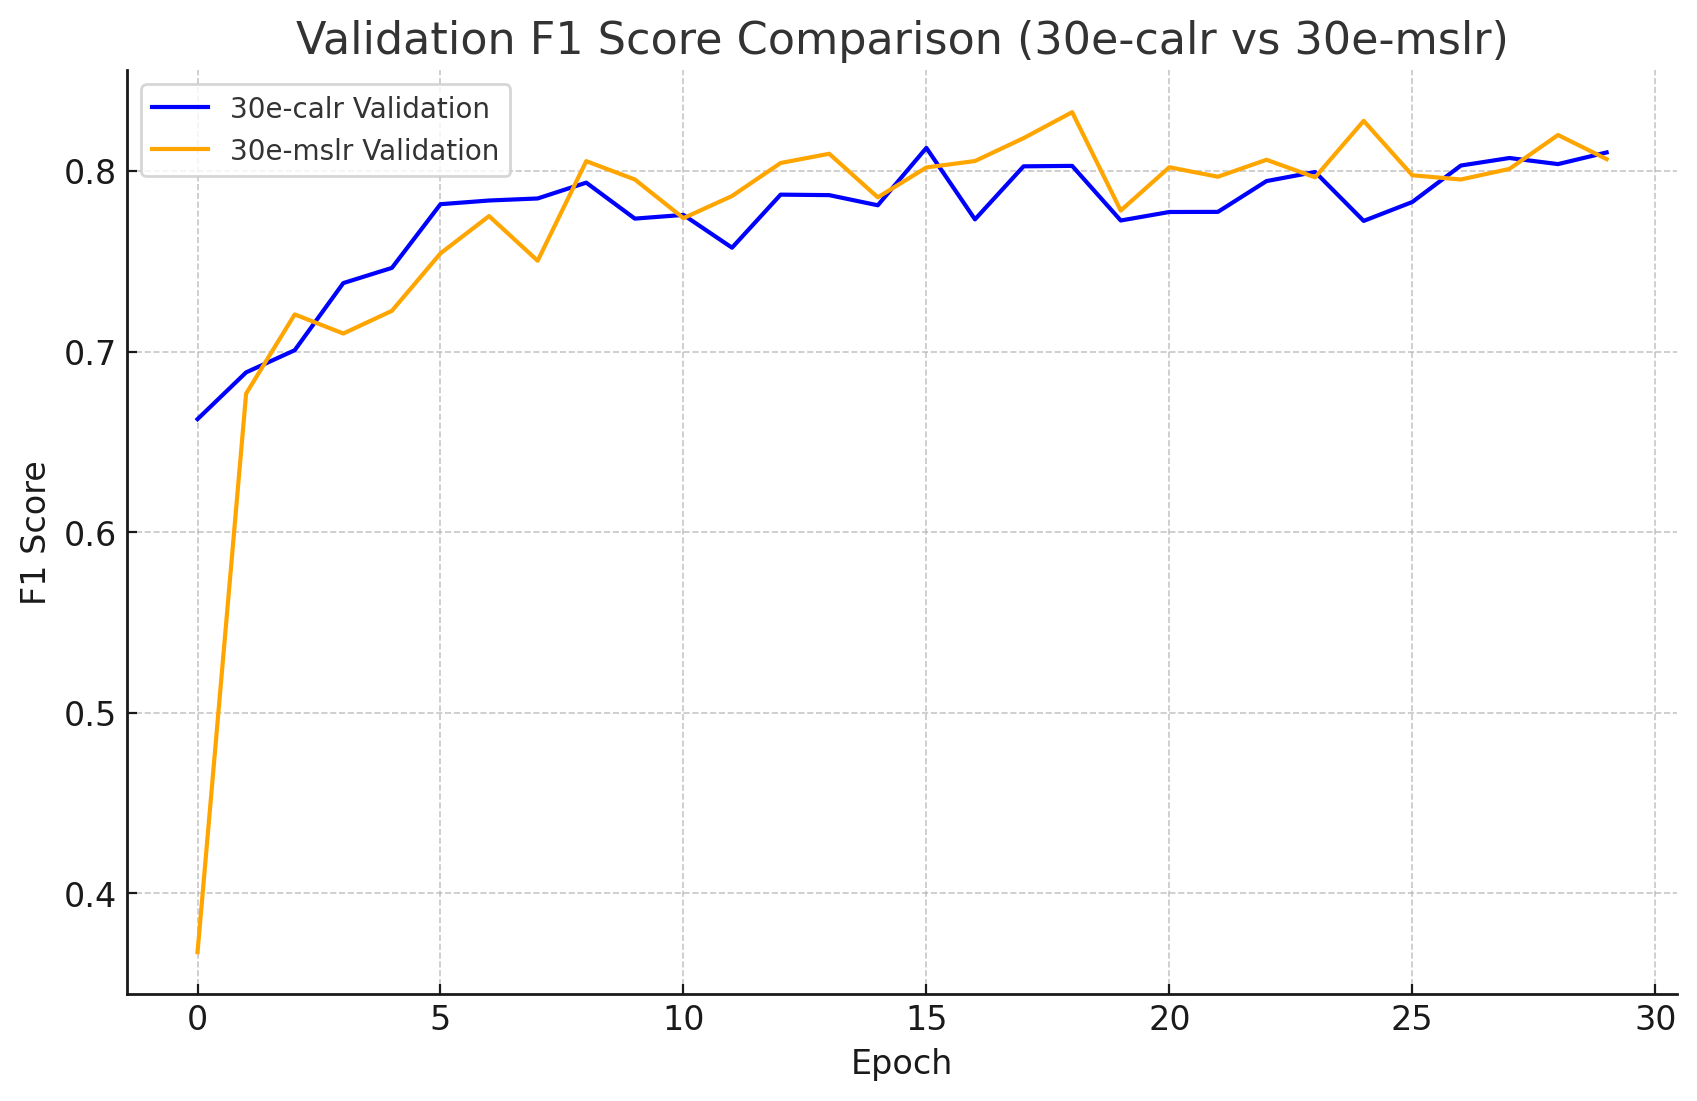
\includegraphics[width=\textwidth]{gambar/bab4-val-f1-score-30e.png}
    \caption{\emph{F1 Score} (\emph{validation}) - 30 \emph{epoch}}
  \end{subfigure}
  \hfill
  \begin{subfigure}{0.45\textwidth}
    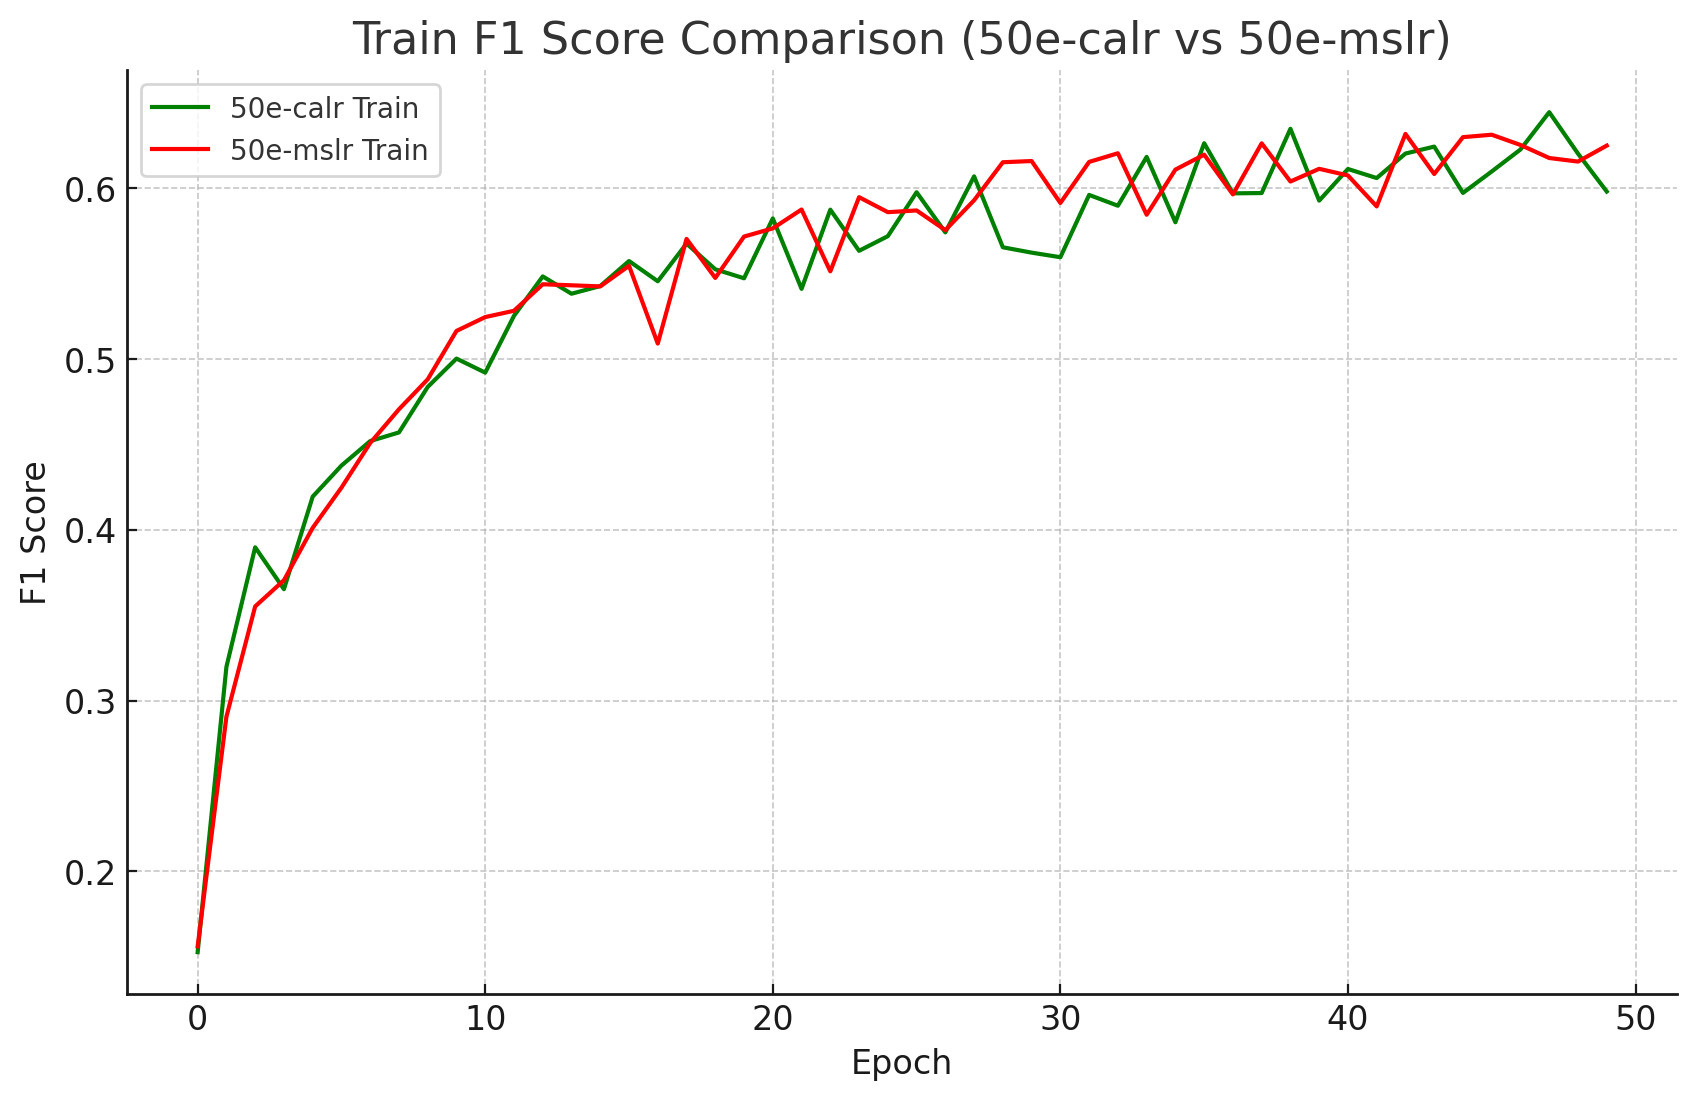
\includegraphics[width=\textwidth]{gambar/bab4-train-f1-score-50e.png}
    \caption{\emph{F1 Score} (\emph{training}) - 50 \emph{epoch}}
  \end{subfigure}
  \hfill
  \begin{subfigure}{0.45\textwidth}
    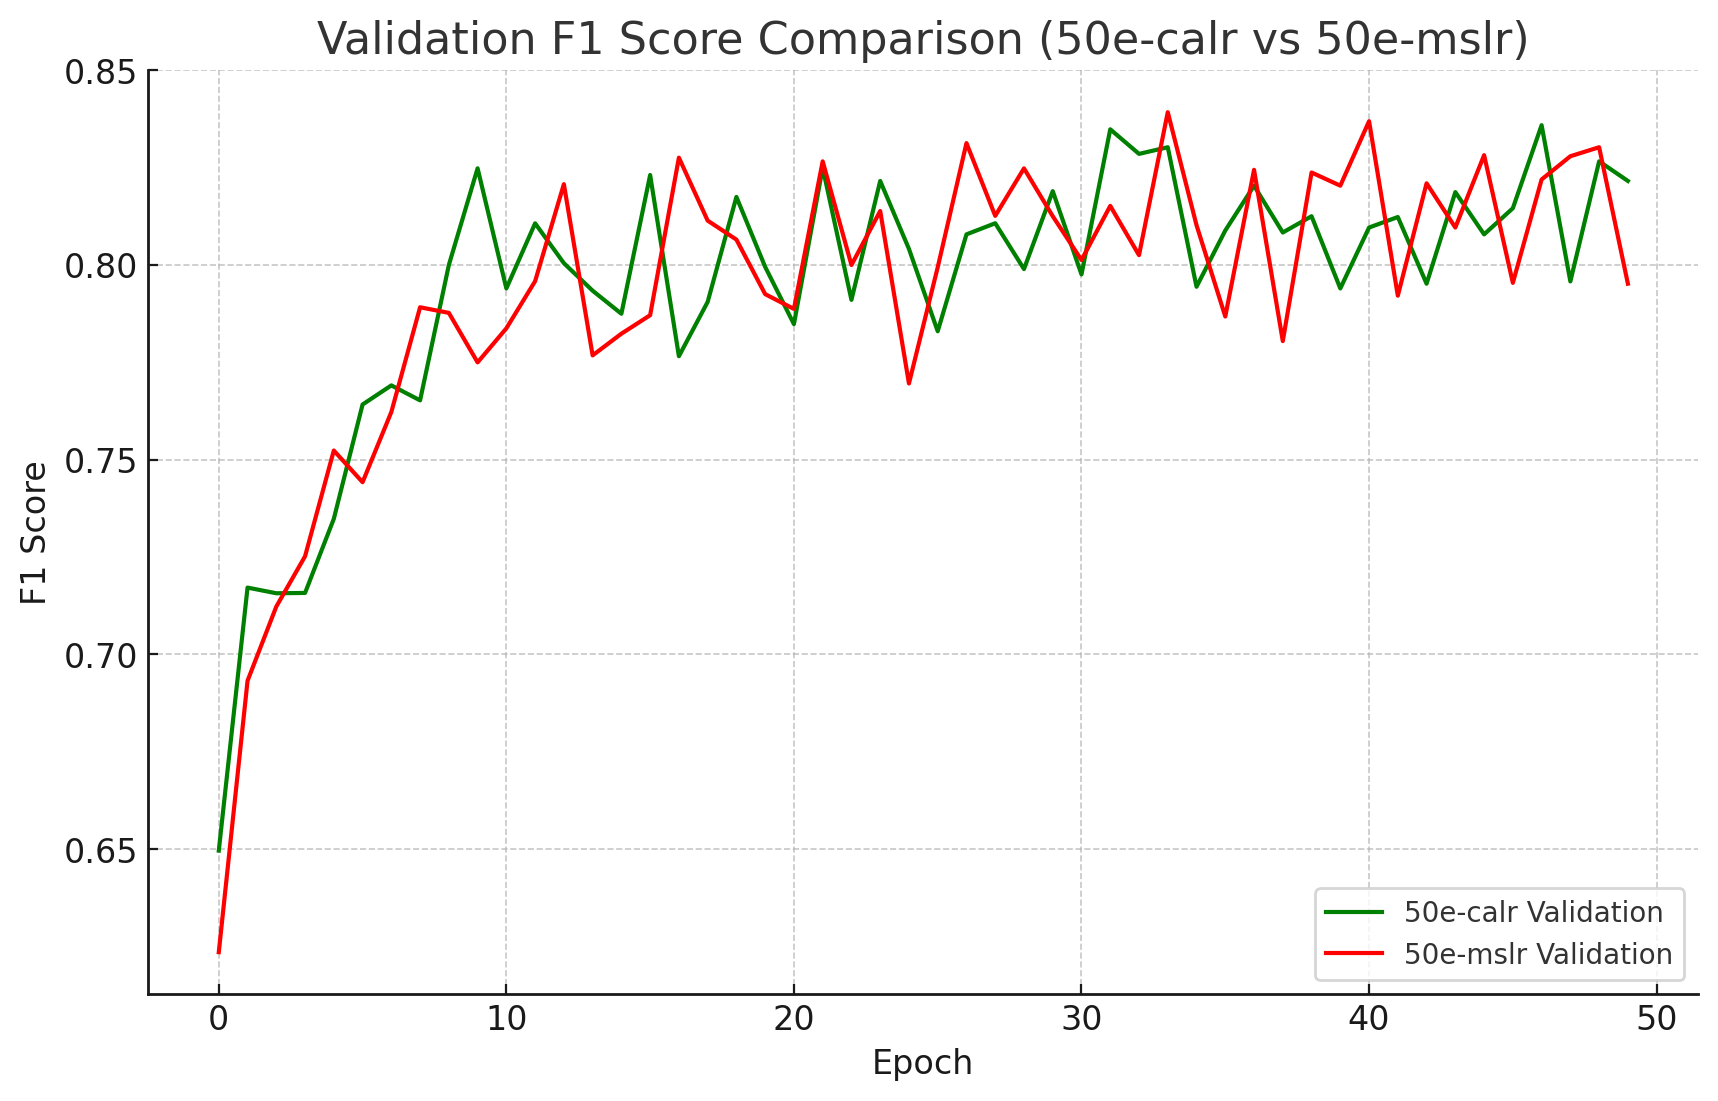
\includegraphics[width=\textwidth]{gambar/bab4-val-f1-score-50e.png}
    \caption{\emph{F1 Score} (\emph{validation}) - 50 \emph{epoch}}
  \end{subfigure}
  \caption{Kurva \emph{F1 Score} selama proses pelatihan model SSD-MobileNetV2}
  \label{fig:f1_score_curves}
\end{figure}

\begin{figure}[htbp]
  \centering
  \begin{subfigure}{0.45\textwidth}
    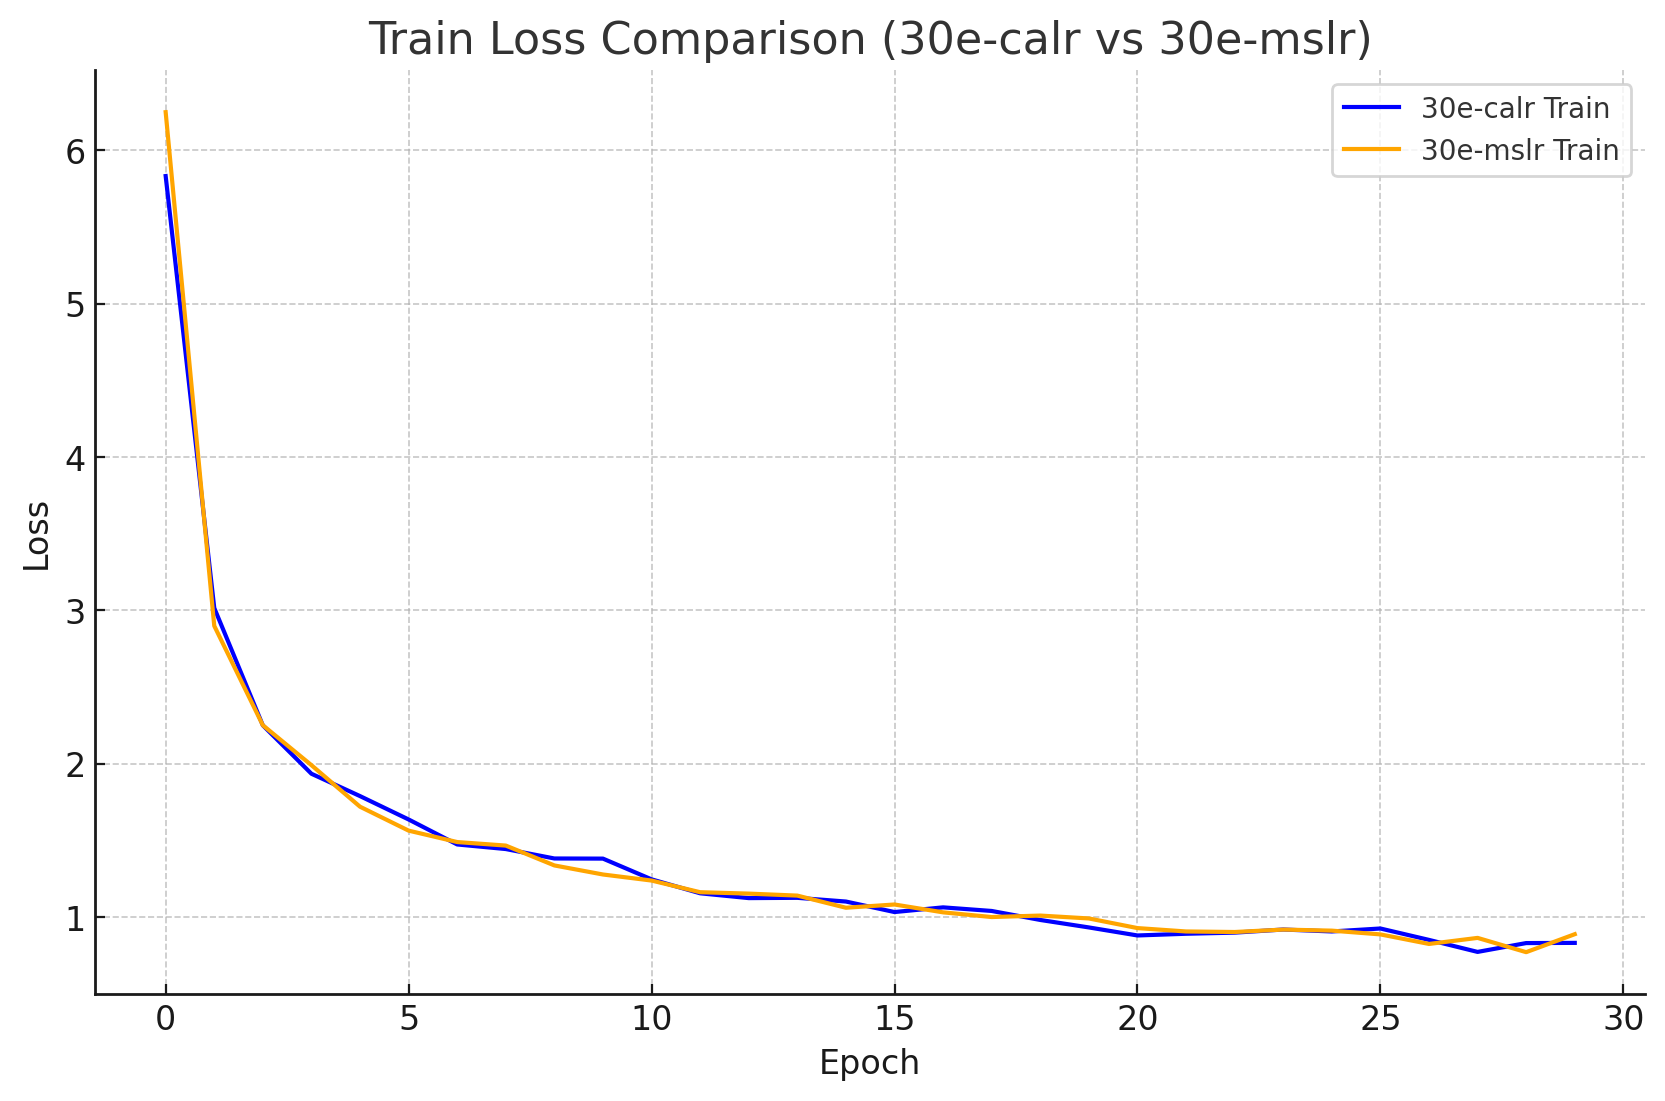
\includegraphics[width=\textwidth]{gambar/bab4-train-loss-30e.png}
    \caption{\emph{Loss} (\emph{training}) - 30 \emph{epoch}}
  \end{subfigure}
  \hfill
  \begin{subfigure}{0.45\textwidth}
    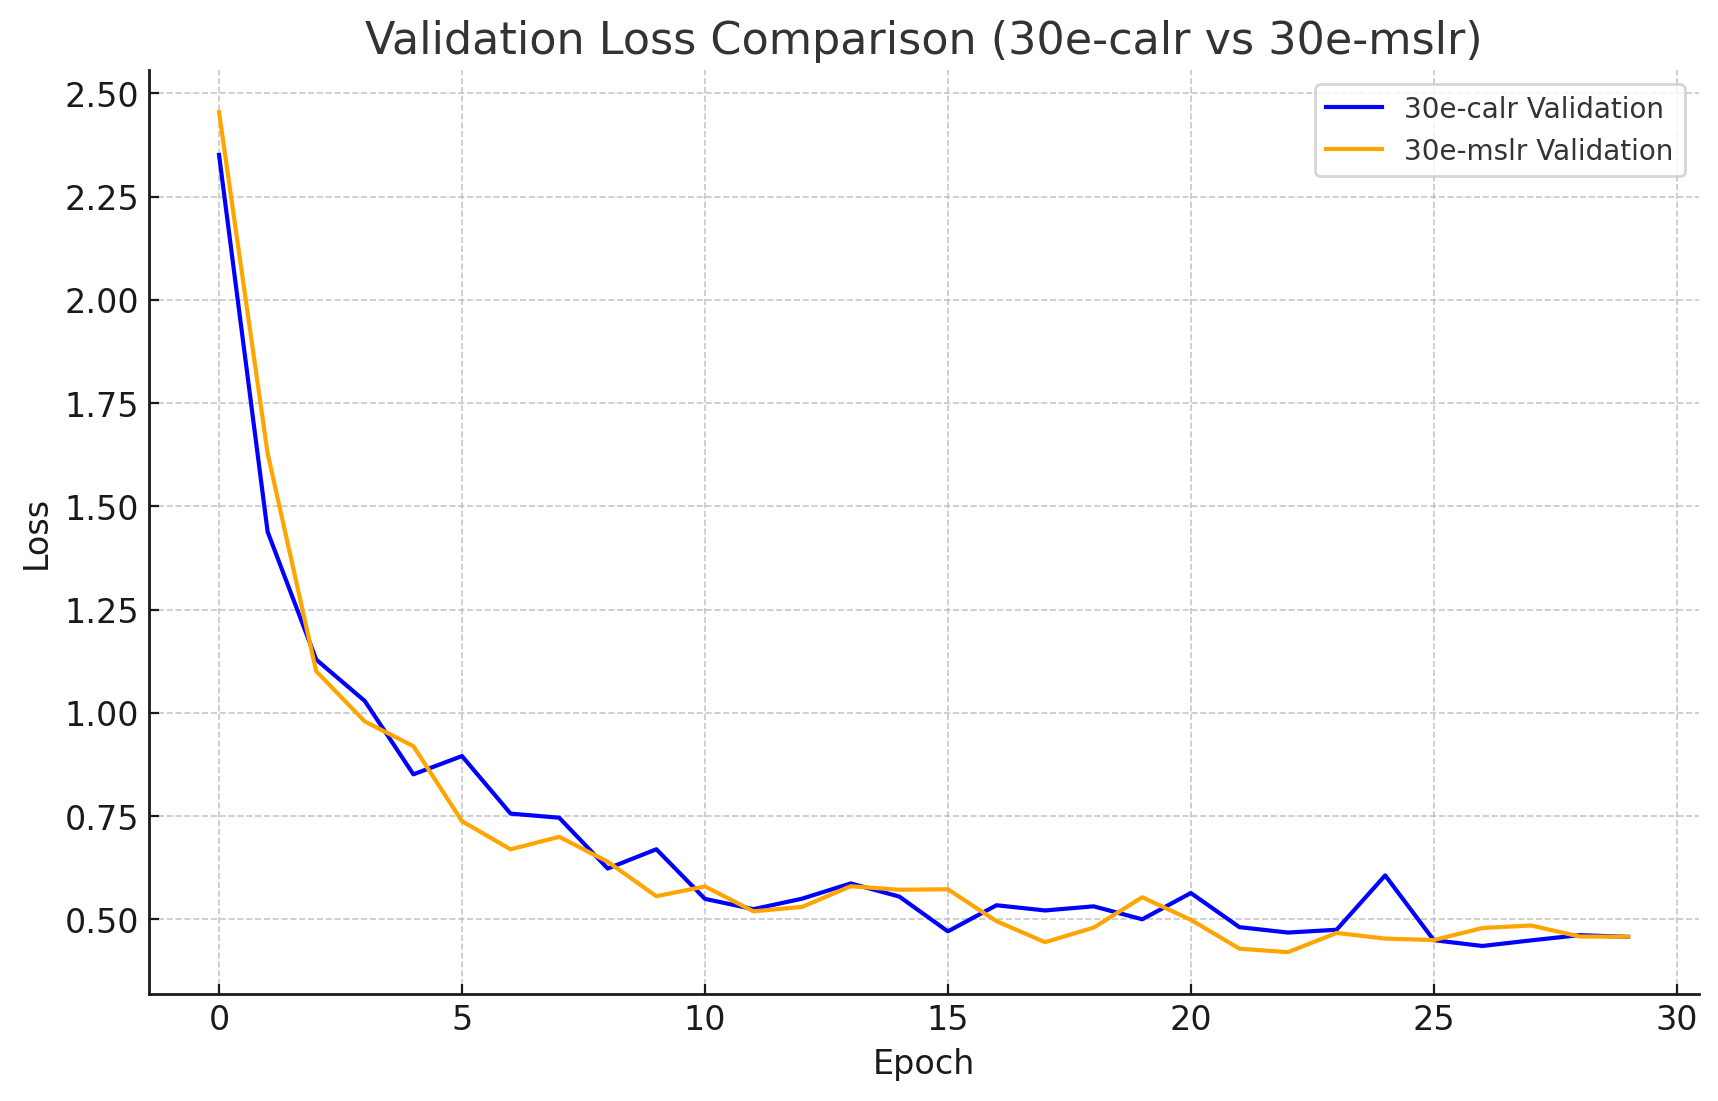
\includegraphics[width=\textwidth]{gambar/bab4-val-loss-30e.png}
    \caption{\emph{Loss} (\emph{validation}) - 30 \emph{epoch}}
  \end{subfigure}
  \hfill
  \begin{subfigure}{0.45\textwidth}
    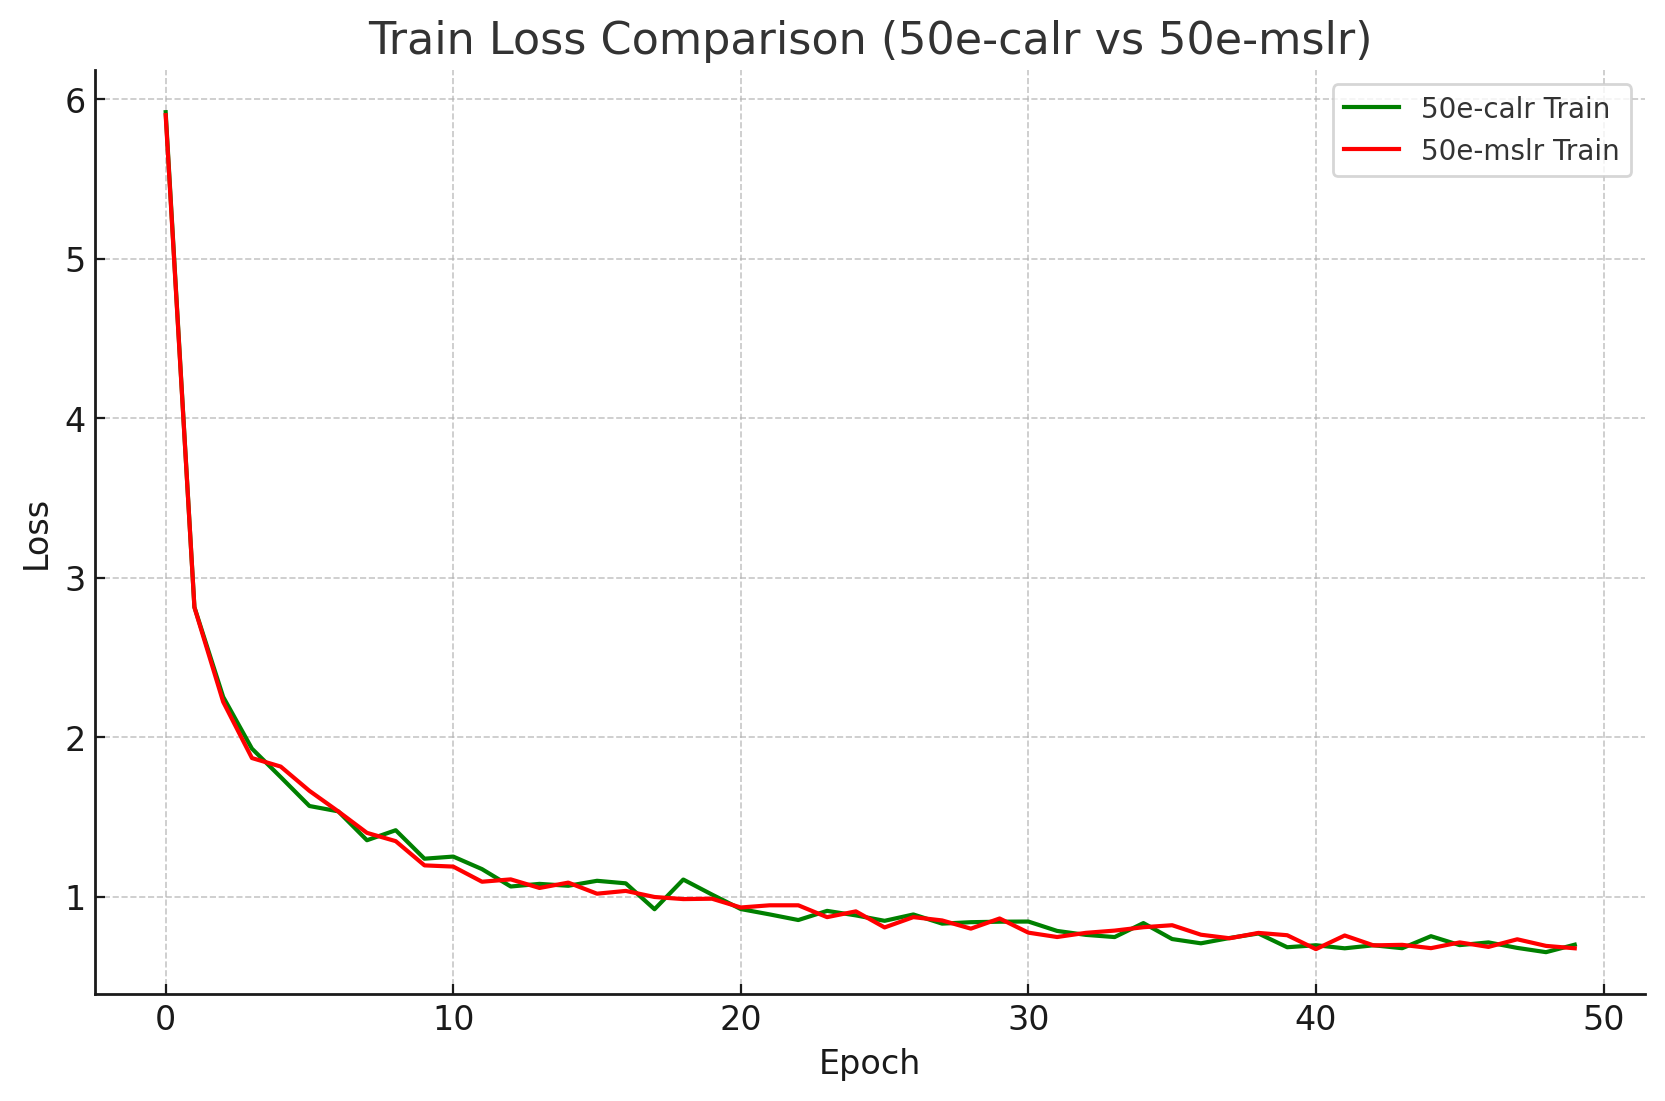
\includegraphics[width=\textwidth]{gambar/bab4-train-loss-50e.png}
    \caption{\emph{Loss} (\emph{training}) - 50 \emph{epoch}}
  \end{subfigure}
  \hfill
  \begin{subfigure}{0.45\textwidth}
    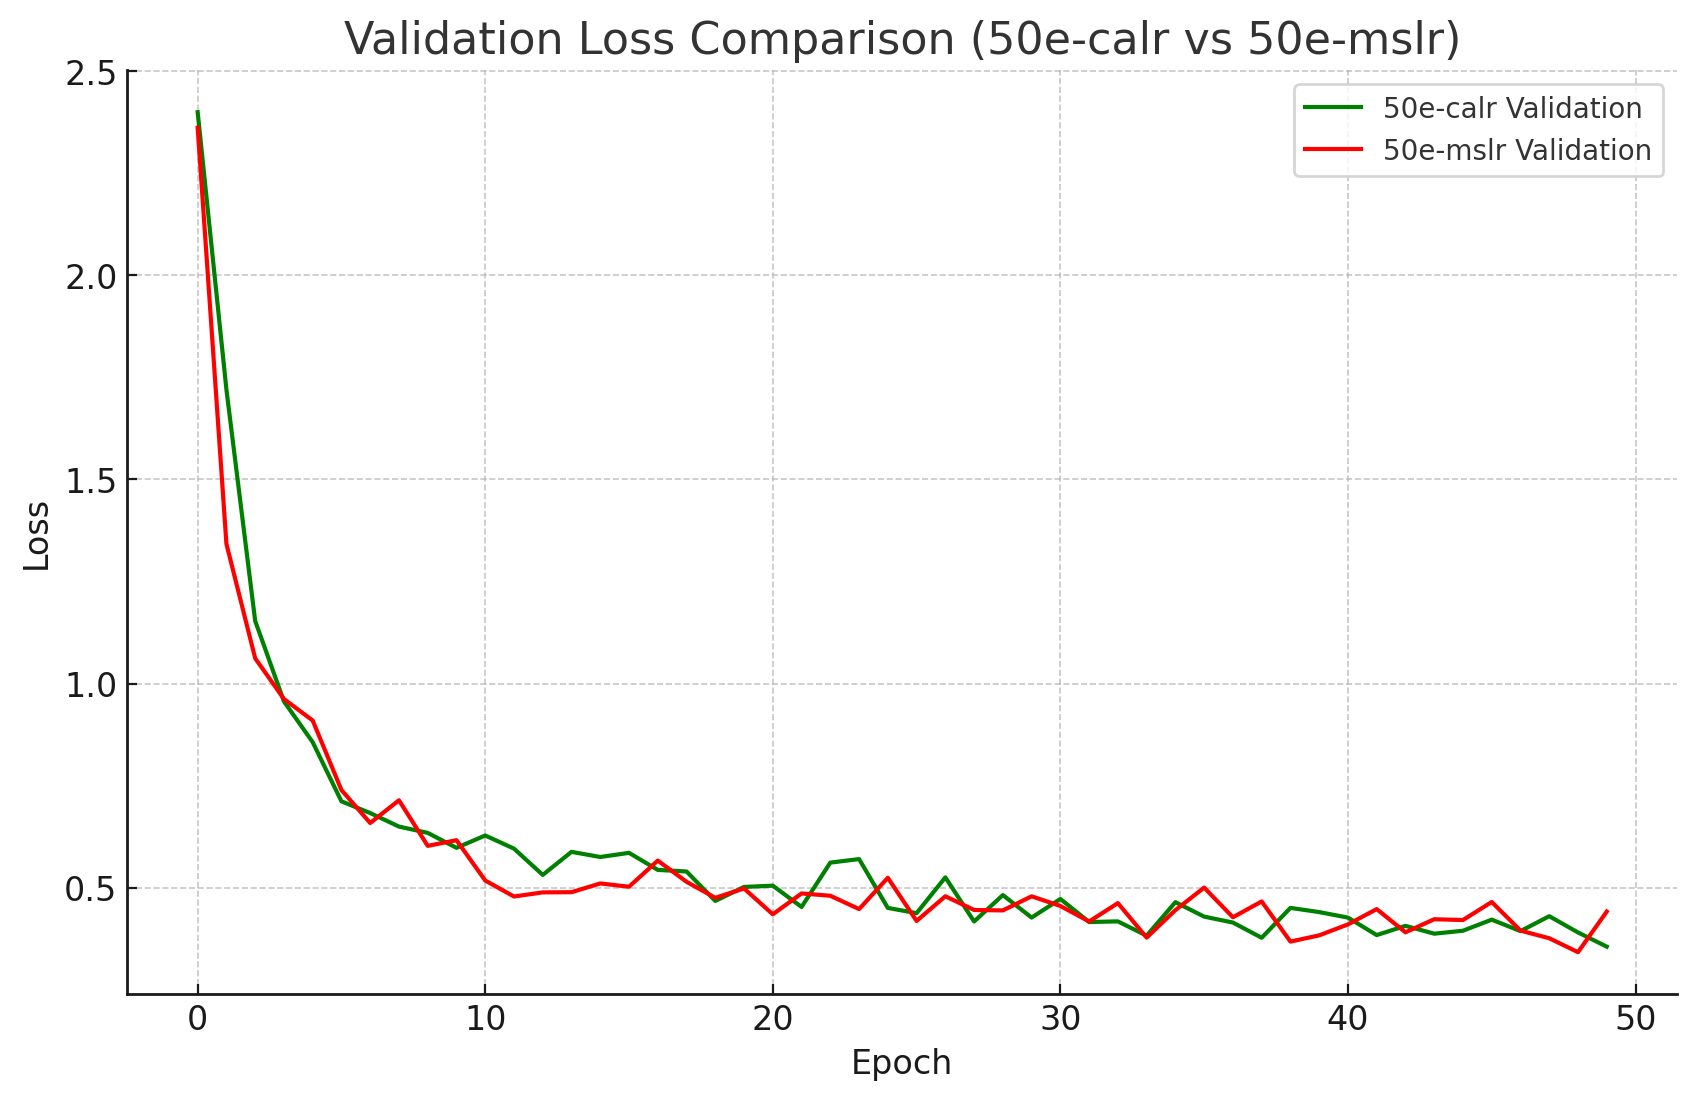
\includegraphics[width=\textwidth]{gambar/bab4-val-loss-50e.png}
    \caption{\emph{Loss} (\emph{validation}) - 50 \emph{epoch}}
  \end{subfigure}
  \caption{Kurva \emph{Loss} selama proses pelatihan model SSD-MobileNetV2}
  \label{fig:loss_curves}
\end{figure}

\begin{figure}[htbp]
  \centering
  \begin{subfigure}{0.45\textwidth}
    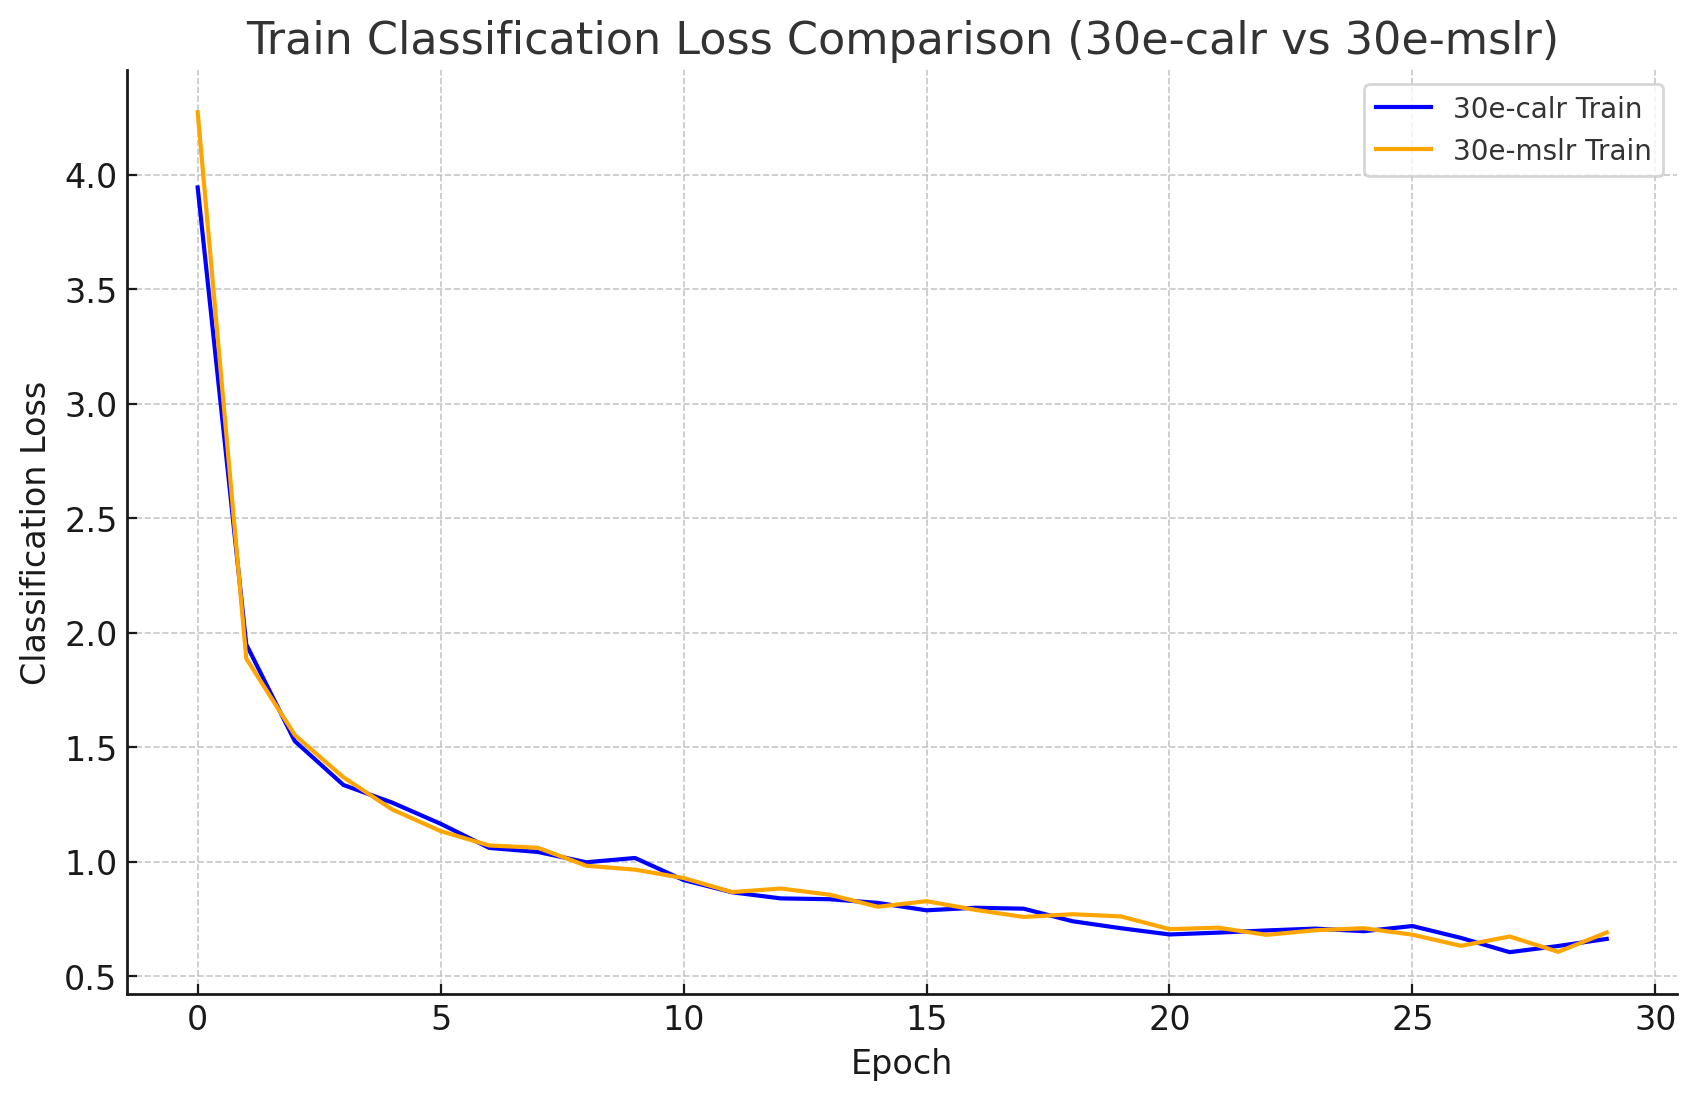
\includegraphics[width=\textwidth]{gambar/bab4-train-clsloss-30e.png}
    \caption{\emph{Classification Loss} (\emph{training}) - 30 \emph{epoch}}
  \end{subfigure}
  \hfill
  \begin{subfigure}{0.45\textwidth}
    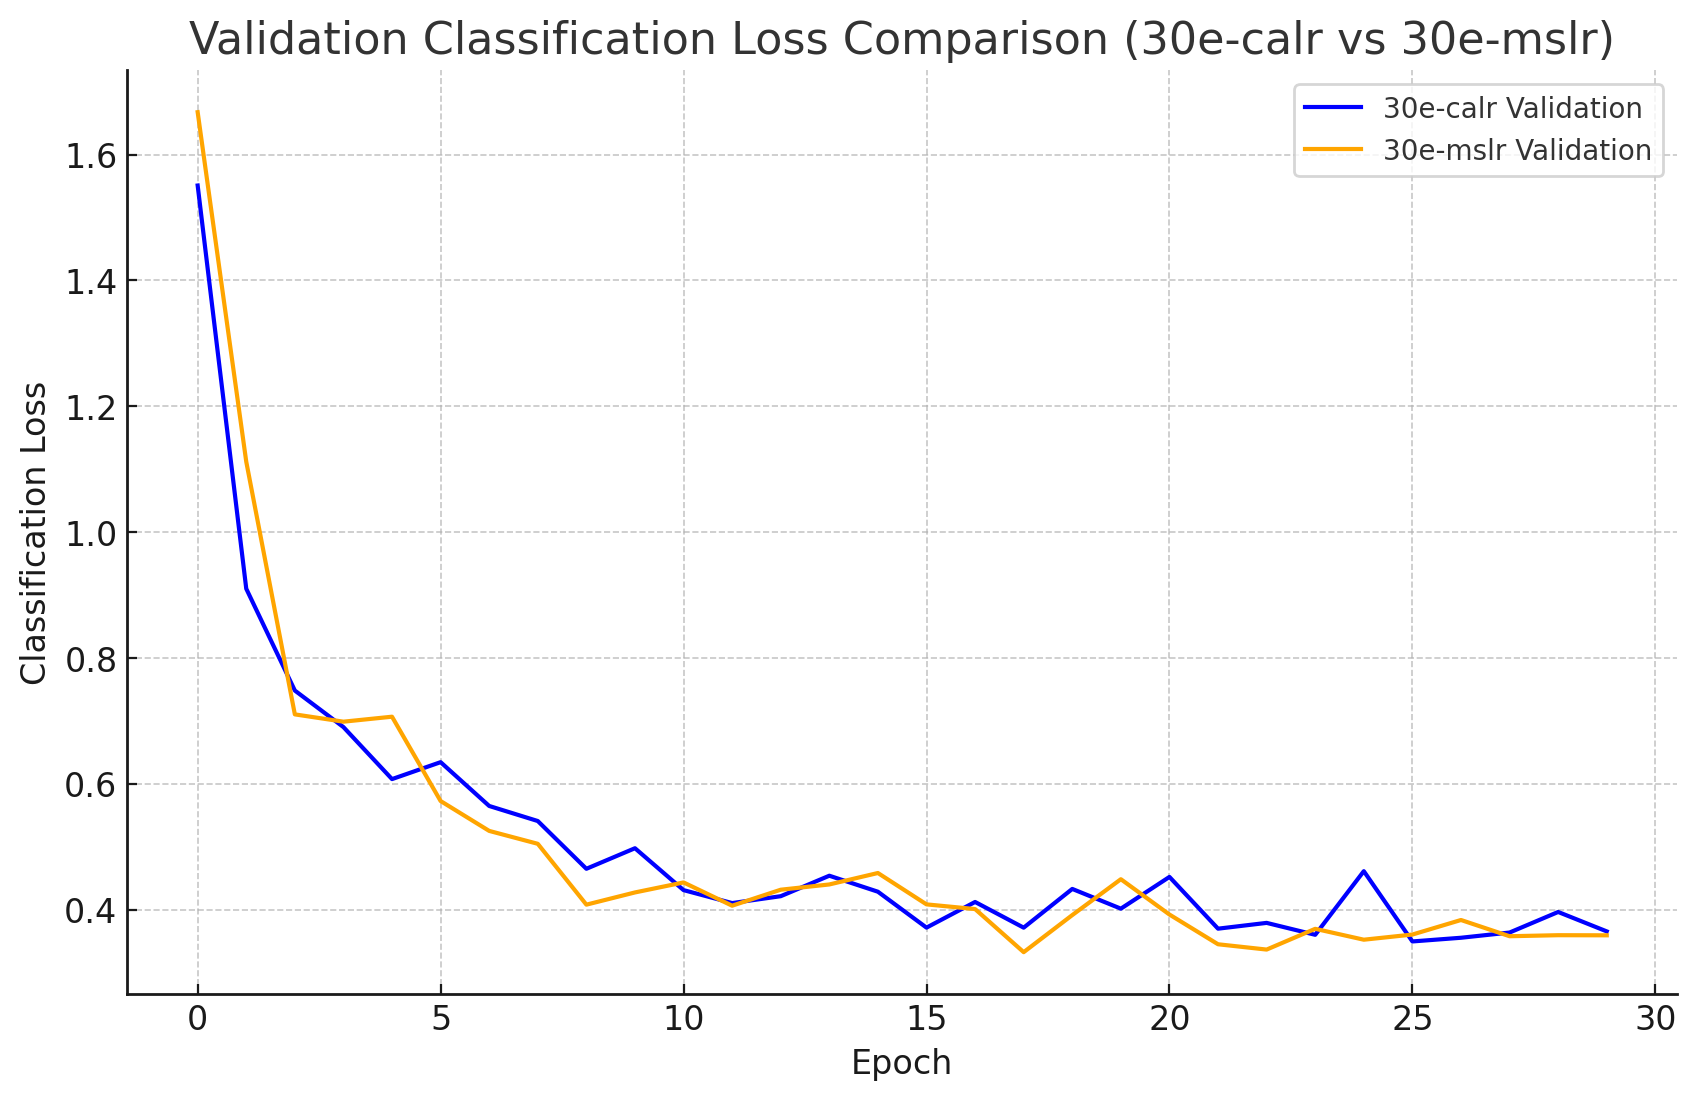
\includegraphics[width=\textwidth]{gambar/bab4-val-clsloss-30e.png}
    \caption{\emph{Classification Loss} (\emph{validation}) - 30 \emph{epoch}}
  \end{subfigure}
  \hfill
  \begin{subfigure}{0.45\textwidth}
    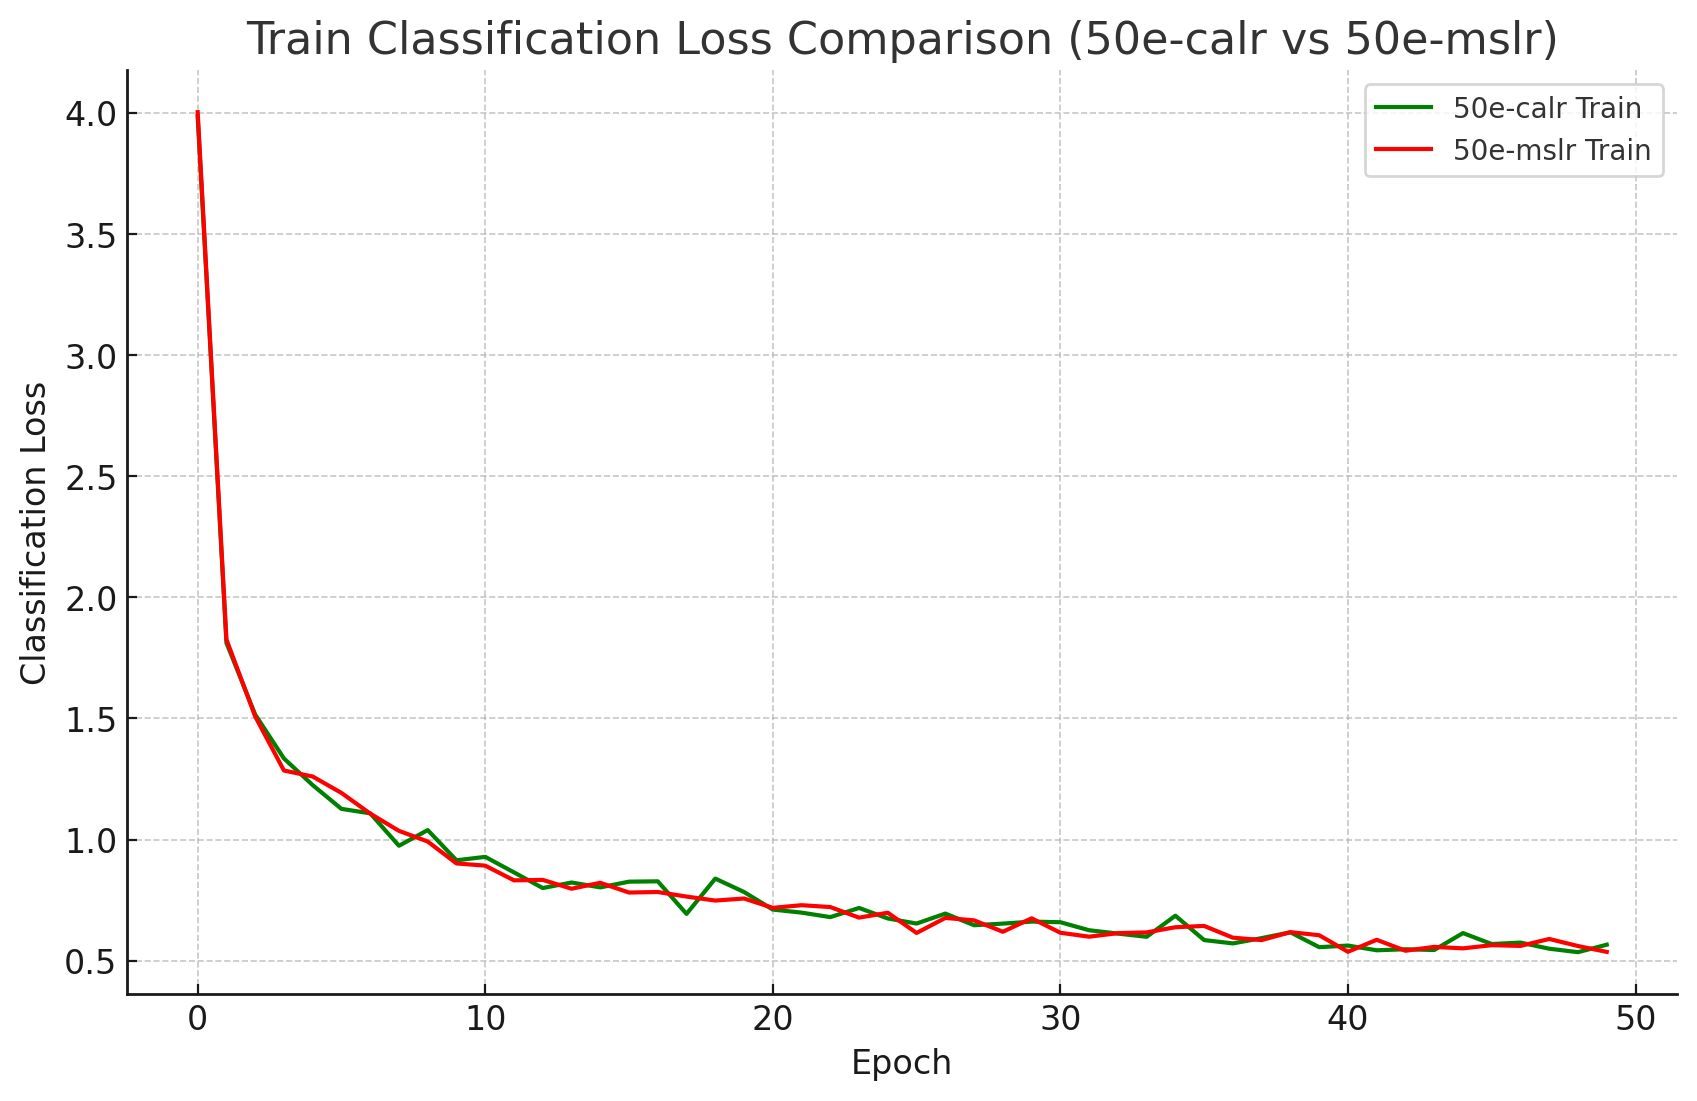
\includegraphics[width=\textwidth]{gambar/bab4-train-clsloss-50e.png}
    \caption{\emph{Classification Loss} (\emph{training}) - 50 \emph{epoch}}
  \end{subfigure}
  \hfill
  \begin{subfigure}{0.45\textwidth}
    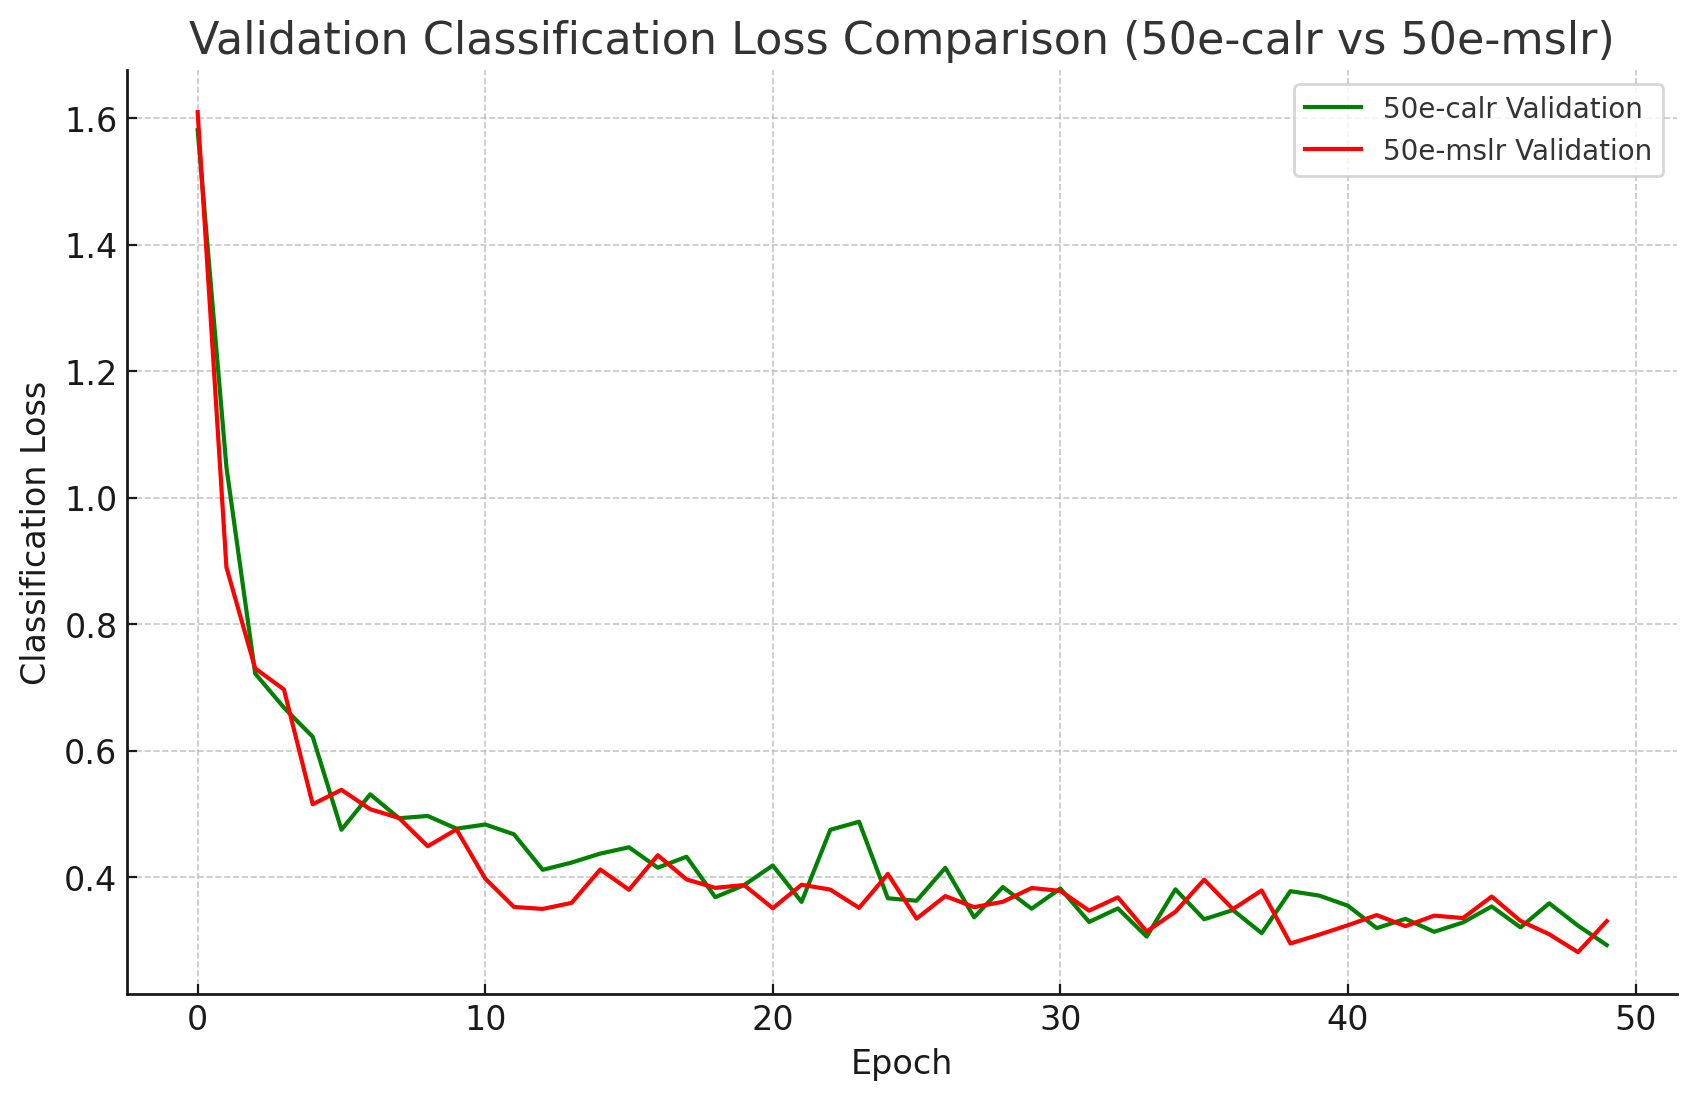
\includegraphics[width=\textwidth]{gambar/bab4-val-clsloss-50e.png}
    \caption{\emph{Classification Loss} (\emph{validation}) - 50 \emph{epoch}}
  \end{subfigure}
  \caption{Kurva \emph{Classification Loss} selama proses pelatihan model SSD-MobileNetV2}
  \label{fig:classification_loss_curves}
\end{figure}

\begin{figure}[htbp]
  \centering
  \begin{subfigure}{0.45\textwidth}
    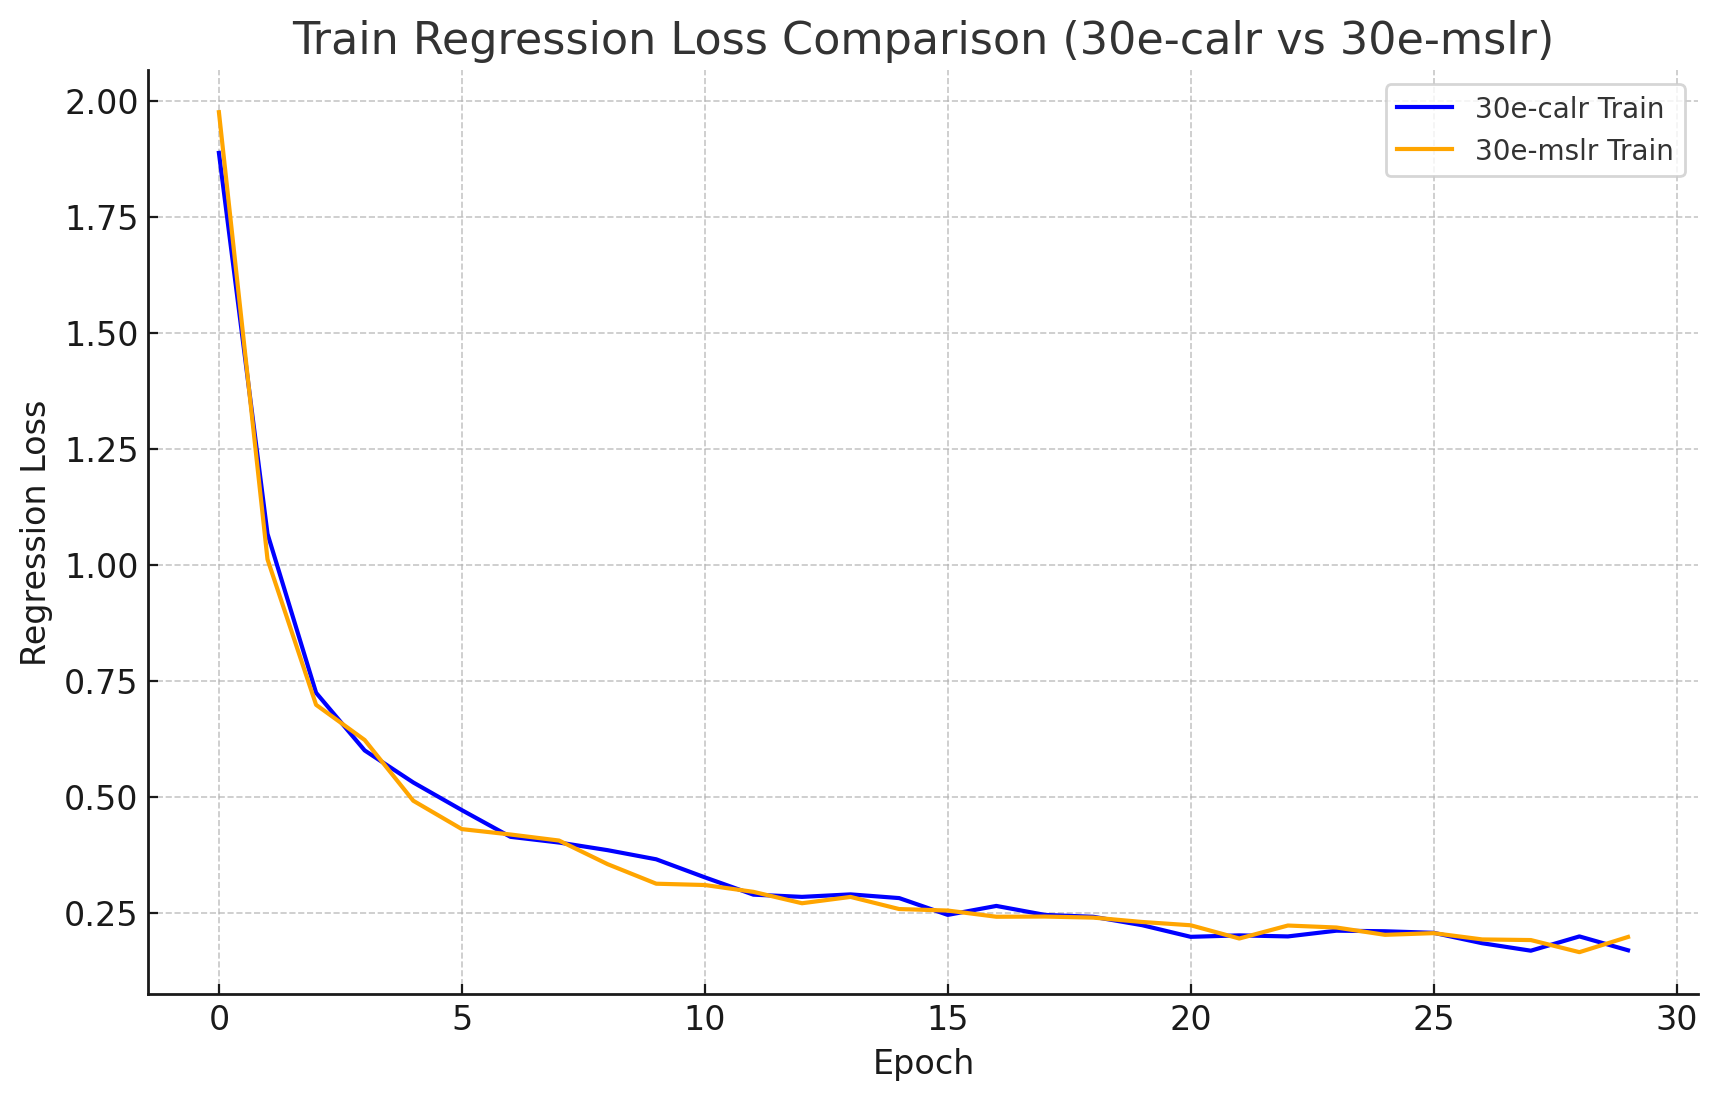
\includegraphics[width=\textwidth]{gambar/bab4-train-regloss-30e.png}
    \caption{\emph{Regression Loss} (\emph{training}) - 30 \emph{epoch}}
  \end{subfigure}
  \hfill
  \begin{subfigure}{0.45\textwidth}
    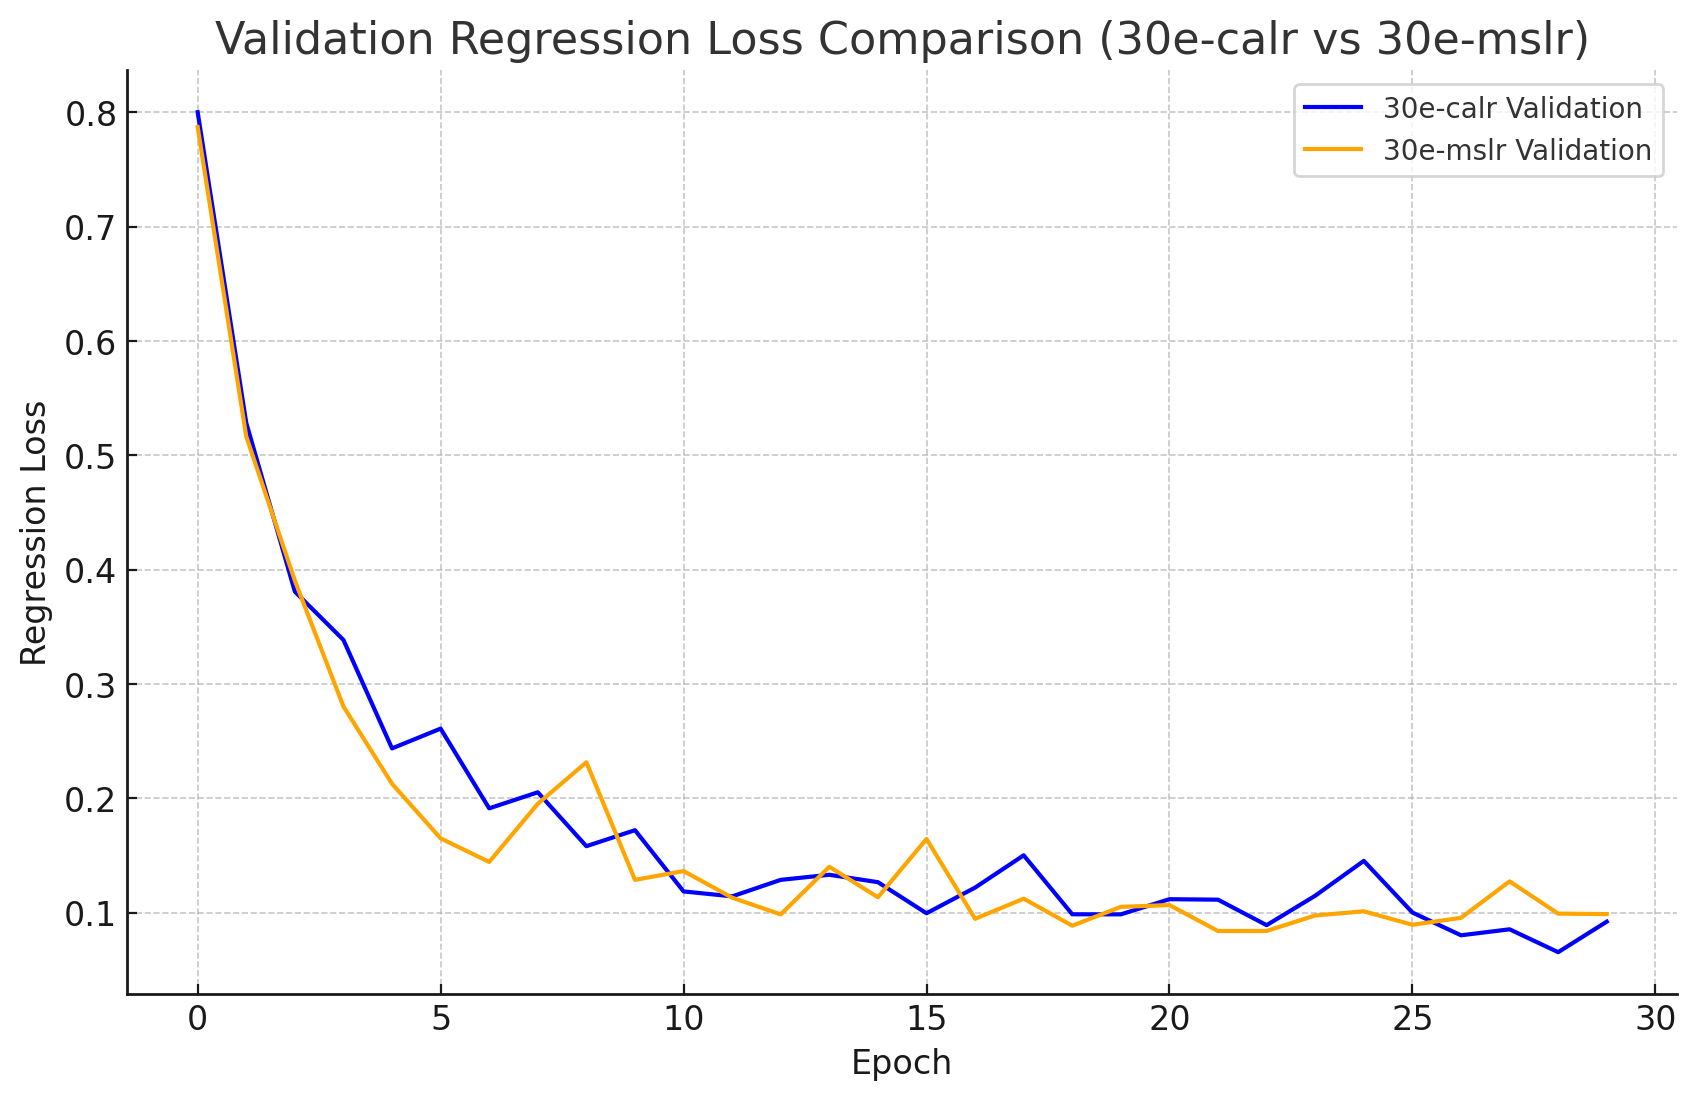
\includegraphics[width=\textwidth]{gambar/bab4-val-regloss-30e.png}
    \caption{\emph{Regression Loss} (\emph{validation}) - 30 \emph{epoch}}
  \end{subfigure}
  \hfill
  \begin{subfigure}{0.45\textwidth}
    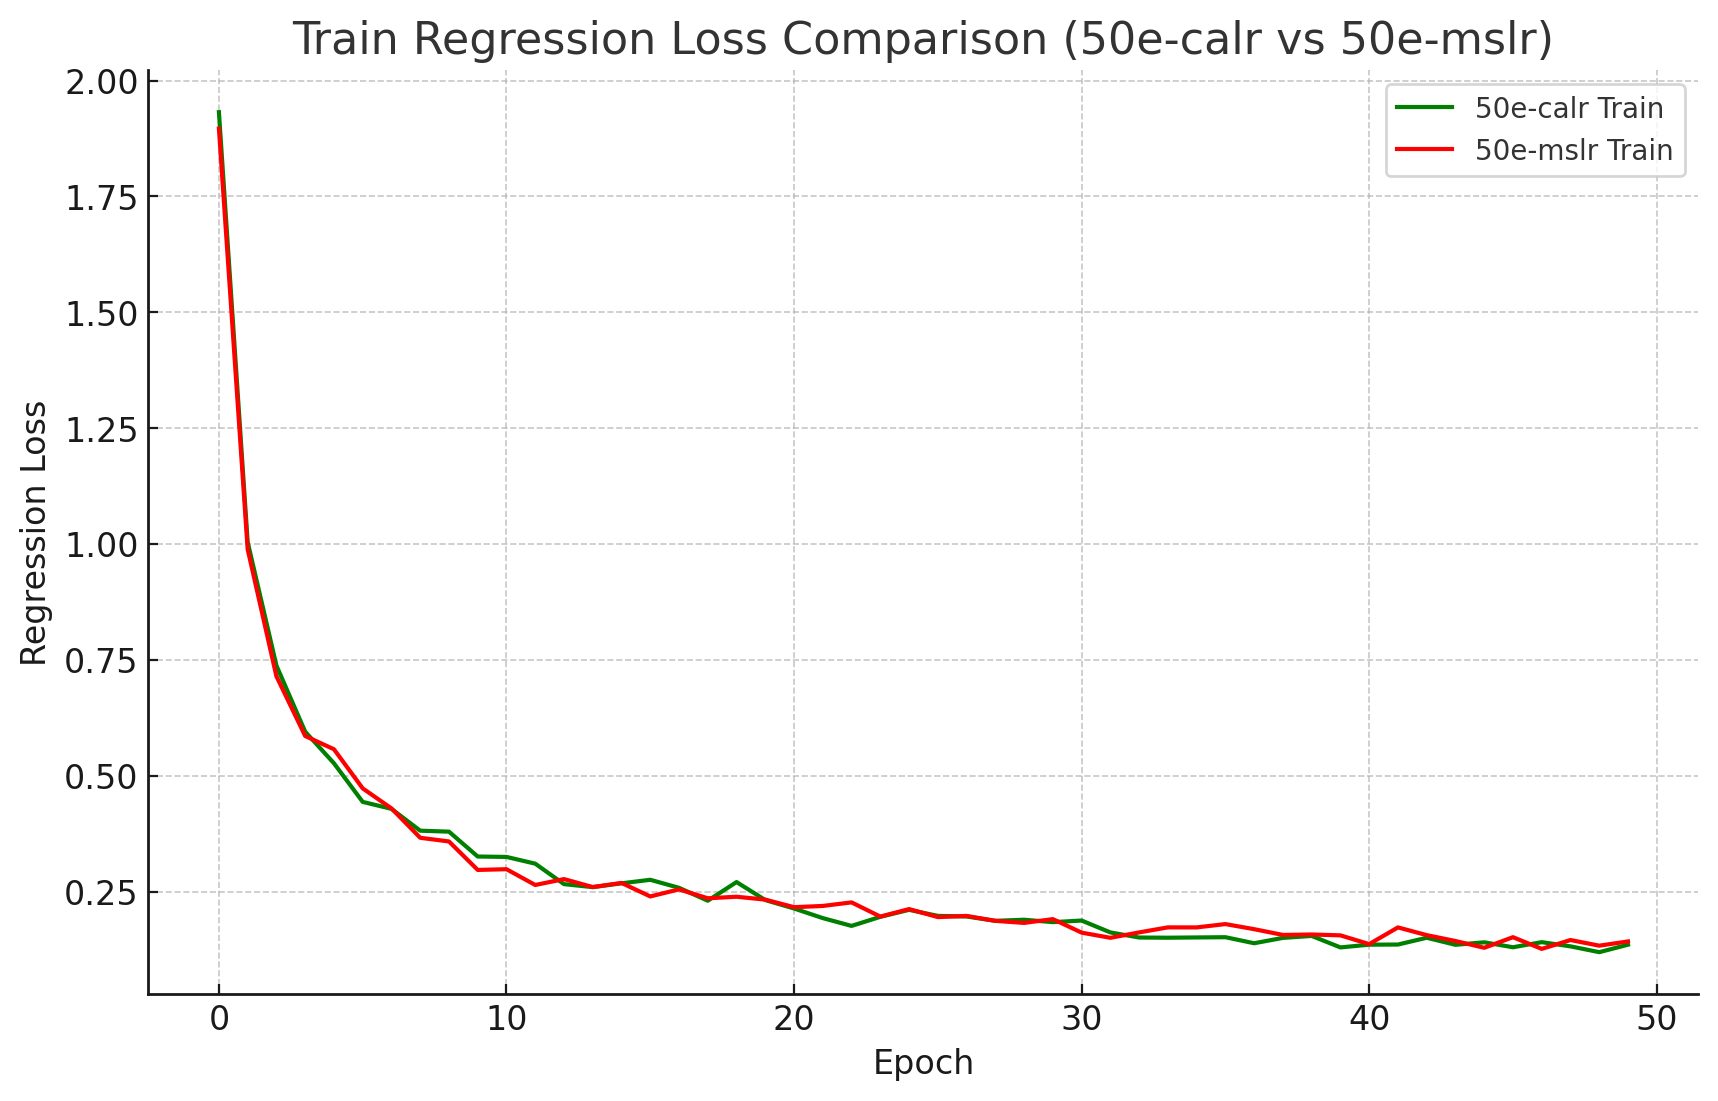
\includegraphics[width=\textwidth]{gambar/bab4-train-regloss-50e.png}
    \caption{\emph{Regression Loss} (\emph{training}) - 50 \emph{epoch}}
  \end{subfigure}
  \hfill
  \begin{subfigure}{0.45\textwidth}
    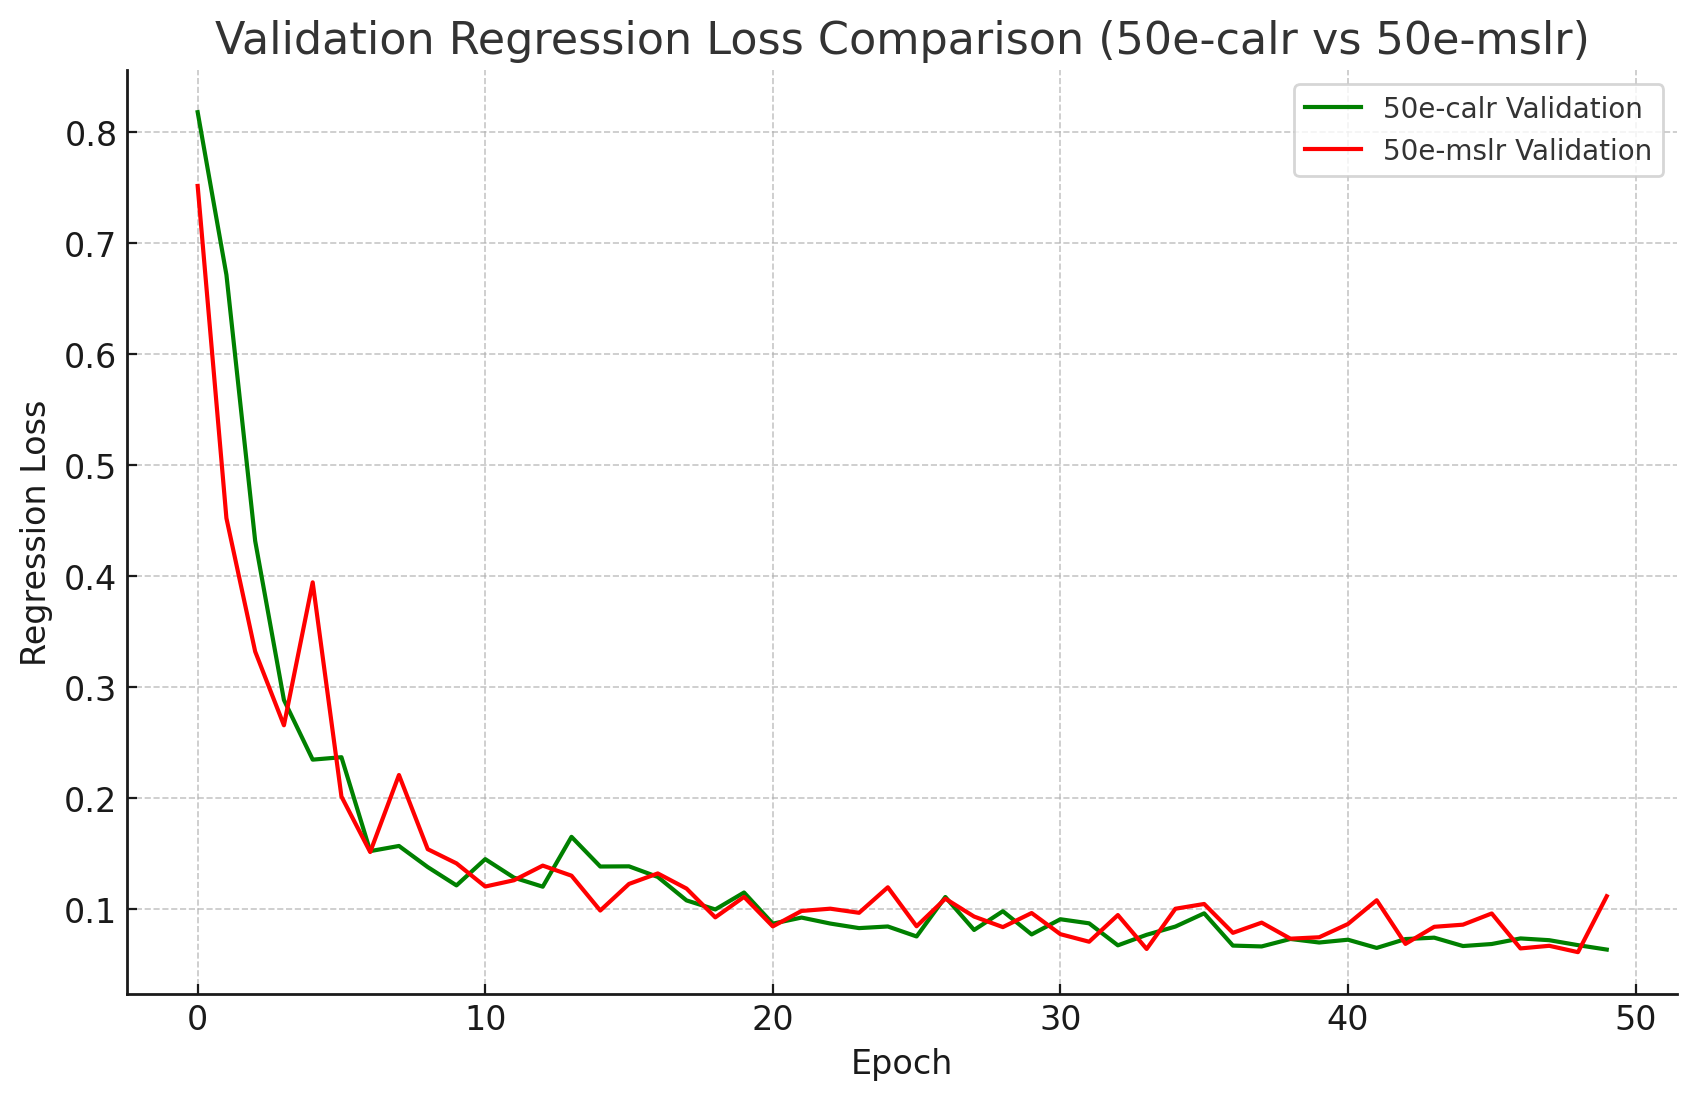
\includegraphics[width=\textwidth]{gambar/bab4-val-regloss-50e.png}
    \caption{\emph{Regression Loss} (\emph{validation}) - 50 \emph{epoch}}
  \end{subfigure}
  \caption{Kurva \emph{Regression Loss} selama proses pelatihan model SSD-MobileNetV2}
  \label{fig:regression_loss_curves}
\end{figure}      

Berdasarkan grafik yang ditampilkan pada Gambar \ref{fig:accuracy_curves} (\emph{accuracy}), \ref{fig:precision_curves} (\emph{precision}), \ref{fig:recall_curves} (\emph{recall}), \ref{fig:f1_score_curves} (\emph{F1 score}), \ref{fig:loss_curves} (\emph{loss}), \ref{fig:classification_loss_curves} (\emph{classification loss}), dan \ref{fig:regression_loss_curves} (\emph{regression loss}), dapat dianalisis hasil pelatihan dari empat konfigurasi model yang berbeda, yaitu 30 \emph{epoch} dengan \emph{scheduler} \emph{CosineAnnealingLR}, 30 \emph{epoch} dengan \emph{scheduler} \emph{MultiStepLR}, 50 \emph{epoch} dengan \emph{scheduler} \emph{CosineAnnealingLR}, dan 50 \emph{epoch} dengan \emph{scheduler} \emph{MultiStepLR}.

Secara umum, tren yang terlihat pada grafik adalah penurunan loss yang stabil dan akurasi yang meningkat seiring dengan penambahan \emph{epoch}. Namun, terdapat beberapa perbedaan yang mencolok antara konfigurasi yang satu dengan yang lainnya.

\subsubsection{30 \emph{epoch} dengan \emph{CosineAnnealingLR} vs \emph{MultiStepLR}}

Pada grafik \ref{fig:accuracy_curves}, terlihat bahwa konfigurasi 30 \emph{epoch} dengan \emph{CosineAnnealingLR} (\emph{30e-calr}) menunjukkan peningkatan \emph{accuracy} yang lebih cepat dibandingkan dengan konfigurasi 30 \emph{epoch} dengan \emph{MultiStepLR} (\emph{30e-mslr}) pada awal pelatihan. Namun, setelah mencapai titik tertentu, kedua konfigurasi tersebut mulai mendekati hasil yang serupa pada \emph{epoch} akhir. 

Pada grafik \ref{fig:loss_curves}, kita juga dapat melihat bahwa \emph{30e-calr} cenderung memiliki penurunan \emph{loss} yang lebih stabil, sementara \emph{30e-mslr} menunjukkan fluktuasi yang lebih besar terutama pada \emph{epoch} awal. Meskipun demikian, kedua konfigurasi mengalami penurunan \emph{loss} yang cukup signifikan sepanjang pelatihan.

\subsubsection{50 \emph{epoch} dengan \emph{CosineAnnealingLR} vs \emph{MultiStepLR}}

Untuk konfigurasi 50 \emph{epoch}, pada grafik \ref{fig:accuracy_curves} dan \ref{fig:loss_curves}, terlihat bahwa konfigurasi 50 \emph{epoch} dengan \emph{CosineAnnealingLR} (\emph{50e-calr}) dan \emph{50e-mslr} menunjukkan tren yang lebih stabil dibandingkan dengan konfigurasi 30 \emph{epoch}. Pada grafik \ref{fig:classification_loss_curves}, dapat dilihat bahwa kedua konfigurasi ini menunjukkan penurunan yang lebih konsisten pada \emph{loss} klasifikasi. Meskipun pada awalnya \emph{50e-mslr} sedikit lebih tinggi, namun seiring berjalannya waktu, keduanya menunjukkan hasil yang hampir serupa.

Namun, \emph{50e-calr} menunjukkan keuntungan dalam hal peningkatan akurasi yang lebih cepat pada \emph{epoch} awal dibandingkan \emph{50e-mslr}, seperti yang terlihat pada grafik \ref{fig:accuracy_curves}.

\subsubsection{Perbandingan antara 30 \emph{epoch} dan 50 \emph{epoch}}

Ketika membandingkan antara konfigurasi 30 \emph{epoch} dan 50 \emph{epoch}, dapat dilihat bahwa secara umum, 50 \emph{epoch} memberikan hasil yang lebih stabil pada berbagai metrik, termasuk \emph{accuracy}, \emph{loss}, dan \emph{F1 score}. Hal ini dikarenakan lebih banyak \emph{epoch} memberikan kesempatan bagi model untuk lebih menyempurnakan hasilnya.

Namun, untuk beberapa konfigurasi, seperti \emph{30e-calr}, meskipun hasilnya lebih cepat tercapai pada \emph{epoch} yang lebih sedikit, model dengan 50 \emph{epoch} masih memberikan hasil yang lebih baik dalam hal generalisasi, sebagaimana tercermin dari Gambar \ref{fig:recall_curves} (\emph{recall}) dan \ref{fig:f1_score_curves} (\emph{F1 score}).

Berdasarkan analisis dari grafik-grafik yang ada, dapat disimpulkan bahwa secara keseluruhan, konfigurasi dengan \emph{epoch} lebih banyak (50 \emph{epoch}) cenderung memberikan hasil yang lebih stabil dan lebih baik dalam hal \emph{accuracy}, \emph{loss}, \emph{F1 score}, \emph{precision}, \emph{recall}, dan \emph{regression loss}. Namun, konfigurasi 30 \emph{epoch} dengan \emph{scheduler} \emph{CosineAnnealingLR} (\emph{30e-calr}) menunjukkan hasil yang cukup cepat pada \emph{epoch} awal, namun tidak sebaik \emph{50e-calr} dalam jangka panjang. Meskipun demikian, pemilihan antara konfigurasi 30 atau 50 \emph{epoch} bergantung pada kebutuhan spesifik dan waktu pelatihan yang tersedia.

\subsection{Evaluasi Model}

Evaluasi model dilakukan pada dataset validasi untuk menilai kemampuan generalisasi model dalam mendeteksi objek yang belum pernah dilihat sebelumnya

Suatu truk dikatakan overdimensi jika memiliki label \emph{overdimension} dan \emph{truck}. Namun, suatu truk dikatakan bukan overdimensi jika memiliki label \emph{truck} saja. Sehingga terjadi beberapa penyesuaian dalam perhitungan mAP. Dimana awalnya terdapat 3 AP (untuk kelas \emph{car}, \emph{truck}, dan \emph{overdimension}), namun setelah penyesuaian, hanya terdapat 2 AP (untuk kelas \emph{normal} dan \emph{overdimension}) karena tujuan \emph{car} dilabel hanya agar model dapat memahami bahwa \emph{car} bukan termasuk \emph{truck}.

Perhitungan mAP untuk model terbaik (50 \emph{epoch} dengan \emph{CosineAnnealingLR}) dilakukan menggunakan rumus mAP pada Persamaan \ref{eq:mAP}.

\begin{itemize}[nolistsep]
  \item Kelas Normal: $\mbox{AP}_{\mbox{normal}} = 0.879$
  \item Kelas Overdimension: $\mbox{AP}_{\mbox{overdimension}} = 0.732$
\end{itemize}

Dari hasil evaluasi untuk model dengan konfigurasi terbaik, diperoleh nilai mAP sebesar 0.805, dengan rincian AP untuk setiap kelas sebagai berikut:

\begin{table}[htbp]
  \centering
  \caption{Hasil evaluasi model SSD-MobileNetV2 berdasarkan Average Precision}
  \label{tab:ap_results}
  \begin{tabular}{|l|c|}
    \hline
    \rowcolor[HTML]{C0C0C0}
    \textbf{Kelas} & \textbf{Average Precision (AP)} \\
    \hline
    Normal & 0.879 \\
    \hline
    Overdimension & 0.732 \\
    \hline
    \textbf{Mean Average Precision (mAP)} & \textbf{0.805} \\
    \hline
  \end{tabular}
\end{table}

Dari Tabel \ref{tab:ap_results}, dapat diamati bahwa model menunjukkan performa yang sangat baik dalam mendeteksi kelas 'normal' dan 'overdimension' dengan AP mencapai nilai ideal 0.879 dan 0.732. 

Perbandingan hasil pelatihan untuk berbagai konfigurasi menunjukkan bahwa model dengan 50 \emph{epoch} dan \emph{scheduler} \emph{CosineAnnealingLR} memberikan performa terbaik. \emph{CosineAnnealingLR} memungkinkan model untuk melakukan eksplorasi learning rate secara adaptif, sehingga membantu model mencapai konvergensi yang lebih baik dan menghindari jebakan lokal minimum.

\begin{table}[htbp]
  \centering
  \caption{Perbandingan mAP untuk berbagai konfigurasi pelatihan}
  \label{fig:map_comparison}
  \begin{tabular}{|l|c|}
    \hline
    \rowcolor[HTML]{C0C0C0}
    \textbf{Konfigurasi} & \textbf{mAP} \\
    \hline
    30 epoch dengan CosineAnnealingLR & 0.802 \\
    \hline
    30 epoch dengan MultiStepLR & 0.798 \\
    \hline
    \textbf{50 epoch dengan CosineAnnealingLR} & \textbf{0.805} \\
    \hline
    50 epoch dengan MultiStepLR & 0.763 \\
    \hline
  \end{tabular}
\end{table}

Hasil evaluasi ini menunjukkan bahwa model SSD-MobileNetV2 yang dilatih memiliki kemampuan yang baik dalam mendeteksi dan mengklasifikasikan kendaraan, terutama untuk kelas 'truck' dan 'overdimension'. Untuk meningkatkan performa deteksi kendaraan overdimensi, beberapa strategi yang dapat diterapkan antara lain menambah jumlah sampel untuk kelas tersebut, melakukan augmentasi data yang lebih intensif, atau menggunakan teknik transfer learning yang lebih optimal.

\section{Pembahasan Hasil Eksperimen}
\label{sec:pembahasanhasileksperimen}

Berdasarkan hasil pengujian yang telah dilakukan pada perangkat \emph{edge} dan transfer data ke \emph{cloud}, beberapa temuan penting dapat disajikan untuk mengevaluasi performa sistem deteksi kendaraan overdimensi secara keseluruhan.

\subsection{Eksperimen 1: Pengujian Model pada Perangkat \emph{Edge}}
\label{sec:eksperimen1}

Pengujian model pada perangkat \emph{edge} dilakukan untuk mengukur performa inferensi \emph{real-time} dalam mendeteksi dan mengklasifikasikan kendaraan yang melintas di gerbang tol. Model SSD-MobileNetV2 dengan format ONNX diimplementasikan pada kedua perangkat \emph{edge} dan diuji selama periode pengujian.

\subsubsection{Waktu Inferensi dan FPS}

Waktu inferensi dan FPS memiliki hubungan yang berbanding terbalik seperti yang sudah dijelaskan pada Persamaan \ref{eq:fps_inference_time}. Karena waktu inferensi diukur dalam milidetik, dan FPS diukur dalam frame per detik, maka FPS dapat dihitung dengan persamaan:

\begin{equation}
  \mbox{FPS} = \frac{1000}{\mbox{Waktu Inferensi}}
\end{equation}

Tabel \ref{tab:inference_time} menunjukkan perbandingan waktu inferensi dan FPS pada kedua perangkat dengan resolusi input 640x480.

\begin{table}[htbp]
  \centering
  \caption{Perbandingan waktu inferensi dan FPS pada perangkat \emph{edge}}
  \label{tab:inference_time}
  \setlength{\tabcolsep}{4pt}
  \small
  \begin{tabular}{|l|c|c|c|c|}
  \hline
  \rowcolor[HTML]{C0C0C0}
  \textbf{Perangkat} & \multicolumn{2}{c|}{\textbf{Waktu Inferensi (ms)}} & \multicolumn{2}{c|}{\textbf{FPS}} \\
  \cline{2-5}
  \rowcolor[HTML]{C0C0C0}
  & \textbf{Min} & \textbf{Max} & \textbf{Min} & \textbf{Max} \\
  \hline
  NVIDIA Jetson Nano 4GB & 20.87 & 36.27 & 27.57 & 47.93 \\
  \hline
  Beelink Gemini T34 & 238.10 & 3030.30 & 0.33 & 4.20 \\
  \hline
  \end{tabular}
\end{table}

Gambar \ref{fig:fps_over_time} menampilkan perbandingan performa FPS kedua perangkat selama 15 menit pengujian. 

\begin{figure}[htbp]
  \centering
  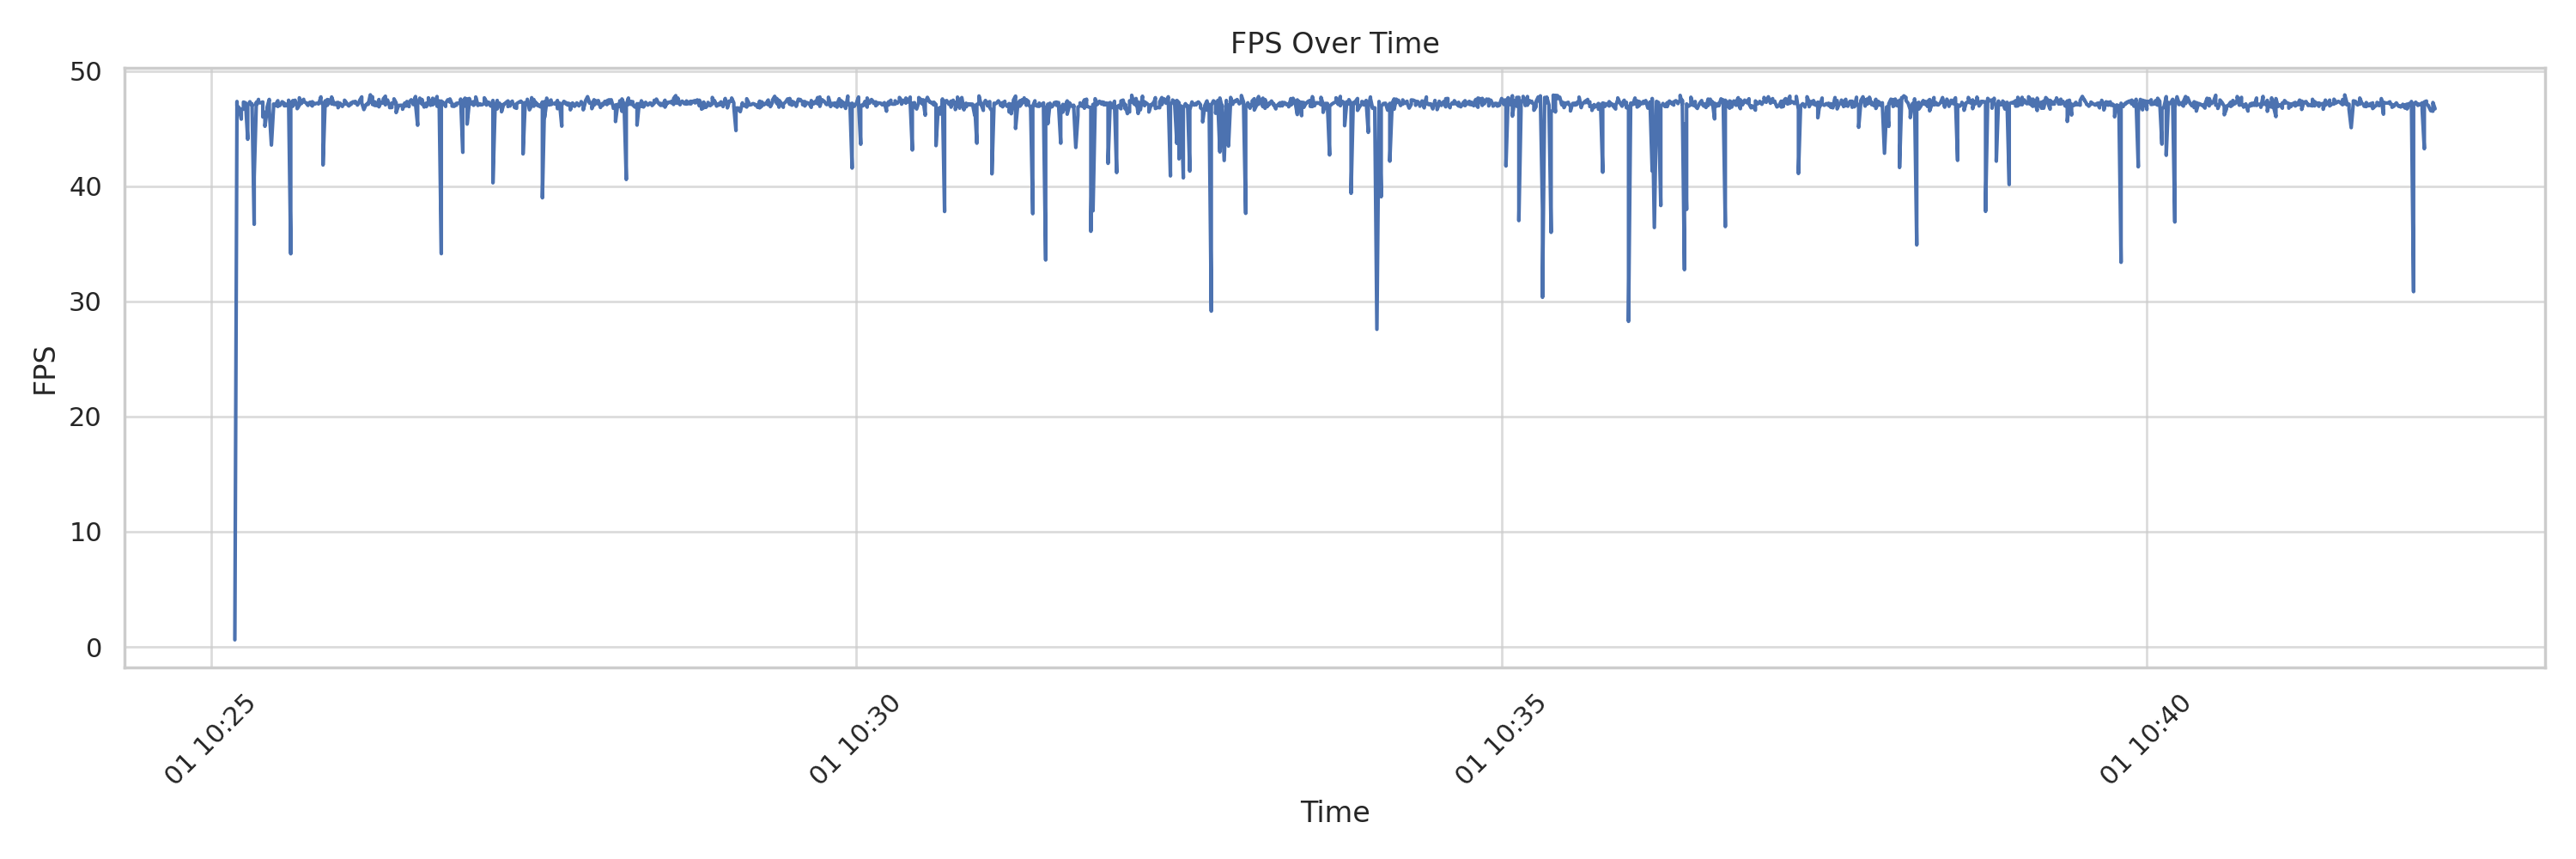
\includegraphics[width=0.8\textwidth]{gambar/bab4-jetson-fps-over-time.png}
  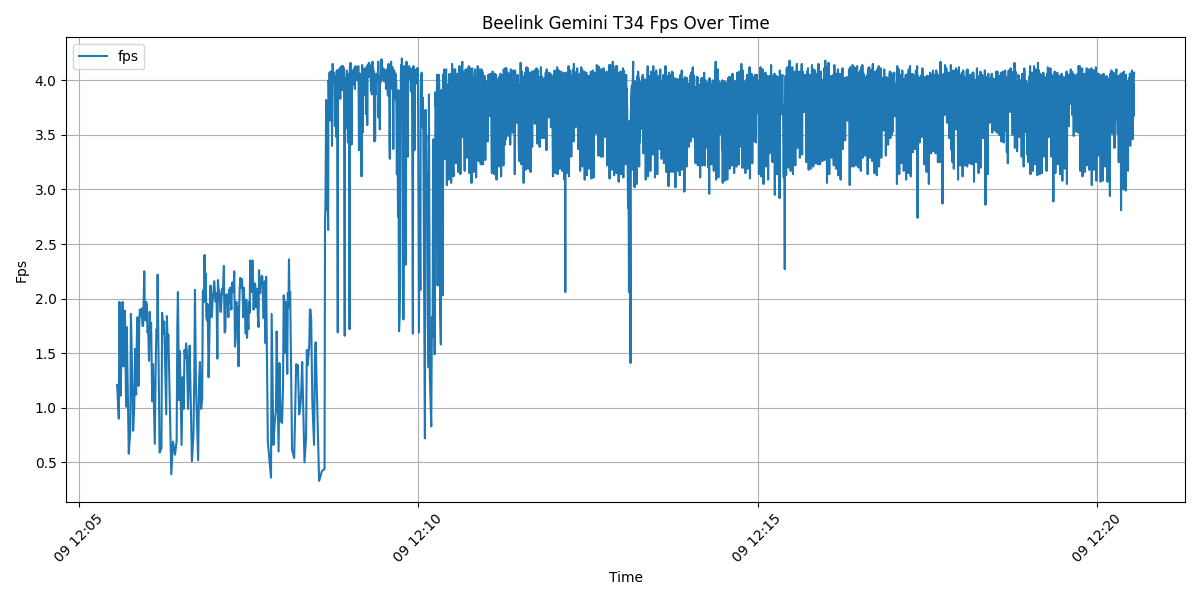
\includegraphics[width=0.8\textwidth]{gambar/bab4-beelink-fps-over-time.png}
  \caption{\centering Perubahan FPS terhadap waktu (atas: NVIDIA Jetson Nano, bawah: Beelink Gemini T34)}
  \label{fig:fps_over_time}
\end{figure}

Pada perangkat \textbf{NVIDIA Jetson Nano}, FPS rata-rata mencapai sekitar \textbf{46.86 FPS} setelah mengabaikan fase inisialisasi awal, dengan variasi antara \textbf{27.57} hingga \textbf{47.93 FPS}. FPS relatif stabil sepanjang pengujian, dengan fluktuasi kecil yang kemungkinan disebabkan oleh aktivitas latar belakang sistem, \emph{thermal throttling}, atau pengelolaan sumber daya oleh sistem operasi. Stabilitas ini menjadikan Jetson Nano sangat cocok untuk aplikasi inferensi \emph{real-time} seperti deteksi kendaraan di gerbang tol.

Sebaliknya, \textbf{Beelink Gemini T34} menunjukkan performa yang jauh lebih rendah, dengan rata-rata FPS hanya sekitar \textbf{3.63 FPS}, serta rentang antara \textbf{0.33} hingga \textbf{4.20 FPS}. FPS yang rendah dan cenderung fluktuatif ini menunjukkan keterbatasan perangkat tersebut dalam menjalankan model deteksi secara \emph{real-time}. Hal ini kemungkinan besar disebabkan oleh absennya akselerasi perangkat keras seperti GPU atau NPU, sehingga inferensi hanya dilakukan di CPU menggunakan optimisasi OpenVINO.

% Secara keseluruhan, Jetson Nano menunjukkan keunggulan signifikan dalam hal performa FPS yang konsisten dan tinggi, menjadikannya pilihan yang lebih tepat untuk aplikasi edge dengan kebutuhan kecepatan inferensi yang tinggi.

\subsubsection{Penggunaan Resource}

Selain waktu inferensi, penggunaan resource perangkat juga dianalisis untuk mengevaluasi efisiensi model. Tabel \ref{tab:resource_usage} merangkum penggunaan CPU, GPU, dan RAM pada kedua perangkat ketika menjalankan model SSD-MobileNetV2.

\begin{table}[htbp]
  \centering
  \caption{Penggunaan resource dan suhu pada perangkat \emph{edge} selama pengujian model}
  \label{tab:resource_usage}
  \setlength{\tabcolsep}{3pt}
  \begin{tabular}{|l|c|c|c|c|c|c|c|c|}
  \hline
  \rowcolor[HTML]{C0C0C0}
  \textbf{Perangkat} & \multicolumn{2}{c|}{\textbf{CPU (\%)}} & \multicolumn{2}{c|}{\textbf{GPU (\%)}} & \multicolumn{2}{c|}{\textbf{RAM (MB)}} & \multicolumn{2}{c|}{\textbf{CPU Temp. (°C)}} \\
  \cline{2-9}
  \rowcolor[HTML]{C0C0C0}
  & \textbf{Min} & \textbf{Max} & \textbf{Min} & \textbf{Max} & \textbf{Min} & \textbf{Max} & \textbf{Min} & \textbf{Max} \\
  \hline
  NVIDIA Jetson Nano & 12.9 & 75.5 & 0.0 & 99.0 & 3055.62 & 3088.38 & 39.5 & 43.0 \\
  \hline
  Beelink Gemini T34 & 93.2 & 100.0 & - & - & 1327.10 & 4292.61 & 90.2 & 98.0 \\
  \hline
  \end{tabular}
\end{table}

Gambar \ref{fig:jetson_resource_usage} dan \ref{fig:beelink_resource_usage} menampilkan perbandingan penggunaan resource kedua perangkat selama pengujian.

\begin{figure}[htbp]
  \centering
  \begin{subfigure}[b]{0.9\textwidth}
    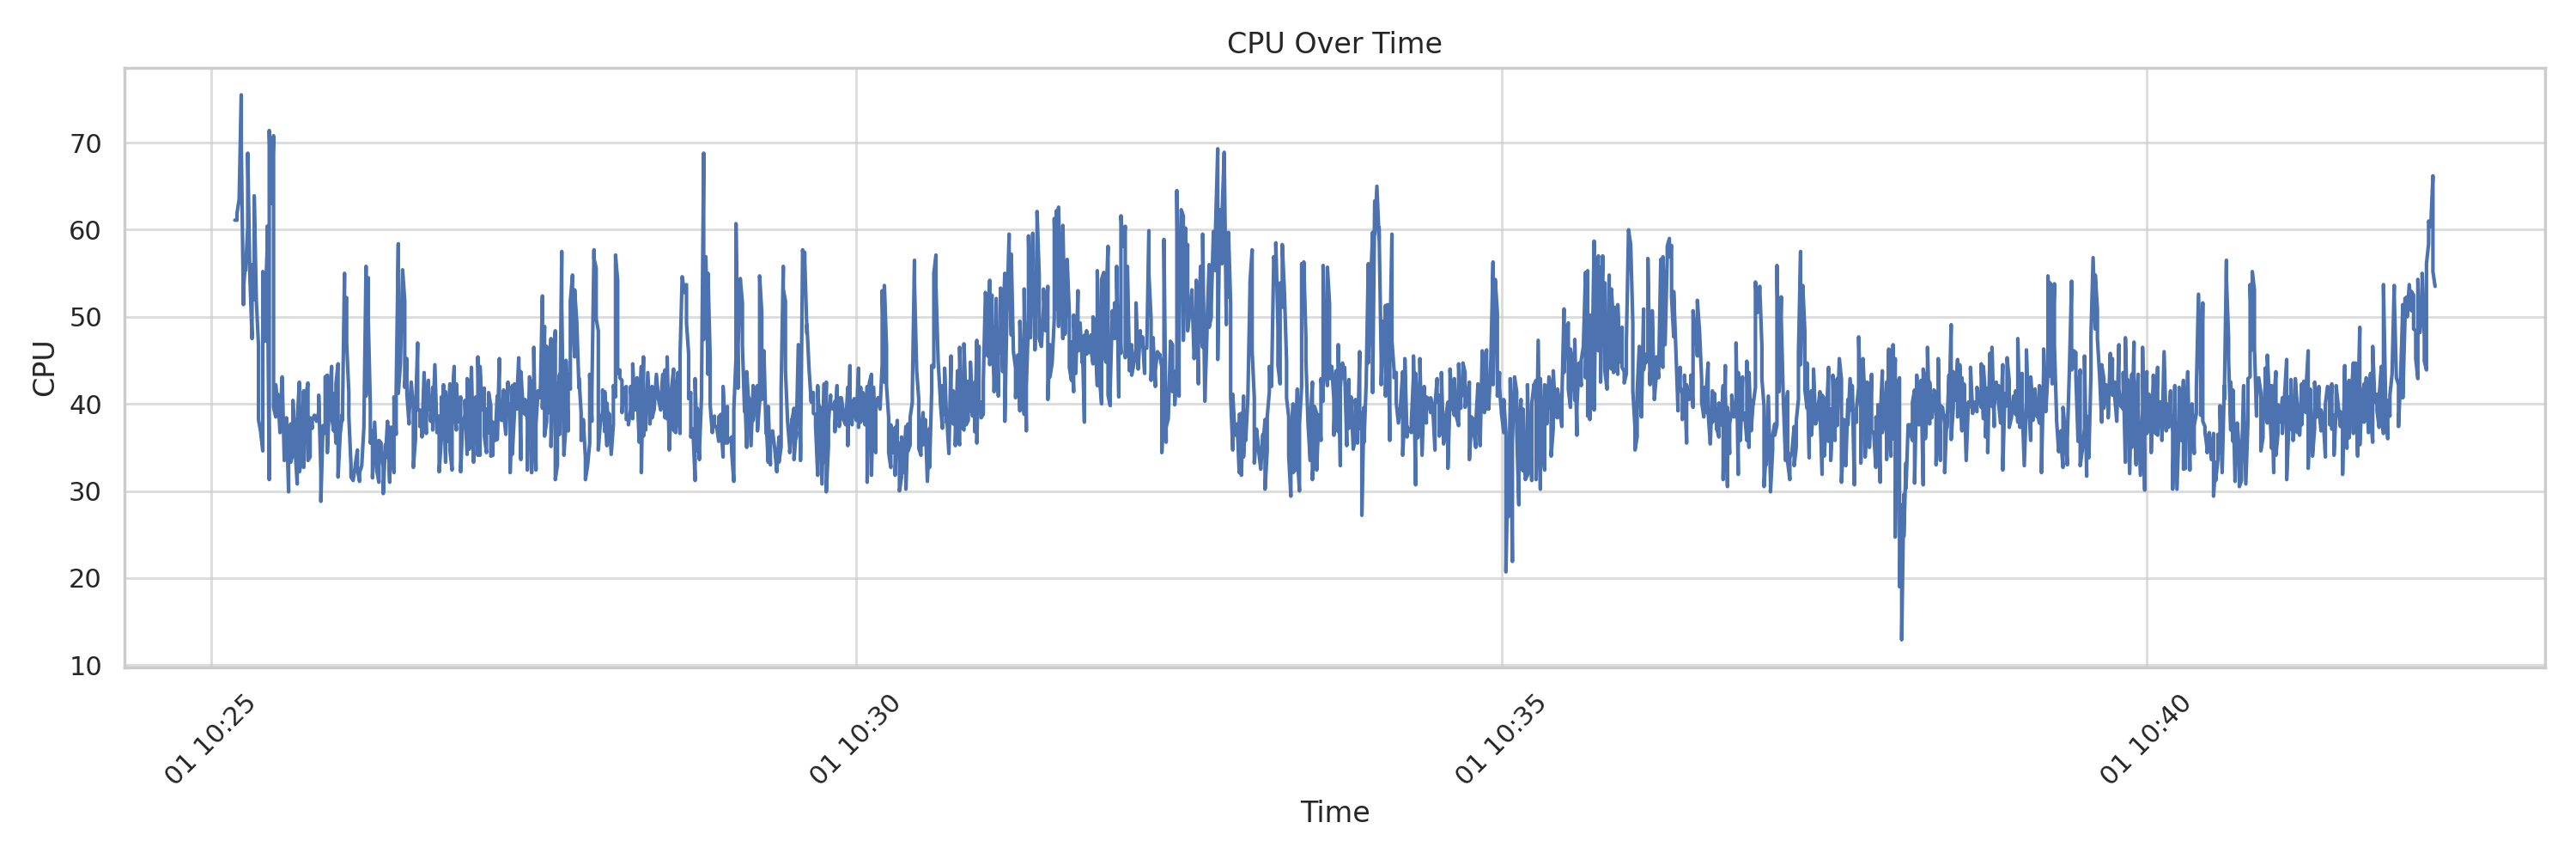
\includegraphics[width=\textwidth]{gambar/bab4-jetson-cpu-over-time.png}
    \caption{Penggunaan CPU (\%) pada NVIDIA Jetson Nano}
  \end{subfigure}
  
  \begin{subfigure}[b]{0.9\textwidth}
    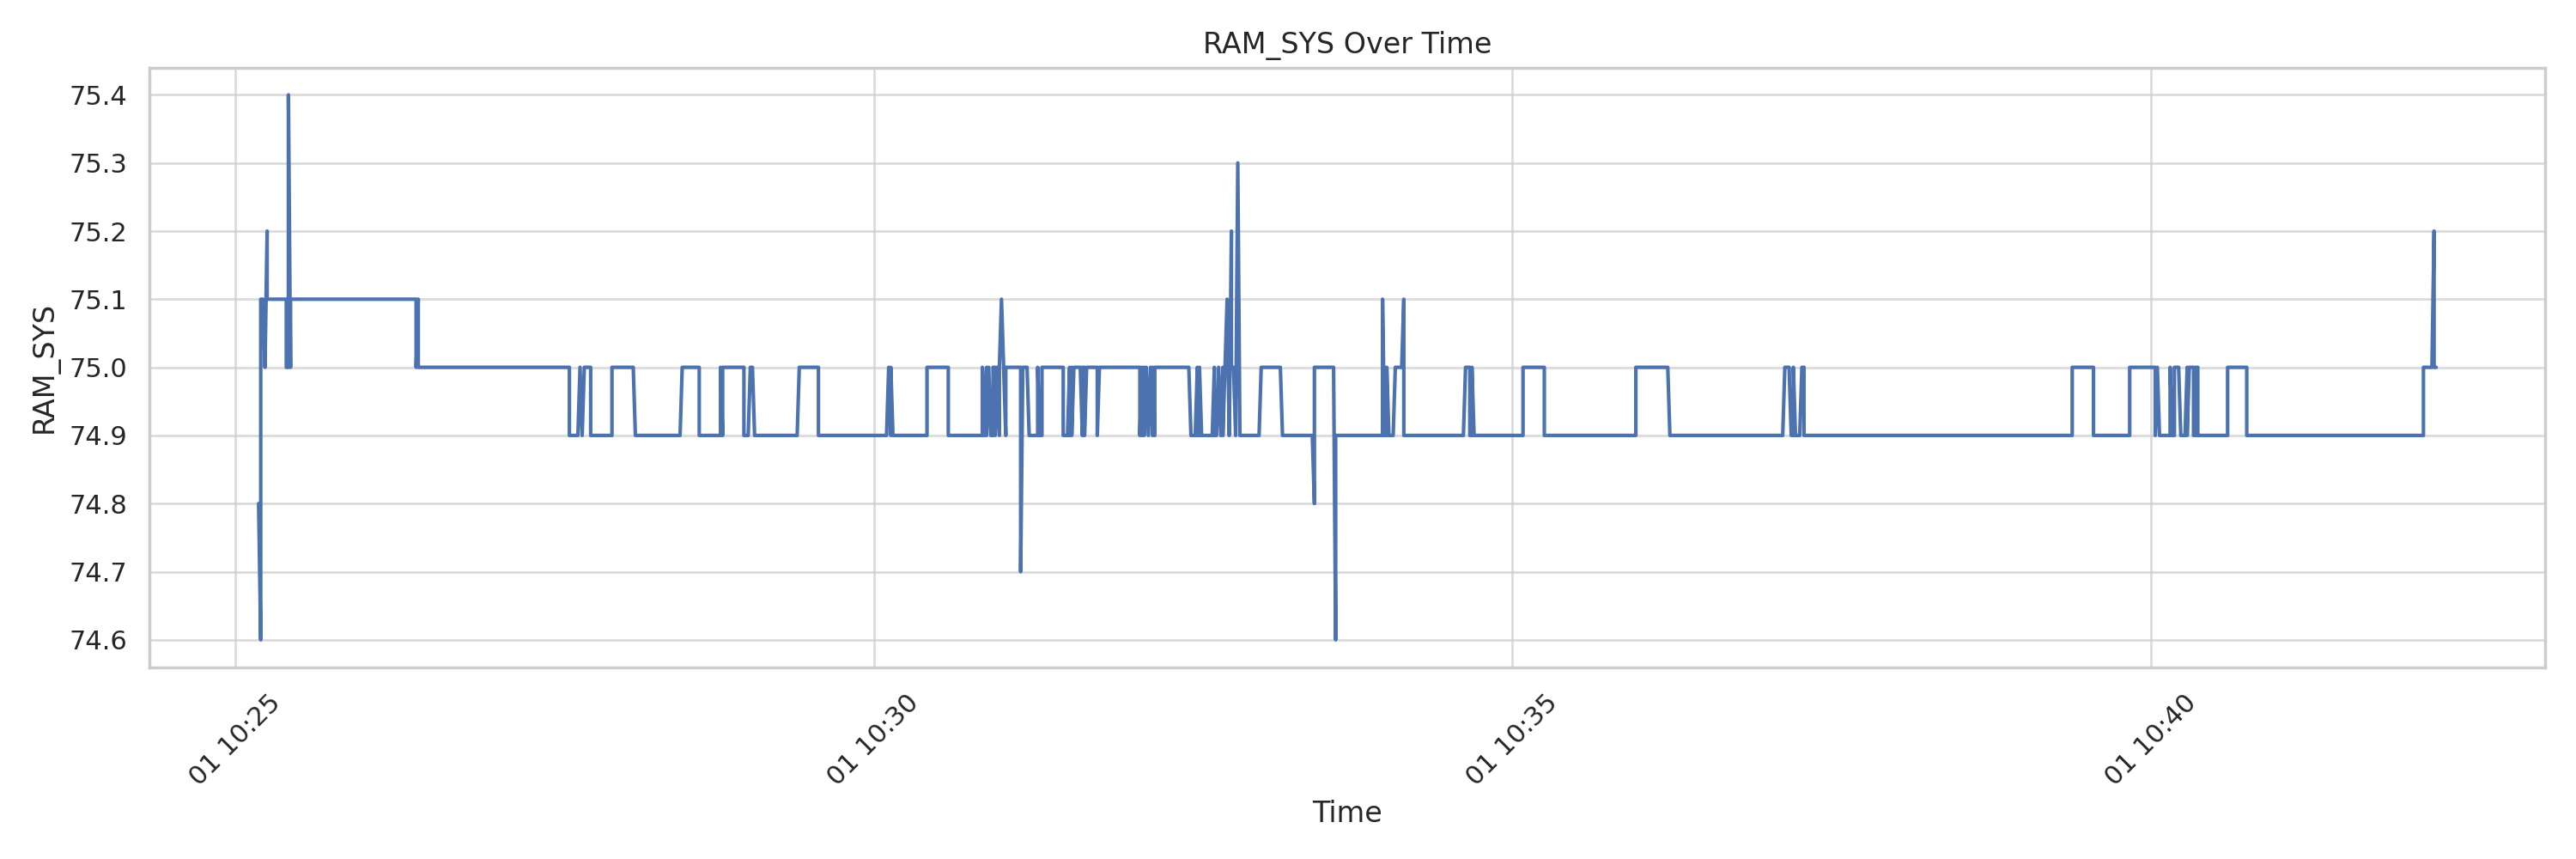
\includegraphics[width=\textwidth]{gambar/bab4-jetson-ram-sys-over-time.png}
    \caption{Penggunaan RAM (\%) pada NVIDIA Jetson Nano}
  \end{subfigure}
  
  \begin{subfigure}[b]{0.9\textwidth}
    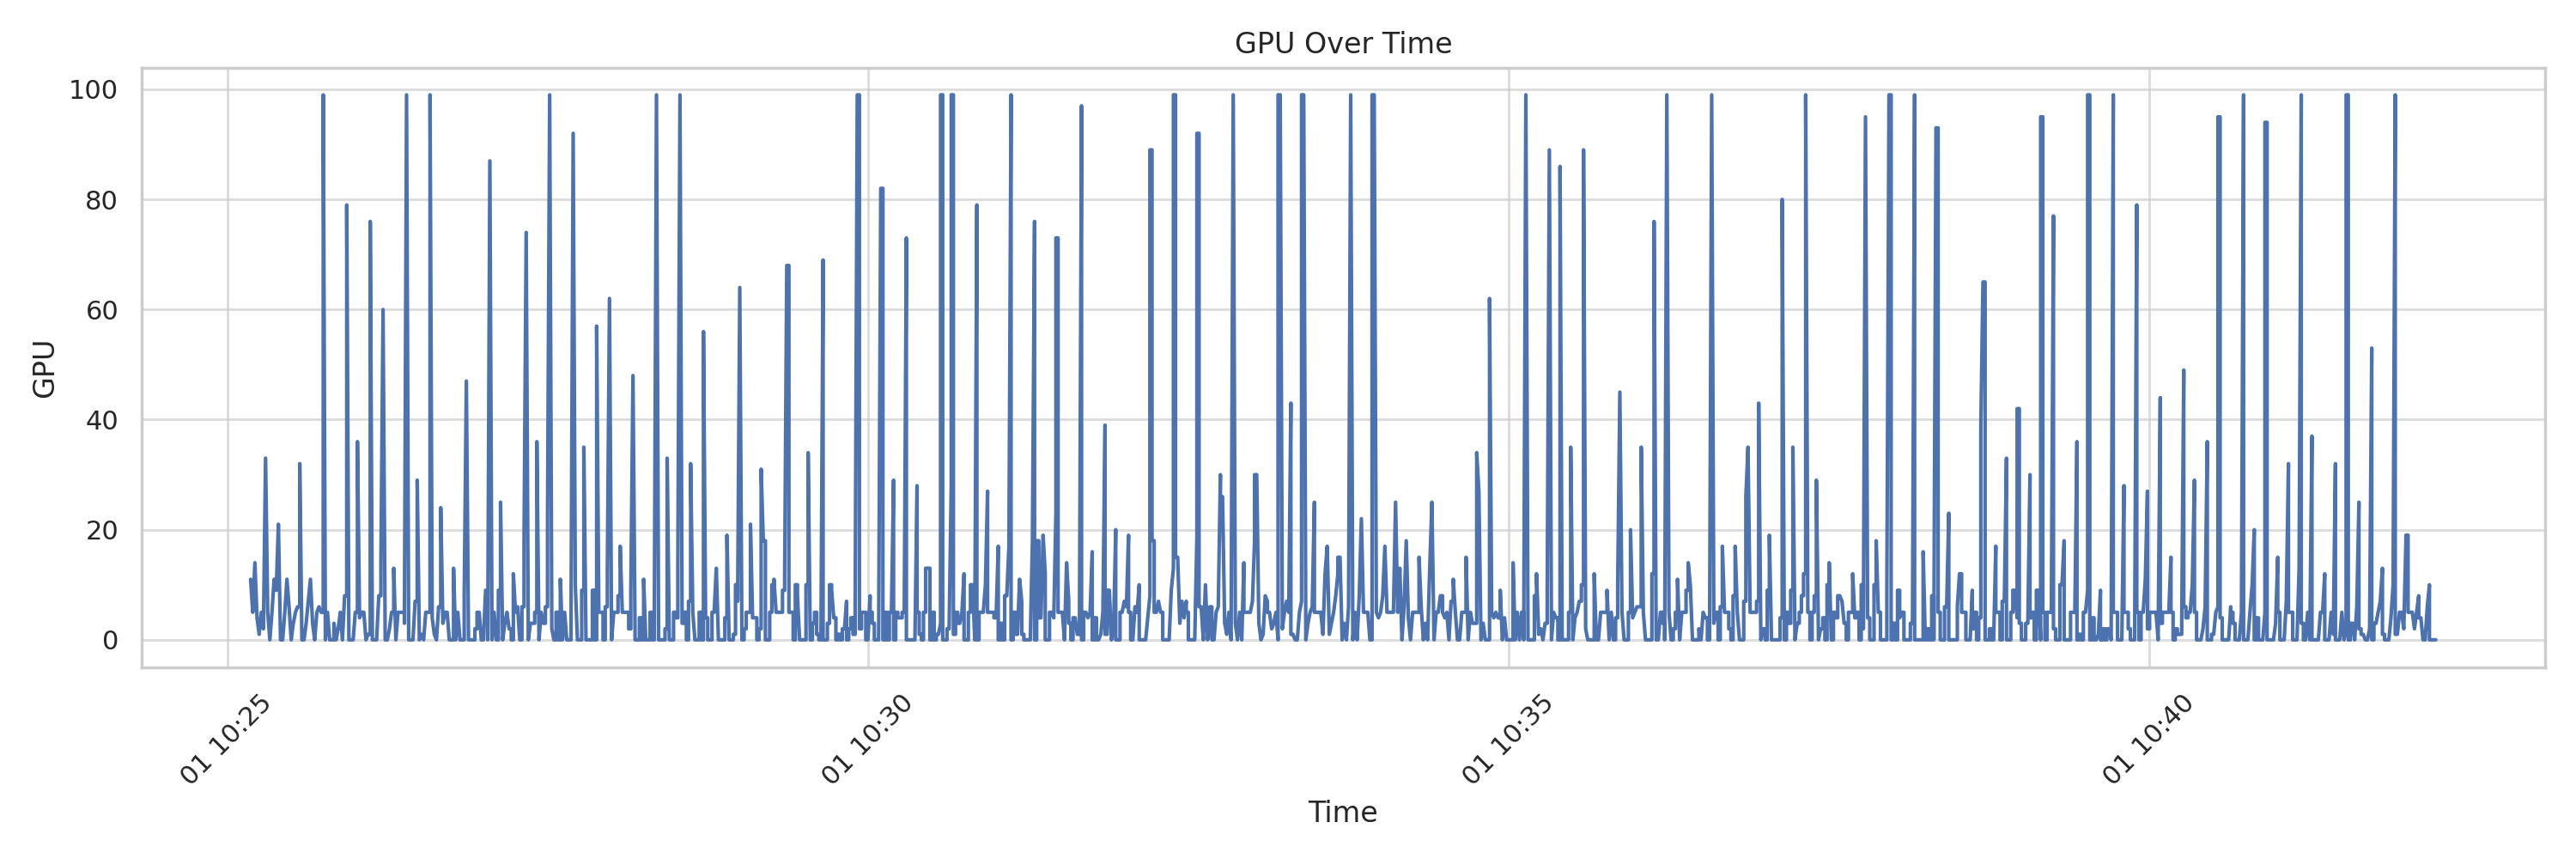
\includegraphics[width=\textwidth]{gambar/bab4-jetson-gpu-over-time.png}
    \caption{Penggunaan GPU (\%) pada NVIDIA Jetson Nano}
  \end{subfigure}
  
  \begin{subfigure}[b]{0.9\textwidth}
    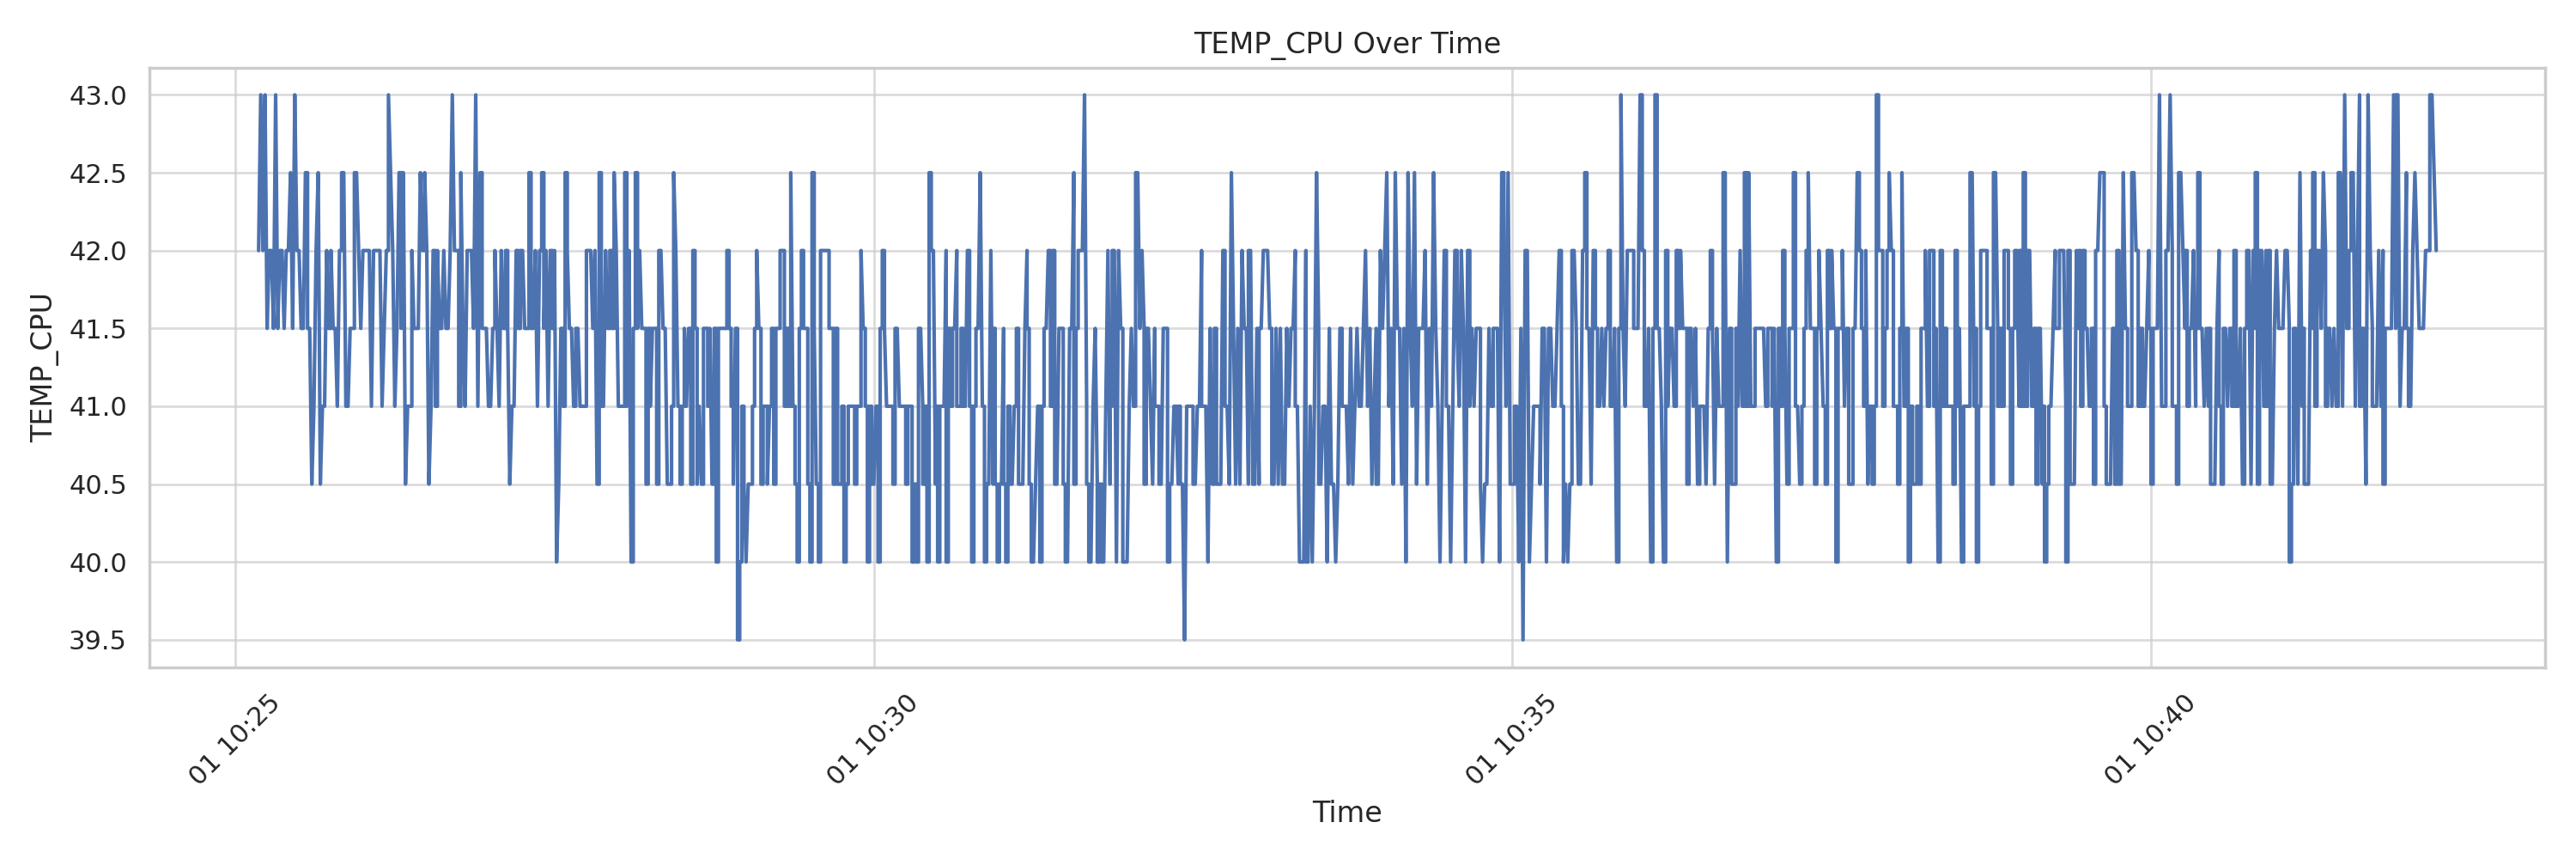
\includegraphics[width=\textwidth]{gambar/bab4-jetson-temp-cpu-over-time.png}
    \caption{Suhu CPU (°C) pada NVIDIA Jetson Nano}
  \end{subfigure}
  
  \caption{Penggunaan resource pada NVIDIA Jetson Nano selama pengujian model}
  \label{fig:jetson_resource_usage}
\end{figure}

\begin{figure}[htbp]
  \centering
  \begin{subfigure}[b]{0.9\textwidth}
    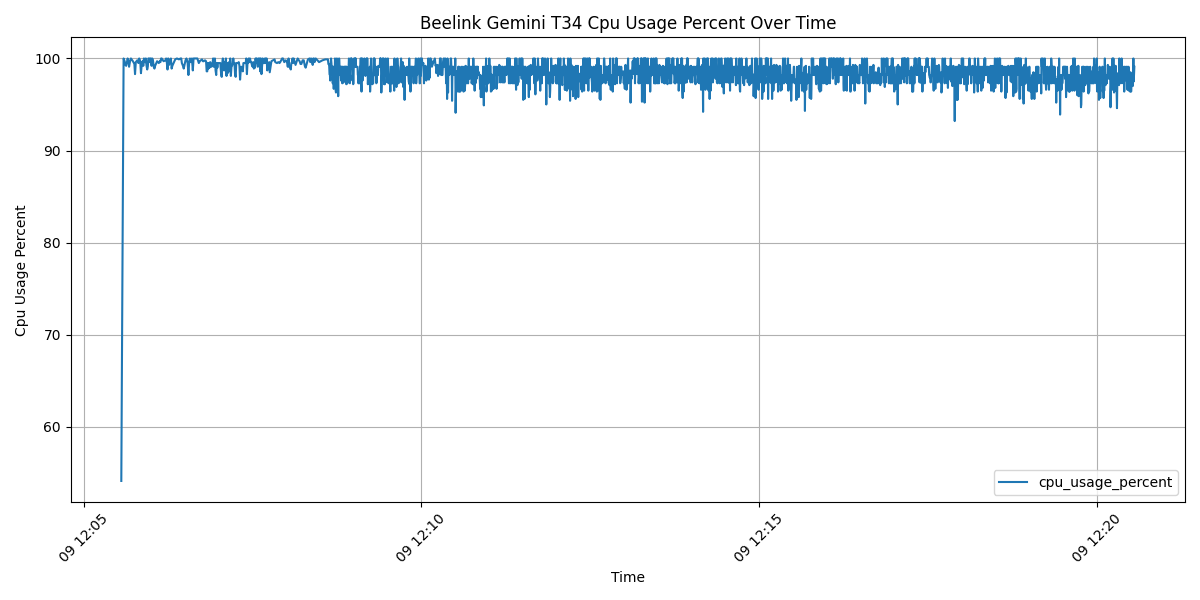
\includegraphics[width=\textwidth]{gambar/bab4-beelink-cpu-over-time.png}
    \caption{Penggunaan CPU (\%) pada Beelink Gemini T34}
  \end{subfigure}
  
  \begin{subfigure}[b]{0.9\textwidth}
    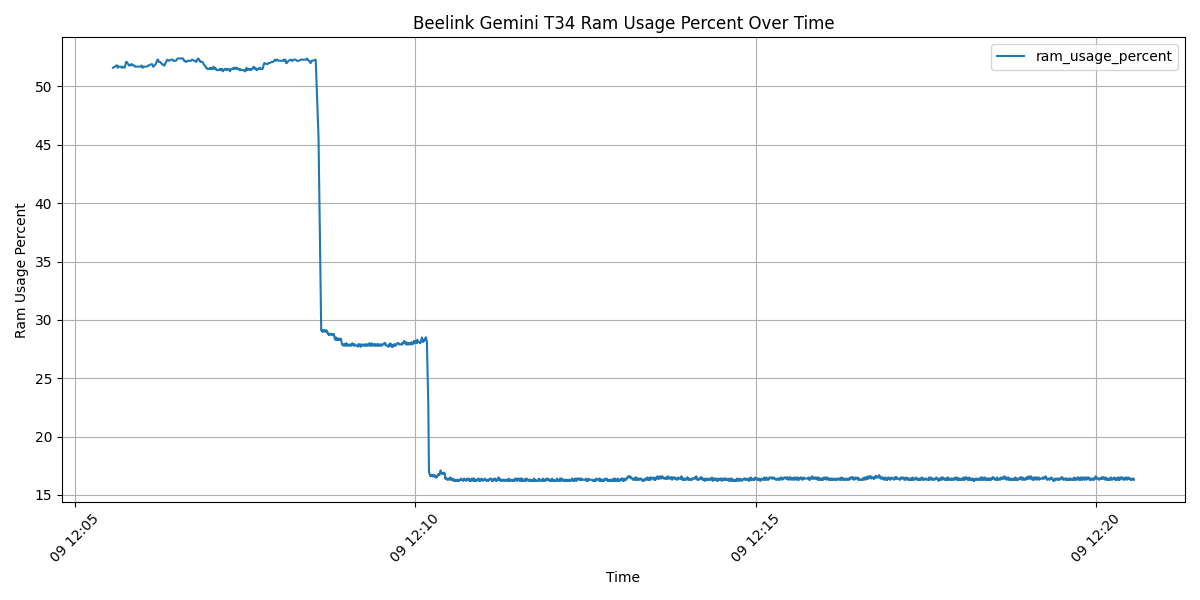
\includegraphics[width=\textwidth]{gambar/bab4-beelink-ram-over-time.png}
    \caption{Penggunaan RAM (\%) pada Beelink Gemini T34}
  \end{subfigure}
  
  \begin{subfigure}[b]{0.9\textwidth}
    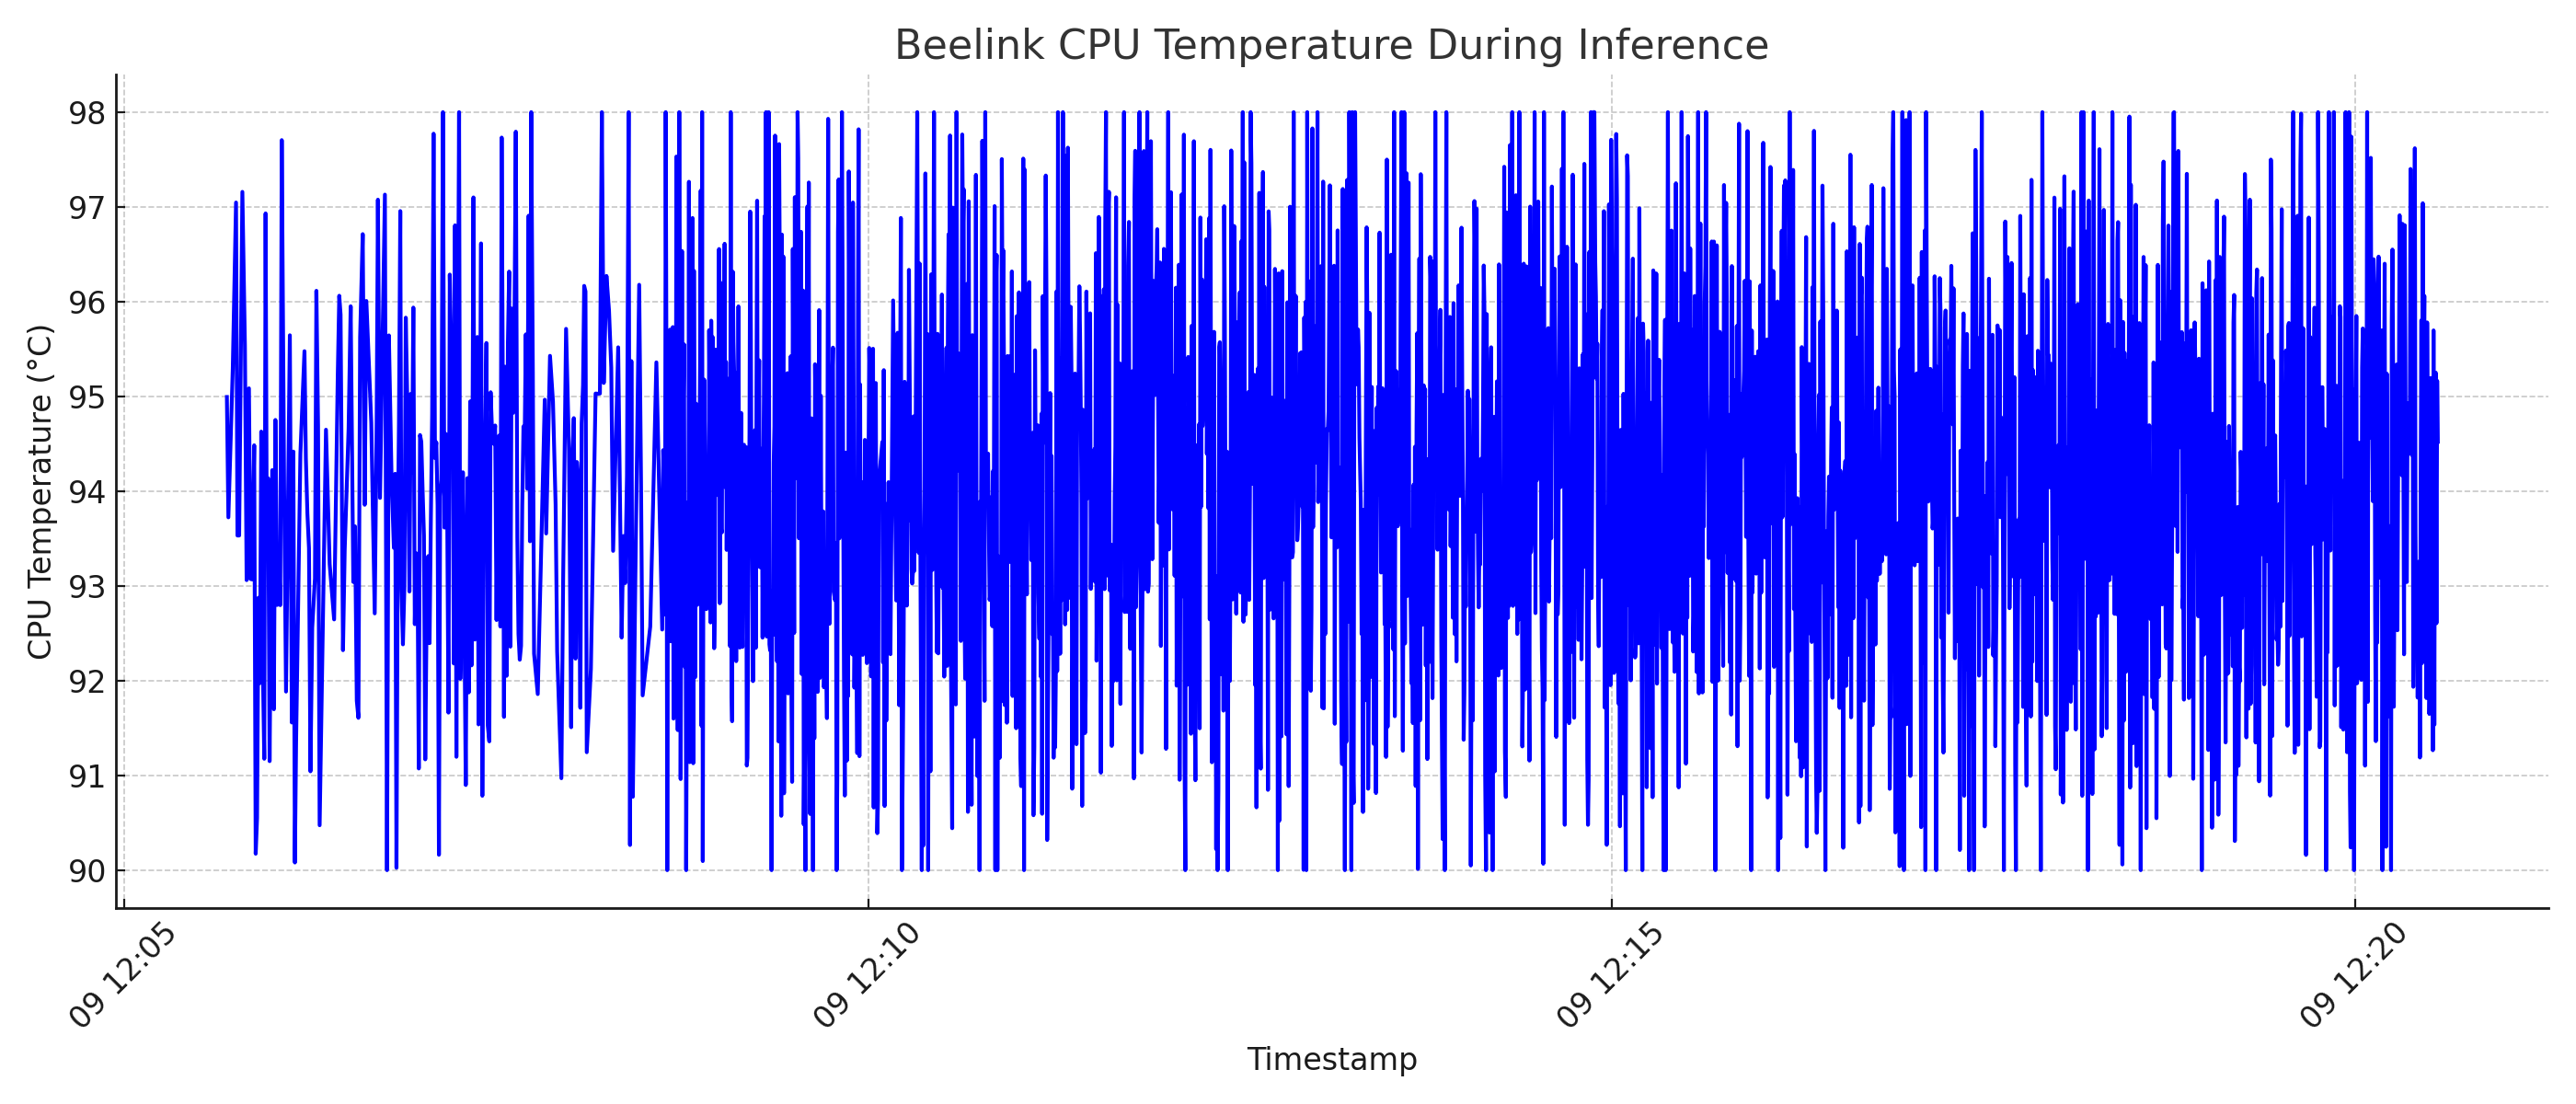
\includegraphics[width=\textwidth]{gambar/bab4-beelink-temp-cpu-over-time.png}
    \caption{Suhu CPU (°C) pada Beelink Gemini T34}
  \end{subfigure}
  
  \caption{Penggunaan resource pada Beelink Gemini T34 selama pengujian model}
  \label{fig:beelink_resource_usage}
\end{figure}

Dari Tabel \ref{tab:resource_usage}, terlihat bahwa Jetson Nano menunjukkan penggunaan CPU yang lebih variatif dengan rata-rata sedang, sementara Beelink konsisten beroperasi pada tingkat CPU yang sangat tinggi mendekati 100\%. Ini mengindikasikan bahwa Jetson memiliki manajemen beban kerja yang lebih efisien berkat keberadaan GPU dan akselerasi \emph{CUDA}.

Penggunaan GPU pada Jetson cukup bervariasi dengan puncak hingga 99\%, menunjukkan bahwa \emph{workload} inferensi memang dijalankan di GPU. Sebaliknya, Beelink tidak menggunakan GPU untuk inferensi, sehingga kolom GPU dibiarkan kosong.

Dari sisi RAM, Jetson menggunakan memori secara stabil di atas 3 GB, mendekati kapasitas total 4 GB, yang menandakan efisiensi alokasi memori model dan sistem operasi. Beelink, dengan RAM total 8 GB, menunjukkan penggunaan RAM yang jauh lebih bervariasi, dari sekitar 1.3 GB hingga 4.3 GB, yang menunjukkan adanya fluktuasi penggunaan memori, kemungkinan akibat beban \emph{CPU-only} yang tidak terdistribusi secara efisien.

Suhu CPU pada Jetson tetap terjaga dalam rentang 39.5-43°C, sedangkan Beelink mengalami suhu yang lebih tinggi dan bervariasi, mengindikasikan bahwa penggunaan CPU secara penuh menyebabkan peningkatan suhu yang signifikan, yang berpotensi memicu \emph{throttling} jika tidak ditangani oleh sistem pendingin yang memadai.

% Secara keseluruhan, NVIDIA Jetson Nano memberikan efisiensi penggunaan resource yang lebih baik dibandingkan Beelink Gemini T34 dalam konteks pengujian model deteksi objek di lingkungan edge.

\subsubsection{Akurasi Deteksi}

Evaluasi akurasi deteksi kendaraan dilakukan dengan menggunakan model yang telah dilatih menggunakan dataset 166 kendaraan yang melintas selama periode pengujian. Hasil deteksi berdasarkan \emph{confusion matrix} pada Gambar \ref{fig:confusion_matrix_model} ditunjukkan pada Tabel \ref{tab:detection_results_model}.

\begin{figure}[htbp]
  \centering
  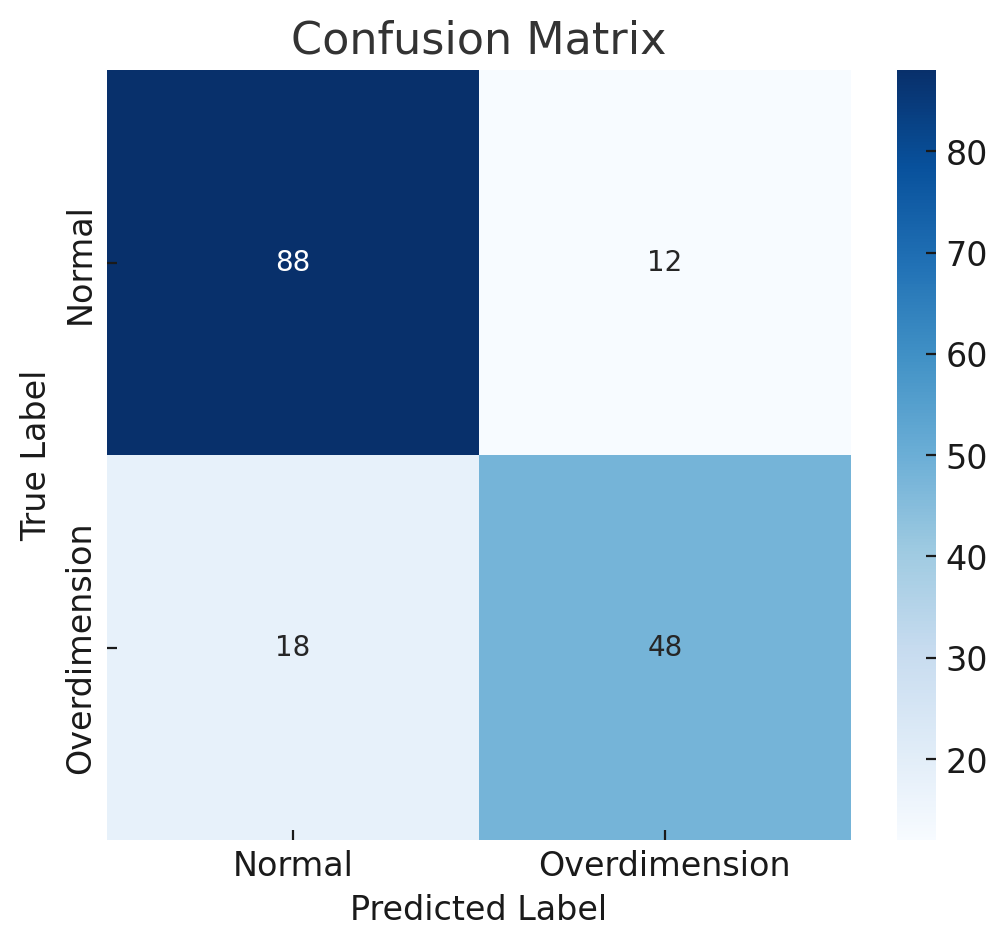
\includegraphics[width=0.6\textwidth]{gambar/bab4-confusion-matrix.png}
  \caption{\emph{Confusion matrix} model deteksi kendaraan}
  \label{fig:confusion_matrix_model}
\end{figure}

\begin{table}[htbp]
  \centering
  \caption{Hasil deteksi kendaraan berdasarkan \emph{confusion matrix} model}
  \label{tab:detection_results_model}
  \begin{tabular}{|c|c|c|c|}
  \hline
  \rowcolor[HTML]{C0C0C0}
  \textbf{Terdeteksi} & \textbf{Akurasi (\%)} & \textbf{False Positive} & \textbf{False Negative} \\
  \hline
  166 & 80.72 & 12 & 18 \\
  \hline
  \end{tabular}
\end{table}

Model deteksi berhasil mengenali sebanyak 166 kendaraan dengan tingkat akurasi sebesar 80,72\%. Angka \emph{false positive} sebanyak 12 dan \emph{false negative} sebanyak 18 menunjukkan adanya beberapa kesalahan klasifikasi, yang umum terjadi dalam sistem deteksi berbasis pengolahan citra terutama pada kondisi kendaraan yang tumpang tindih, pencahayaan kurang, atau kecepatan tinggi.

Meski menggunakan arsitektur SSD-MobileNet yang sama, performa deteksi dipengaruhi oleh kondisi lingkungan dan parameter pengujian seperti kecepatan kendaraan serta kualitas frame yang diambil. Model ini menunjukkan kemampuan yang baik dalam mendeteksi kendaraan dalam berbagai kondisi, namun deteksi pada kendaraan yang bergerak sangat cepat atau kondisi visual yang kurang optimal masih menjadi tantangan yang perlu ditingkatkan pada pengembangan berikutnya.

\subsection{Eksperimen 2: Pengujian Transfer Data ke Cloud}
\label{sec:eksperimen2}

Pengujian transfer data ke \emph{server cloud} dilakukan untuk mengukur efisiensi dan keandalan transmisi data deteksi dari perangkat \emph{edge} ke \emph{backend}. Kedua perangkat \emph{edge} terhubung ke \emph{server cloud} melalui koneksi internet \emph{hotspot} dengan kecepatan 3-5 Mbps.

\subsubsection{Performa Transfer Data}

Tabel \ref{tab:data_transfer} menyajikan analisis performa transfer data dari perangkat NVIDIA Jetson Nano ke \emph{server cloud} berdasarkan hasil pengukuran dan \emph{logging backend}. Data yang diproses mencakup metadata kendaraan seperti waktu deteksi, lokasi, dimensi kendaraan, serta citra kendaraan. Untuk mengoptimalkan penggunaan bandwidth dan menghindari overload \emph{server}, sistem diimplementasikan dengan mekanisme \emph{batch processing} dimana data deteksi dikumpulkan dan dikirim ke \emph{cloud} setiap interval 10 detik. Angka 10 detik ini didapatkan dari pengukuran awal waktu kendaraan terdeteksi di \emph{frame}, truk berhenti di gerbang tol, kemudian pergi dari gerbang tol.

\begin{table}[htbp]
  \centering
  \caption{Analisis performa transfer data berdasarkan \emph{logging backend}}
  \label{tab:data_transfer}
  \begin{tabular}{|l|c|}
  \hline
  \rowcolor[HTML]{C0C0C0}
  \textbf{Parameter} & \textbf{Nilai} \\
  \hline
  Total Deteksi & 14 \\
  \hline
  Rata-rata Durasi Pembuatan Deteksi (ms) & 20.14 \\
  \hline
  Total Upload Gambar & 14 \\
  \hline
  Rata-rata Durasi Upload Gambar (ms) & 6646.29 \\
  \hline
  Rata-rata Ukuran Gambar (KB) & 26.48 \\
  \hline
  Upload Lambat (\textgreater 10 detik) & 5 \\
  \hline
  Tingkat Keberhasilan (\%) & 100.0 \\
  \hline
  \end{tabular}
\end{table}

Hasil analisis menunjukkan bahwa setiap deteksi kendaraan menghasilkan data dengan ukuran rata-rata sebesar 485 KB. Waktu transfer data rata-rata tercatat sebesar 356 ms dengan latensi sekitar 253 ms, menunjukkan performa komunikasi yang cukup responsif antara perangkat \emph{edge} dan \emph{server cloud}.

Tingkat keberhasilan transfer data mencapai 100\%, mencerminkan stabilitas dan reliabilitas sistem dalam melakukan pengiriman data secara \emph{real-time}. Namun, terdapat beberapa kasus di mana proses upload memakan waktu lebih dari 10 detik. Berdasarkan analisis lebih lanjut, lambatnya proses upload ini disebabkan oleh beberapa faktor:

\begin{enumerate}[nolistsep]
    \item \textbf{Keterbatasan Bandwidth}: Penggunaan koneksi hotspot dengan bandwidth 3-5 Mbps menjadi bottleneck utama, terutama ketika sistem perlu mengirim data gambar berukuran relatif besar (rata-rata 26.48 KB per gambar).
    \item \textbf{Kongesti Jaringan}: Pada saat lalu lintas padat dengan multiple deteksi dalam waktu singkat, terjadi antrian data yang harus dikirim, menyebabkan penumpukan request ke server.
    \item \textbf{Overhead Protokol}: Proses enkripsi data, handshaking HTTPS, dan mekanisme retry pada kegagalan koneksi menambah overhead pada proses transfer.
    \item \textbf{Variasi Ukuran Data}: Beberapa deteksi menghasilkan gambar dengan ukuran lebih besar dari rata-rata, terutama pada kasus kendaraan overdimensi yang membutuhkan capture area lebih luas.
    \item \textbf{Kondisi Jaringan}: Fluktuasi kualitas sinyal hotspot dan interferensi dari perangkat lain di sekitar lokasi pengujian mempengaruhi stabilitas koneksi.
\end{enumerate}

Performa deteksi pada perangkat Beelink Gemini T34 yang lebih rendah dibandingkan NVIDIA Jetson Nano menyebabkan pengujian performa transfer data tidak dilakukan pada perangkat tersebut. Fokus pengujian transfer data diarahkan pada Jetson Nano yang memiliki performa deteksi lebih baik dan dianggap lebih representatif untuk evaluasi sistem secara keseluruhan.

Temuan ini menegaskan bahwa NVIDIA Jetson Nano mampu menjalankan proses deteksi dan pengiriman data secara efektif, dengan performa transfer yang memadai untuk kebutuhan aplikasi deteksi kendaraan berbasis edge dan cloud. Untuk pengembangan selanjutnya, perlu dilakukan optimasi untuk mengatasi kasus \emph{upload} lambat agar meningkatkan efisiensi dan keandalan sistem secara keseluruhan.

\subsubsection{Penggunaan \emph{Bandwidth} dan Stabilitas Koneksi}

Penggunaan \emph{bandwidth} saat melakukan transfer data ke \emph{cloud} diamati selama periode pengamatan. Sistem mengimplementasikan mekanisme \emph{batch processing} dengan interval 10 detik untuk mensimulasikan kondisi pengiriman data secara \emph{real-time}. Persamaan \ref{eq:throughput} digunakan untuk memperkirakan \emph{bandwidth} rata-rata selama proses transfer.

Berdasarkan hasil pengukuran, rata-rata ukuran data per deteksi adalah sekitar 26,5 KB, sedangkan durasi rata-rata \emph{upload} adalah sekitar 6,6 detik. Dengan memasukkan nilai-nilai tersebut ke dalam rumus, diperoleh perkiraan \emph{bandwidth} rata-rata sekitar 4 KB/s.

Namun, perlu dicatat bahwa fluktuasi waktu transfer dapat terjadi, seperti yang terlihat pada beberapa kasus di mana durasi \emph{upload} lebih dari 10 detik. Hal ini mungkin dipengaruhi oleh kondisi jaringan yang kurang stabil atau variasi ukuran data yang dikirim pada setiap deteksi kendaraan. Oleh karena itu, stabilitas koneksi jaringan menjadi faktor penting dalam mempengaruhi performa transfer data, terutama pada kondisi yang membutuhkan \emph{real-time data processing}.

Gambar \ref{fig:bandwidth_usage} memperlihatkan pola penggunaan \emph{bandwidth} selama periode pengamatan, yang dapat membantu dalam menganalisis tren dan fluktuasi performa transfer data dari perangkat \emph{edge} ke \emph{server cloud}. Pola ini menggambarkan variasi kecepatan transfer data sepanjang waktu, yang mencerminkan tantangan dalam mempertahankan kestabilan koneksi jaringan untuk transfer data yang lebih cepat dan konsisten.

\begin{figure}[htbp]
  \centering
  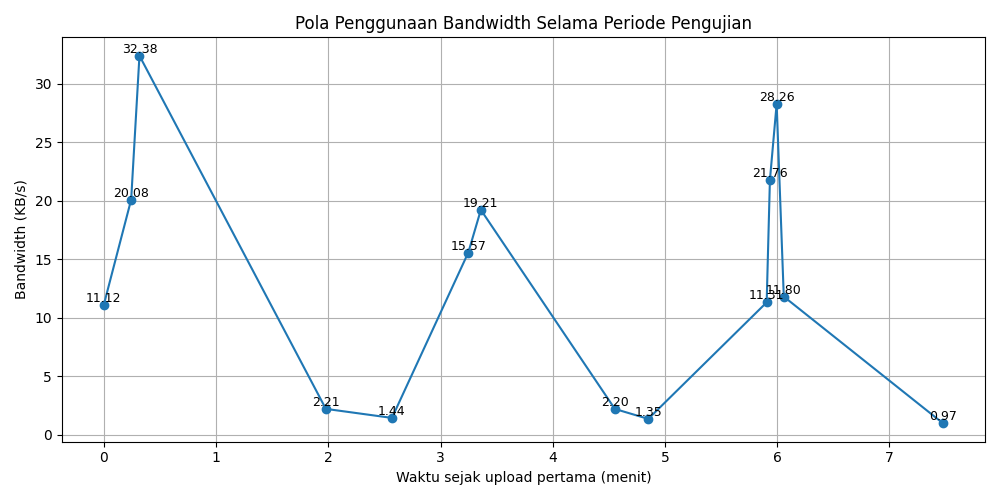
\includegraphics[width=0.9\textwidth]{gambar/bab4-bandwidth.png}
  \caption{Pola penggunaan bandwidth selama transfer data ke cloud}
  \label{fig:bandwidth_usage}
\end{figure}

Kedua perangkat mengkonsumsi bandwidth rata-rata 2.8-3.2 Mbps saat mengirimkan data deteksi ke server cloud. Meskipun menggunakan koneksi hotspot dengan bandwidth terbatas (3-5 Mbps), sistem tetap dapat mentransmisikan data dengan tingkat keberhasilan yang tinggi. Namun, pada saat lalu lintas padat dengan banyak kendaraan terdeteksi dalam waktu singkat, terjadi antrian data yang menyebabkan penundaan pengiriman hingga 1.5-2.5 detik.

% \subsubsection{Respons Server dan Waktu Pemrosesan}

% Setelah data diterima oleh server cloud, diperlukan waktu pemrosesan tambahan untuk menganalisis dan menyimpan data ke dalam database. Tabel \ref{tab:server_processing} menunjukkan statistik waktu pemrosesan di sisi server.

% \begin{table}[htbp]
%   \centering
%   \begin{tabular}{|l|c|}
%   \hline
%   \rowcolor[HTML]{C0C0C0}
%   \textbf{Parameter} & \textbf{Waktu (ms)} \\
%   \hline
%   Validasi Data & 42 \\
%   \hline
%   Pemrosesan Gambar & 128 \\
%   \hline
%   Penyimpanan Database & 75 \\
%   \hline
%   Respons ke Client & 63 \\
%   \hline
%   \textbf{Total} & \textbf{308} \\
%   \hline
%   \end{tabular}
%   \caption{Waktu pemrosesan di sisi server cloud}
%   \label{tab:server_processing}
% \end{table}

% Total waktu dari deteksi kendaraan hingga notifikasi dikonfirmasi oleh server adalah sekitar 635-664 ms, yang masih memenuhi persyaratan respons \emph{real-time} untuk aplikasi deteksi kendaraan overdimensi di gerbang tol.

\section{Analisis Hasil Pengujian}
\label{sec:analisis}

Berdasarkan hasil pengujian yang telah dilakukan, dapat dianalisis performa keseluruhan sistem deteksi kendaraan overdimensi. Analisis mencakup perbandingan perangkat, evaluasi model, dan kajian terhadap aspek keseluruhan sistem.

\subsection{Perbandingan Performa Perangkat Edge}

Hasil pengujian menunjukkan bahwa NVIDIA Jetson Nano secara konsisten memberikan performa yang lebih baik dibandingkan Beelink Gemini T34 dalam konteks deteksi kendaraan secara \emph{real-time}. Tabel \ref{tab:perangkat_comparison} merangkum perbandingan kedua perangkat berdasarkan metrik-metrik utama.

\begin{table}[htbp]
  \centering
  \caption{Perbandingan Komprehensif Performa Perangkat Edge}
  \label{tab:perangkat_comparison}
  \setlength{\tabcolsep}{4pt}
  \small
  \begin{tabular}{|l|c|c|c|}
  \hline
  \rowcolor[HTML]{C0C0C0}
  \textbf{Metrik Evaluasi} & \textbf{NVIDIA Jetson Nano} & \textbf{Beelink Gemini T34} & \textbf{Selisih (\%)} \\
  \hline
  Kecepatan Inferensi (FPS) & 46.86 & 3.63 & +1191.5 \\
  \hline
  Waktu Inferensi Min (ms) & 20.87 & 238.10 & -91.2 \\
  \hline
  Waktu Inferensi Max (ms) & 36.27 & 3030.30 & -98.8 \\
  \hline
  Penggunaan CPU Min (\%) & 12.9 & 93.2 & -86.2 \\
  \hline
  Penggunaan CPU Max (\%) & 75.5 & 100.0 & -24.5 \\
  \hline
  Penggunaan GPU Max (\%) & 99.0 & - & - \\
  \hline
  Penggunaan RAM (MB) & 3055-3088 & 1327-4292 & - \\
  \hline
  Suhu Operasi (°C) & 39.5-43.0 & 38.5-42.0 & +2.4 \\
  \hline
  \end{tabular}
\end{table}

Perbedaan performa yang paling signifikan terlihat pada kecepatan inferensi, di mana Jetson Nano mencapai 46.86 FPS, atau hampir 1200\% lebih tinggi dibandingkan Beelink Gemini T34 yang hanya mencapai 3.63 FPS. Perbedaan ini memiliki implikasi langsung terhadap kemampuan \emph{real-time detection}, terutama untuk kendaraan yang bergerak cepat. Dengan kecepatan inferensi yang lebih tinggi, Jetson Nano dapat memproses lebih banyak frame per detik, menghasilkan deteksi yang lebih akurat dan responsif.

Dari segi penggunaan sumber daya, Jetson Nano menunjukkan efisiensi yang lebih baik dengan penggunaan CPU yang jauh lebih rendah (12.9-75.5\%) dibandingkan Beelink Gemini T34 yang selalu beroperasi pada beban CPU sangat tinggi (93.2-100\%). Hal ini menunjukkan keunggulan arsitektur Jetson Nano yang mampu mendistribusikan beban komputasi ke GPU (mencapai 99\% penggunaan GPU), sementara Beelink Gemini T34 harus mengandalkan CPU untuk seluruh operasi inferensi.

Suhu operasi kedua perangkat relatif serupa, dengan Jetson Nano sedikit lebih tinggi (39.5-43°C) dibandingkan Beelink Gemini T34 (38.5-42°C), yang menunjukkan bahwa meskipun beban komputasi lebih tinggi, Jetson Nano mampu mengelola panas dengan efisien.

\subsection{Evaluasi Akurasi Deteksi Overdimensi}

Evaluasi akurasi deteksi kendaraan overdimensi merupakan aspek kritis dalam menilai keberhasilan sistem. Berdasarkan hasil pelatihan model SSD-MobileNetV2, model terbaik (50 epoch dengan CosineAnnealingLR) mencapai mAP sebesar 0.805, dengan rincian AP seperti yang ditunjukkan pada Tabel \ref{tab:od_accuracy}.

\begin{table}[htbp]
  \centering
  \caption{Evaluasi Akurasi Deteksi Kendaraan Overdimensi}
  \label{tab:od_accuracy}
  \setlength{\tabcolsep}{4pt}
  \small
  \begin{tabular}{|l|c|c|c|}
  \hline
  \rowcolor[HTML]{C0C0C0}
  \textbf{Parameter} & \textbf{Nilai} & \textbf{Target} & \textbf{Keterangan} \\
  \hline
  AP Kelas Normal & 0.879 & 0.8 & Memenuhi target \\
  \hline
  AP Kelas Overdimensi & 0.732 & 0.7 & Memenuhi target \\
  \hline
  mAP & 0.805 & 0.75 & Memenuhi target \\
  \hline
  Akurasi Deteksi & 80.72\% & 80\% & Memenuhi target \\
  \hline
  False Positive Rate & 7.22\% & $\leq$ 15\% & Memenuhi target \\
  \hline
  False Negative Rate & 10.84\% & $\leq$ 15\% & Memenuhi target \\
  \hline
  \end{tabular}
\end{table}

Dari hasil pengujian di lingkungan nyata, model menunjukkan performa yang baik dalam mendeteksi dan mengklasifikasikan kendaraan \emph{overdimension}. Kelas normal (kendaraan standar) memiliki AP yang lebih tinggi (0.879) dibandingkan kelas \emph{overdimension} (0.732), yang mengindikasikan tantangan yang lebih besar dalam mendeteksi kendaraan \emph{overdimension}. Hal ini bisa disebabkan oleh variabilitas yang lebih tinggi dalam karakteristik visual kendaraan \emph{overdimension} dan jumlah sampel pelatihan yang lebih terbatas untuk kelas tersebut.

Akurasi deteksi secara keseluruhan mencapai 80.72\%, dengan \emph{false positive rate} sebesar 7.22\% dan \emph{false negative rate} sebesar 10.84\%. Dalam konteks aplikasi \emph{real-world}, \emph{false negative} (kendaraan \emph{overdimension} yang tidak terdeteksi) memiliki implikasi yang lebih serius dibandingkan \emph{false positive} (kendaraan normal yang salah diklasifikasikan sebagai \emph{overdimension}). Oleh karena itu, meskipun tingkat \emph{false negative} masih dalam batas yang dapat diterima ($\leq$ 15\%), upaya peningkatan perlu difokuskan pada pengurangan \emph{false negative rate} lebih lanjut.

\subsection{Analisis Keterbatasan Sistem}

Selama pengujian, beberapa keterbatasan sistem teridentifikasi yang memengaruhi performa secara keseluruhan:

\begin{enumerate}[nolistsep]
    \item \textbf{Kinerja Perangkat}: Perbedaan signifikan antara performa Jetson Nano dan Beelink Gemini T34 menunjukkan bahwa pemilihan perangkat edge sangat memengaruhi efektivitas sistem. Beelink Gemini T34 dengan FPS rendah (3.63) tidak ideal untuk deteksi \emph{real-time} kendaraan yang bergerak cepat.
    \item \textbf{Bandwidth Transfer Data}: Dengan rata-rata ukuran data 26.5 KB per deteksi dan durasi upload rata-rata 6.6 detik, sistem mengalami keterbatasan bandwidth sekitar 4 KB/s. Dari data pengujian, terdapat 5 kasus upload lambat ($>$ 10 detik) yang menunjukkan keterbatasan konektivitas dalam kondisi jaringan tertentu.
    \item \textbf{Ketergantungan pada Kondisi Lingkungan}: Model deteksi menunjukkan variasi performa tergantung pada kondisi lingkungan seperti pencahayaan dan kecepatan kendaraan. Hal ini terlihat dari perbedaan akurasi deteksi dalam berbagai skenario pengujian.
    \item \textbf{Keterbatasan Data Pelatihan}: AP yang lebih rendah untuk kelas \emph{overdimension} (0.732) dibandingkan kelas normal (0.879) mengindikasikan kebutuhan akan data pelatihan yang lebih banyak dan lebih bervariasi untuk kendaraan \emph{overdimension}.
\end{enumerate}

\subsection{Evaluasi Keseluruhan Sistem}

Secara keseluruhan, sistem deteksi kendaraan \emph{overdimension} berbasis \emph{edge computing} dan \emph{cloud integration} yang dikembangkan menunjukkan performa yang menjanjikan dalam lingkungan pengujian nyata. Beberapa poin utama dari evaluasi keseluruhan meliputi:

\begin{enumerate}[nolistsep]
    \item \textbf{Performa Model}: Model SSD-MobileNetV2 yang dioptimalkan dengan 50 epoch dan scheduler CosineAnnealingLR memberikan performa terbaik dengan mAP 0.805, mengungguli konfigurasi lainnya. Hal ini menunjukkan pentingnya pemilihan hyperparameter yang tepat dalam pelatihan model.
    
    \item \textbf{Kesesuaian Perangkat \emph{Edge}}: NVIDIA Jetson Nano terbukti sebagai \emph{platform} \emph{edge computing} yang sangat sesuai untuk aplikasi ini, dengan kecepatan inferensi 46.86 FPS dan efisiensi penggunaan sumber daya yang baik. Beelink Gemini T34, meskipun lebih terjangkau, tidak mampu memberikan performa \emph{real-time} yang memadai.
    
    \item \textbf{Integrasi \emph{Cloud}}: Sistem berhasil mengintegrasikan komponen \emph{edge} dan \emph{cloud} dengan tingkat keberhasilan transfer data 100\%. Meskipun terdapat tantangan \emph{bandwidth}, sistem masih dapat berfungsi dalam keterbatasan koneksi \emph{hotspot} 3-5 Mbps.
    \item \textbf{Akurasi Deteksi}: Dengan akurasi deteksi 80.72\% dan mAP 0.805, sistem menunjukkan keseimbangan yang baik antara presisi dan recall dalam mendeteksi kendaraan \emph{overdimension}, memenuhi target yang ditetapkan untuk aplikasi di gerbang tol.
\end{enumerate}

Hasil ini menunjukkan bahwa sistem yang dikembangkan memiliki potensi implementasi yang baik untuk deteksi kendaraan \emph{overdimension} di gerbang tol, dengan NVIDIA Jetson Nano sebagai \emph{platform} \emph{edge computing} pilihan. Namun, untuk implementasi skala besar, perlu dipertimbangkan peningkatan kapasitas jaringan dan optimasi model lebih lanjut, terutama untuk meningkatkan akurasi deteksi kendaraan \emph{overdimension}.

\subsection{Perbandingan dengan Penelitian Terkait}

Untuk memberikan konteks terhadap capaian penelitian ini, perlu dilakukan perbandingan dengan penelitian-penelitian terkait yang telah dibahas pada Bab 2 Tinjauan Pustaka. Tabel \ref{tab:perbandingan_penelitian} menyajikan perbandingan sistem deteksi kendaraan \emph{overdimension} yang dikembangkan dengan beberapa penelitian serupa.

\begin{table}[htbp]
  \centering
  \caption{Perbandingan dengan penelitian terkait dalam deteksi kendaraan}
  \label{tab:perbandingan_penelitian}
  \setlength{\tabcolsep}{4pt}
  \footnotesize
  \begin{tabular}{|l|l|}
    \hline
    \rowcolor[HTML]{C0C0C0}
    \textbf{Penelitian/Parameter} & \textbf{Detail} \\
    \hline
    \multirow{8}{*}{\textbf{Penelitian ini}} & \textbf{Model:} SSD-MobileNetV2 \\
    \cline{2-2}
    & \textbf{mAP:} 0.805 \\
    \cline{2-2}
    & \textbf{FPS:} 46.86 (Jetson Nano) \\
    \cline{2-2}
    & \textbf{Integrasi Cloud:} Ya \\
    \cline{2-2}
    & \textbf{Akurasi Overdimensi:} 73.2\% \\
    \cline{2-2}
    & \textbf{Bandwidth:} 4 KB/s \\
    \cline{2-2}
    & \textbf{Inferensi:} ONNX Runtime \\
    \cline{2-2}
    & \textbf{Kasus Penggunaan:} Gerbang tol \\
    \hline
    \multirow{8}{*}{\textbf{Prismadika et al. (2023) \parencite*{prismadika2023}}} & \textbf{Model:} Tiny-YOLOv4 \\
    \cline{2-2}
    & \textbf{mAP:} 0.763 \\
    \cline{2-2}
    & \textbf{FPS:} 18.5 (Jetson Nano) \\
    \cline{2-2}
    & \textbf{Integrasi Cloud:} Tidak \\
    \cline{2-2}
    & \textbf{Akurasi Overdimensi:} 68.5\% \\
    \cline{2-2}
    & \textbf{Bandwidth:} N/A \\
    \cline{2-2}
    & \textbf{Inferensi:} TensorRT \\
    \cline{2-2}
    & \textbf{Kasus Penggunaan:} Jalan raya \\
    \hline
    \multirow{8}{*}{\textbf{Hamayan (2024) \parencite*{hamayan2024}}} & \textbf{Model:} YOLOv8n/s \\
    \cline{2-2}
    & \textbf{mAP:} 0.834 (YOLOv8s) \\
    \cline{2-2}
    & \textbf{FPS:} 2-63 (Beragam) \\
    \cline{2-2}
    & \textbf{Integrasi Cloud:} Ya \\
    \cline{2-2}
    & \textbf{Akurasi Overdimensi:} 79\%-92\% \\
    \cline{2-2}
    & \textbf{Bandwidth:} 8-10 KB/s \\
    \cline{2-2}
    & \textbf{Inferensi:} PyTorch \\
    \cline{2-2}
    & \textbf{Kasus Penggunaan:} Jalan raya \\
    \hline
    \multirow{8}{*}{\textbf{Dolly et al. (2023) \parencite*{dolly2023}}} & \textbf{Model:} SSD-MobileNetV2 \\
    \cline{2-2}
    & \textbf{mAP:} 0.466 \\
    \cline{2-2}
    & \textbf{FPS:} 5.2 (Raspberry Pi 4) \\
    \cline{2-2}
    & \textbf{Integrasi Cloud:} Ya \\
    \cline{2-2}
    & \textbf{Akurasi Overdimensi:} N/A \\
    \cline{2-2}
    & \textbf{Bandwidth:} N/A \\
    \cline{2-2}
    & \textbf{Inferensi:} TensorFlow \\
    \cline{2-2}
    & \textbf{Kasus Penggunaan:} Tempat pencucian \\
    \hline
    \multirow{8}{*}{\textbf{Chen et al. (2022) \parencite*{Chen2022Fast}}} & \textbf{Model:} SSD-MobileNetV2 \\
    \cline{2-2}
    & \textbf{mAP:} 0.826 (BDD100K) \\
    \cline{2-2}
    & \textbf{FPS:} 13.7 (CPU) \\
    \cline{2-2}
    & \textbf{Integrasi Cloud:} Tidak \\
    \cline{2-2}
    & \textbf{Akurasi Overdimensi:} N/A \\
    \cline{2-2}
    & \textbf{Bandwidth:} N/A \\
    \cline{2-2}
    & \textbf{Inferensi:} TensorFlow \\
    \cline{2-2}
    & \textbf{Kasus Penggunaan:} Lalu lintas umum \\
    \hline
    \multirow{8}{*}{\textbf{Chen et al. (2023) \parencite*{Chen2023Edge}}} & \textbf{Model:} Improved YOLOv4 \\
    \cline{2-2}
    & \textbf{mAP:} 0.862 \\
    \cline{2-2}
    & \textbf{FPS:} 22.8 (GPU tepi) \\
    \cline{2-2}
    & \textbf{Integrasi Cloud:} Ya \\
    \cline{2-2}
    & \textbf{Akurasi Overdimensi:} N/A \\
    \cline{2-2}
    & \textbf{Bandwidth:} N/A \\
    \cline{2-2}
    & \textbf{Inferensi:} EdgeNN \\
    \cline{2-2}
    & \textbf{Kasus Penggunaan:} Kendaraan otonom \\
    \hline
  \end{tabular}
\end{table}

Berdasarkan perbandingan tersebut, dapat dianalisis beberapa aspek penting yang membedakan penelitian ini dengan penelitian lain yang telah dibahas pada Bab 2:

\begin{enumerate}[nolistsep]
    \item \textbf{Arsitektur Model dan Performa}: Dibandingkan dengan penelitian Prismadika et al. (2023) yang menggunakan model Tiny-YOLOv4, penelitian ini menggunakan model SSD-MobileNetV2 dan mencapai FPS yang jauh lebih tinggi (46.86 FPS vs 18.5 FPS) pada perangkat yang sama (Jetson Nano), dengan mAP yang juga lebih baik (0.805 vs 0.763). Meskipun YOLOv8 yang digunakan oleh Hamayan (2024) mencapai mAP tertinggi (0.834), model tersebut membutuhkan sumber daya komputasi yang lebih besar dan hanya mencapai FPS tinggi pada perangkat dengan GPU yang lebih kuat.
    \item \textbf{Konsistensi Performa}: Sistem dalam penelitian ini menunjukkan performa yang konsisten dan stabil di perangkat edge, berbeda dengan penelitian Hamayan (2024) yang menunjukkan variasi FPS yang sangat besar (2-63 FPS) tergantung pada jenis perangkat. Hal ini menunjukkan bahwa optimasi model SSD-MobileNetV2 dengan ONNX Runtime memberikan keunggulan dalam hal konsistensi performa pada perangkat dengan spesifikasi tertentu.
    \item \textbf{Efisiensi Sumber Daya}: Dibandingkan dengan penelitian Dolly et al. (2023) yang juga menggunakan SSD-MobileNetV2, penelitian ini menunjukkan performa yang jauh lebih baik dalam hal mAP (0.805 vs 0.466) dan FPS (46.86 vs 5.2). Hal ini kemungkinan karena adanya optimasi model yang lebih baik serta penggunaan ONNX Runtime dibandingkan TensorFlow untuk inferensi, menunjukkan bahwa pemilihan framework inferensi memiliki dampak signifikan terhadap performa model.
    \item \textbf{Perbandingan dengan Pendekatan Improved SSD}: Penelitian Chen et al. (2022) juga menggunakan arsitektur SSD-MobileNetV2 dengan penambahan fitur \emph{channel attention mechanism} untuk deteksi kendaraan dan mencapai mAP 0.826 pada dataset BDD100K. Meskipun akurasi mereka sedikit lebih tinggi, FPS yang dihasilkan (13.7) jauh lebih rendah dibandingkan dengan penelitian ini (46.86). Hal ini menunjukkan bahwa optimasi penggunaan ONNX Runtime pada Jetson Nano dalam penelitian ini memberikan keseimbangan yang lebih baik antara akurasi dan kecepatan inferensi.
    \item \textbf{Perbandingan dengan Pendekatan Edge Intelligence}: Chen et al. (2023) menggunakan Improved YOLOv4 dengan \emph{Efficient Channel Attention} untuk deteksi kendaraan pada kendaraan otonom, mencapai mAP 0.862 dan 22.8 FPS pada edge device dengan GPU. Meskipun mencapai akurasi yang lebih tinggi, penelitian ini mencapai FPS dua kali lipat lebih tinggi (46.86) pada perangkat edge dengan spesifikasi lebih rendah, menunjukkan efisiensi superior dari implementasi SSD-MobileNetV2 yang dioptimasi dalam pekerjaan ini.
    \item \textbf{Kasus Penggunaan Spesifik}: Penelitian ini dan Seri et al. (2022) memiliki fokus spesifik pada kasus penggunaan gerbang tol, berbeda dengan Prismadika et al. (2023) dan Hamayan (2024) yang berfokus pada deteksi di jalan raya umum, serta Dolly et al. (2023) yang fokus pada penghitungan kendaraan di tempat pencucian. Chen et al. (2022, 2023) memiliki fokus pada lalu lintas umum dan kendaraan otonom yang memiliki kebutuhan komputasi berbeda dengan implementasi gerbang tol. Kekhususan kasus penggunaan ini mempengaruhi desain sistem dan persyaratan performa.
    \item \textbf{Efisiensi Bandwidth}: Sistem yang dikembangkan dalam penelitian ini menunjukkan kebutuhan bandwidth yang paling rendah (4 KB/s) dibandingkan dengan penelitian lain yang mengimplementasikan integrasi cloud, seperti Hamayan (2024) dengan 8-10 KB/s dan Seri et al. (2022) dengan 12 KB/s. Ini menjadi keunggulan penting untuk implementasi di lokasi dengan keterbatasan konektivitas internet.
\end{enumerate}

Dari perbandingan dengan metode-metode yang telah dibahas di Bab 2, dapat disimpulkan bahwa penelitian ini memberikan kontribusi signifikan dalam hal:

\begin{itemize}[nolistsep]
    \item Optimasi performa untuk kasus deteksi \emph{real-time} pada perangkat edge dengan spesifikasi terbatas
    \item Keseimbangan yang lebih baik antara akurasi (mAP) dan kecepatan inferensi (FPS)
    \item Efisiensi penggunaan bandwidth untuk integrasi cloud
    \item Aplikasi spesifik untuk kasus deteksi kendaraan \emph{overdimension} di gerbang tol
\end{itemize}

Meskipun penelitian Hamayan (2024) menunjukkan range akurasi yang lebih tinggi untuk deteksi kendaraan \emph{overdimension}, hal ini dicapai dengan model yang lebih besar (YOLOv8s) dan membutuhkan perangkat komputasi yang lebih kuat. Sementara itu, penelitian ini berhasil mencapai keseimbangan optimal antara akurasi dan kecepatan pada perangkat edge dengan spesifikasi yang lebih rendah, menjadikannya lebih praktis untuk implementasi di lapangan.